\mode*
\mode<all>{\topsection{Krzywizna Gaussa I}}
\mode<all>{\midsection{Odwzorowanie Gaussa}}

\begin{frame}[<+->]
Tak jak został zdefiniowany wektor normalny (jako $\frac{x_1\times x_2}{\|x_1\times x_2\|}$, definicja \ref{def:normal-vector}), jest on raczej funkcją z $\R^2\to \R^3 (\text{lub }\R^2\to S^2)$. \pause Jednak dla celów dalszego wykładu chcielibyśmy, aby był funkcją gładką określoną \textit{na powierzchni}. Stąd następująca definicja:
\pause \begin{definicja}
Niech $M\subset R^3$ będzie powierzchnią gładką, oraz niech $x\colon U\to M$ będzie lokalnym układem współrzędnych. \textbf{Odwzorowaniem Gaussa} nazywamy odwzorowanie $\widehat{n}\colon x(U)\to S^2$ zadane wzorem \[\widehat{n}(p)\define n\circ x^{-1}(p),\] gdzie $n=\dfrac{x_1\times x_2}{\|x_1\times x_2\|}$.
\end{definicja}

\end{frame}
%%%%%%next-slide%%%%%
\begin{frame}[<+->]
\begin{uwaga}
\mode<presentation>{\begin{itemize}
\item Dla różnych lokalnych układów współrzędnych dobrze określony jest tylko \textit{kierunek} normalny, (a więc $\pm n$, znak zależy od wyboru kolejności zmiennych $u$ i $v$). Przyjmujemy że wybieramy kierunek ``zewnętrzny'' (o ile ma to sens).
\item Odwzorowanie Gaussa zależy od tego w jaki sposób powierzchnia $M$ jest umieszczona w $\R^3$ (od lokalnego układu wsp\'ołrzędnych).
\end{itemize}}

\mode<article>{\begin{itemize}
\item Zauważmy, że dla różnych lokalnych układów współrzędnych dobrze określony jest tylko \textit{kierunek} normalny, więc (jednostkowy) wektor normalny może się różnić co najwyżej o czynnik $(-1)$ w stosunku do wyjściowego. Nie będzie to jednak zmieniać w istotny sposób dalszych obliczeń. Możemy przyjąć, że jeśli powierzchnia jest zamknięta, to wybieramy kierunek ``zewnętrzny''.
\item Odwzorowanie Gaussa z całą pewnością zależy od tego w jaki sposób powierzchnia $M$ jest umieszczona w $\R^3$ i może się zmienić, gdy zaczniemy tę powierzchnię deformować. 
\end{itemize}}
\end{uwaga}

\end{frame}
%%%%%%next-slide%%%%%
\mode<all>{\midsection{Krzywizna Gaussa -- Idea}}
\begin{frame}[<+->]
\mode<article>{Chcemy zdefiniować krzywiznę powierzchni, więc szukamy funkcji $K\colon M\to \R$, która będzie spełniać następujące własności:}
\mode<presentation>{Aby zdefiniować krzywiznę potrzebujemy funkcji $K$ o następujących własnościach:}
\begin{enumerate}
\item $K\colon M\to \R$ jest funkcją gładką;
\item krzywizna $K(p)$ jest niezależna od wyboru lokalnego układu współrzędnych, zależy tylko od kształtu powierzchni;
\item jeśli (otwarty, o niepustym wnętrzu) zbiór naszej powierzchni jest zawarty w płaszczyźnie, wtedy krzywizna na nim powinna znikać;
\item w sytuacji na rysunku krzywizna powierzchni $M$ w punkcie $p$ powinna być \textit{mniejsza} niż krzywizna powierzchni $N$ w tym punkcie, $K_{M}(p)<K_{N}(q)$.
\end{enumerate}

\end{frame}
%%%%%%next-slide%%%%%
\begin{frame}[<+->]
\begin{center}

\definecolor{c666666}{RGB}{102,102,102}


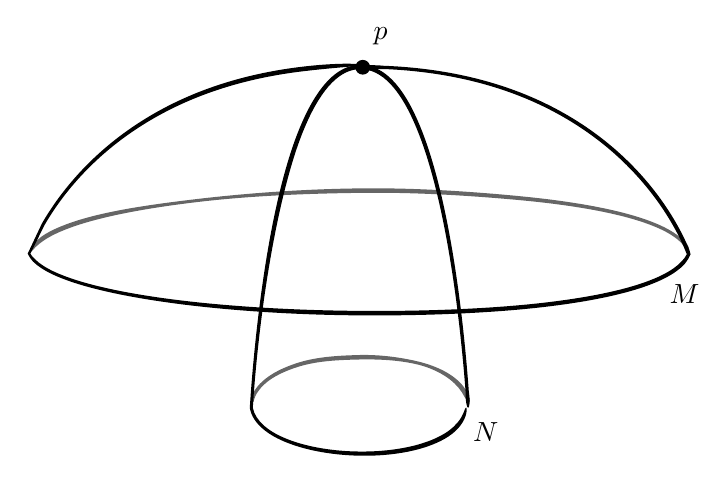
\begin{tikzpicture}[y=0.80pt, x=0.8pt,yscale=-1,scale=0.6, inner sep=0pt, outer sep=0pt]
\begin{scope}[shift={(-102.81427,-268.44763)}]% layer1
  % path5288
  \path[fill=c666666] (114.3057,422.7104) .. controls (114.4967,422.5760) and
    (114.6889,422.4426) .. (114.8823,422.3103) .. controls (114.8823,422.3103) and
    (114.8823,422.3103) .. (114.8823,422.3103) .. controls (120.2713,418.6260) and
    (126.3787,415.8955) .. (132.6430,413.4856) .. controls (132.6430,413.4856) and
    (132.6430,413.4856) .. (132.6430,413.4856) .. controls (140.8462,410.3389) and
    (149.3390,407.8786) .. (157.9265,405.7325) .. controls (168.2989,403.1415) and
    (178.8084,401.0478) .. (189.3742,399.2242) .. controls (203.5256,396.7818) and
    (217.7650,394.8161) .. (232.0518,393.1398) .. controls (243.2347,391.8276) and
    (254.4568,390.7902) .. (265.6930,389.9336) .. controls (294.3241,387.7514) and
    (323.0507,386.8117) .. (351.7812,386.4302) .. controls (351.7812,386.4302) and
    (351.7812,386.4302) .. (351.7812,386.4302) .. controls (352.8713,386.4157) and
    (353.9615,386.4021) .. (355.0516,386.3892) .. controls (382.6755,386.0628) and
    (410.3042,387.1442) .. (437.8417,389.0303) .. controls (451.2741,389.9508) and
    (464.6888,391.0445) .. (478.0719,392.3464) .. controls (490.1635,393.5227) and
    (502.2194,394.9828) .. (514.2188,396.8195) .. controls (524.8187,398.4421) and
    (535.3649,400.3632) .. (545.7809,402.8217) .. controls (554.4413,404.8671) and
    (563.0129,407.2553) .. (571.2992,410.4023) .. controls (571.2992,410.4023) and
    (571.2992,410.4023) .. (571.2992,410.4023) .. controls (577.7147,412.8438) and
    (583.9899,415.6789) .. (589.5464,419.5941) .. controls (589.5464,419.5941) and
    (589.5464,419.5941) .. (589.5464,419.5941) .. controls (591.4022,420.9016) and
    (593.1687,422.3283) .. (594.7508,423.9270) .. controls (595.0044,424.2520) and
    (595.2452,424.5639) .. (595.4747,424.8628) .. controls (596.8846,426.7020) and
    (597.8693,428.0413) .. (598.6475,428.8879) .. controls (599.4257,429.7345) and
    (600.0133,430.0872) .. (600.3869,429.8900) .. controls (600.7605,429.6928) and
    (600.9091,428.9230) .. (600.5333,427.6886) .. controls (600.1576,426.4542) and
    (599.2250,424.7552) .. (597.4902,423.0716) .. controls (597.1161,422.7079) and
    (596.7068,422.3445) .. (596.2613,421.9866) .. controls (594.6263,420.3538) and
    (592.8425,418.9042) .. (590.9925,417.5935) .. controls (590.9925,417.5935) and
    (590.9925,417.5935) .. (590.9925,417.5935) .. controls (585.1920,413.4844) and
    (578.7429,410.5213) .. (572.2319,408.0255) .. controls (572.2319,408.0255) and
    (572.2319,408.0255) .. (572.2319,408.0255) .. controls (563.8122,404.7899) and
    (555.1401,402.3307) .. (546.4169,400.2349) .. controls (535.9207,397.7118) and
    (525.3094,395.7320) .. (514.6626,394.0582) .. controls (502.8734,392.2046) and
    (491.0340,390.7135) .. (479.1653,389.4984) .. controls (465.4729,388.0967) and
    (451.7544,386.9150) .. (438.0262,385.9201) .. controls (411.0614,383.9653) and
    (384.0115,382.7961) .. (356.9728,383.0021) .. controls (355.2378,383.0153) and
    (353.4960,383.0330) .. (351.7480,383.0552) .. controls (337.7546,383.2322) and
    (323.3605,383.6956) .. (308.8819,384.4373) .. controls (294.4032,385.1790) and
    (279.8405,386.1998) .. (265.5034,387.4533) .. controls (253.8480,388.4720) and
    (242.3356,389.6349) .. (231.1414,390.9488) .. controls (216.6667,392.6476) and
    (202.7023,394.4250) .. (188.9301,396.5848) .. controls (178.2609,398.2579) and
    (167.7009,400.1692) .. (157.1753,402.6411) .. controls (148.5641,404.6623) and
    (139.9444,407.0451) .. (131.4466,410.2534) .. controls (126.2768,412.2002) and
    (121.0876,414.4491) .. (116.1906,417.3863) .. controls (115.2366,417.9721) and
    (114.1552,418.6907) .. (113.0472,419.5099) .. controls (110.9708,421.0443) and
    (108.8186,422.9904) .. (107.2686,424.9447) .. controls (106.4657,425.9554) and
    (105.8220,426.9673) .. (105.3820,427.8607) .. controls (104.9419,428.7542) and
    (104.7026,429.5261) .. (104.6355,430.0655) .. controls (104.5684,430.6048) and
    (104.6658,430.9088) .. (104.9106,430.9186) .. controls (105.1554,430.9286) and
    (105.5420,430.6437) .. (106.1759,430.0794) .. controls (107.0283,429.0527) and
    (108.0428,427.9539) .. (109.1835,426.8539) .. controls (110.7323,425.3696) and
    (112.5205,423.9371) .. (114.3057,422.7104) -- cycle;

  % path5158
  \path[fill=c666666] (434.7553,538.8076) .. controls (434.1846,537.4505) and
    (433.5108,536.1443) .. (432.7431,534.9014) .. controls (432.7431,534.9014) and
    (432.7431,534.9014) .. (432.7431,534.9014) .. controls (430.9840,532.0627) and
    (428.7928,529.5758) .. (426.3655,527.4193) .. controls (426.3655,527.4193) and
    (426.3655,527.4193) .. (426.3655,527.4193) .. controls (420.7179,522.4148) and
    (413.9759,518.9927) .. (407.0724,516.4785) .. controls (407.0724,516.4785) and
    (407.0724,516.4785) .. (407.0724,516.4785) .. controls (403.8586,515.3027) and
    (400.5876,514.3137) .. (397.2779,513.4974) .. controls (392.0666,512.2122) and
    (386.7979,511.1979) .. (381.5098,510.4005) .. controls (372.0105,508.9659) and
    (362.3885,508.2466) .. (352.7869,508.4671) .. controls (352.7869,508.4671) and
    (352.7869,508.4671) .. (352.7869,508.4671) .. controls (352.5523,508.4721) and
    (352.3178,508.4784) .. (352.0832,508.4849) .. controls (342.6896,508.7449) and
    (333.2753,509.1503) .. (323.9273,510.4535) .. controls (318.1696,511.2543) and
    (312.4212,512.3951) .. (306.8421,514.1345) .. controls (303.9351,515.0408) and
    (301.0621,516.0594) .. (298.2372,517.2071) .. controls (298.2372,517.2071) and
    (298.2372,517.2071) .. (298.2372,517.2071) .. controls (291.3983,519.9724) and
    (284.7073,523.5514) .. (279.2163,528.6151) .. controls (279.2163,528.6151) and
    (279.2163,528.6151) .. (279.2163,528.6151) .. controls (276.9203,530.7340) and
    (274.8589,533.1482) .. (273.2698,535.8618) .. controls (273.2698,535.8618) and
    (273.2698,535.8618) .. (273.2698,535.8618) .. controls (272.3224,537.4810) and
    (271.5594,539.2081) .. (271.0230,540.9977) .. controls (270.4038,541.9281) and
    (270.3001,542.7535) .. (270.4620,543.3165) .. controls (270.6239,543.8794) and
    (271.0471,544.1895) .. (271.5049,544.2492) .. controls (271.9626,544.3089) and
    (272.4541,544.1284) .. (272.8096,543.7143) .. controls (273.1651,543.3001) and
    (273.3823,542.6582) .. (273.3673,541.6712) .. controls (273.8569,540.1183) and
    (274.5441,538.6110) .. (275.3880,537.1903) .. controls (275.3880,537.1903) and
    (275.3880,537.1903) .. (275.3880,537.1903) .. controls (276.8404,534.7421) and
    (278.7671,532.5401) .. (280.9309,530.5721) .. controls (280.9309,530.5721) and
    (280.9309,530.5721) .. (280.9309,530.5721) .. controls (286.1266,525.8419) and
    (292.5789,522.5076) .. (299.2602,519.8628) .. controls (299.2602,519.8628) and
    (299.2602,519.8628) .. (299.2602,519.8628) .. controls (301.9290,518.8095) and
    (304.6451,517.8743) .. (307.3962,517.0413) .. controls (312.9455,515.3611) and
    (318.6841,514.2915) .. (324.4470,513.5521) .. controls (333.4109,512.4043) and
    (342.4303,512.0846) .. (351.4320,511.8710) .. controls (351.8965,511.8600) and
    (352.3623,511.8499) .. (352.8295,511.8407) .. controls (361.9976,511.6632) and
    (371.6772,511.8844) .. (381.1322,512.9760) .. controls (386.5370,513.6018) and
    (391.8668,514.4941) .. (396.9185,515.7585) .. controls (400.1381,516.5643) and
    (403.2268,517.5803) .. (406.1965,518.7788) .. controls (406.1965,518.7788) and
    (406.1965,518.7788) .. (406.1965,518.7788) .. controls (409.5512,520.1372) and
    (412.7700,521.7185) .. (415.7755,523.5485) .. controls (418.7810,525.3784) and
    (421.5732,527.4526) .. (424.1025,529.8537) .. controls (426.2286,531.8671) and
    (428.1573,534.0982) .. (429.7274,536.6171) .. controls (430.1291,537.2596) and
    (430.5077,537.9228) .. (430.8615,538.6057) .. controls (431.1749,539.1682) and
    (431.5945,539.8754) .. (432.0310,540.6095) .. controls (432.4676,541.3436) and
    (432.9202,542.1054) .. (433.3525,542.7411) .. controls (433.7848,543.3767) and
    (434.2005,543.8864) .. (434.5969,544.0738) .. controls (434.9934,544.2613) and
    (435.3811,544.1250) .. (435.6854,543.4331) .. controls (435.8688,542.0003) and
    (435.3243,540.2703) .. (434.7553,538.8076) -- cycle;

  % path5156
  \path[color=black,fill=black,nonzero rule,line width=0.800pt]
    (422.8475,562.9937) .. controls (418.0570,567.2954) and (412.0979,570.3812) ..
    (405.8926,572.8293) .. controls (397.9793,575.9320) and (389.5944,577.8933) ..
    (381.0980,579.1975) .. controls (381.0980,579.1975) and (381.0980,579.1975) ..
    (381.0980,579.1975) .. controls (371.7656,580.6265) and (362.2942,581.2190) ..
    (352.8223,581.1385) .. controls (352.8223,581.1385) and (352.8223,581.1385) ..
    (352.8223,581.1385) .. controls (343.3253,581.0565) and (333.8310,580.2962) ..
    (324.4640,578.7533) .. controls (324.4640,578.7533) and (324.4640,578.7533) ..
    (324.4640,578.7533) .. controls (315.9035,577.3410) and (307.4447,575.3061) ..
    (299.3828,572.2255) .. controls (299.3828,572.2255) and (299.3828,572.2255) ..
    (299.3828,572.2255) .. controls (292.6987,569.6608) and (286.2321,566.4473) ..
    (280.9374,561.8270) .. controls (278.7342,559.9063) and (276.7514,557.7490) ..
    (275.2192,555.3219) .. controls (273.8045,553.1340) and (272.7700,550.7037) ..
    (272.2889,548.1742) .. controls (272.5348,544.6751) and (272.7793,541.1738) ..
    (273.0220,537.6697) .. controls (273.0310,537.5467) and (273.0390,537.4236) ..
    (273.0476,537.3006) .. controls (273.0476,537.3006) and (273.0476,537.3006) ..
    (273.0476,537.3006) .. controls (273.7680,527.6091) and (274.6420,517.9261) ..
    (275.6375,508.2535) .. controls (275.6375,508.2535) and (275.6375,508.2534) ..
    (275.6375,508.2534) .. controls (278.6760,478.7311) and (282.7905,449.3047) ..
    (288.4156,420.1670) .. controls (291.4657,404.3690) and (294.9626,388.6596) ..
    (299.2411,373.1673) .. controls (300.4174,368.9098) and (301.6471,364.6661) ..
    (302.9537,360.4493) .. controls (305.9321,350.8370) and (309.3643,341.3804) ..
    (313.5172,332.2477) .. controls (316.0615,326.6528) and (318.8784,321.1909) ..
    (322.1430,316.0253) .. controls (324.9521,311.5842) and (328.0756,307.3560) ..
    (331.7159,303.6611) .. controls (331.7159,303.6611) and (331.7159,303.6611) ..
    (331.7159,303.6611) .. controls (334.8104,300.5263) and (338.2696,297.7646) ..
    (342.1375,295.8870) .. controls (345.6457,294.1786) and (349.5189,293.2207) ..
    (353.3666,293.2589) .. controls (357.3519,293.2873) and (361.3290,294.2969) ..
    (364.9167,296.0667) .. controls (368.8119,297.9802) and (372.2869,300.7694) ..
    (375.3875,303.9391) .. controls (375.3875,303.9391) and (375.3875,303.9391) ..
    (375.3875,303.9391) .. controls (378.9997,307.6397) and (382.0857,311.8756) ..
    (384.8592,316.3289) .. controls (384.8592,316.3289) and (384.8592,316.3289) ..
    (384.8592,316.3289) .. controls (388.0672,321.4864) and (390.8244,326.9398) ..
    (393.3206,332.5272) .. controls (397.1726,341.1496) and (400.3970,350.0522) ..
    (403.2561,359.0970) .. controls (404.7399,363.7909) and (406.1167,368.5256) ..
    (407.4213,373.2808) .. controls (411.6533,388.7174) and (415.0407,404.3942) ..
    (417.9615,420.1622) .. controls (423.3514,449.2631) and (427.1594,478.6531) ..
    (430.0446,508.1186) .. controls (430.9601,517.4692) and (431.7769,526.8280) ..
    (432.4716,536.1946) .. controls (432.4706,536.5149) and (432.4706,536.8285) ..
    (432.4721,537.1355) .. controls (432.4937,540.7590) and (432.7394,543.4522) ..
    (433.0873,545.2627) -- (433.0873,545.2627) .. controls (433.2689,546.2081) and
    (433.4781,546.9123) .. (433.6970,547.3816) -- (433.6970,547.3816) .. controls
    (433.8088,547.6214) and (433.9230,547.7997) .. (434.0373,547.9175) --
    (434.0373,547.9175) -- (434.0373,547.9175) .. controls (434.0951,547.9770) and
    (434.1528,548.0211) .. (434.2103,548.0498) .. controls (434.2392,548.0642) and
    (434.2680,548.0747) .. (434.2967,548.0813) .. controls (434.3552,548.0948) and
    (434.4132,548.0921) .. (434.4703,548.0733) .. controls (434.4984,548.0643) and
    (434.5263,548.0509) .. (434.5539,548.0338) .. controls (434.5539,548.0338) and
    (434.5539,548.0338) .. (434.5539,548.0338) .. controls (434.6090,547.9998) and
    (434.6630,547.9503) .. (434.7156,547.8855) -- (434.7156,547.8855) .. controls
    (434.7156,547.8855) and (434.7156,547.8855) .. (434.7156,547.8855) --
    (434.7156,547.8855) .. controls (434.8202,547.7565) and (434.9191,547.5666) ..
    (435.0093,547.3169) -- (435.0093,547.3169) -- (435.0093,547.3169) .. controls
    (435.1877,546.8229) and (435.3317,546.0937) .. (435.4174,545.1370) --
    (435.4174,545.1370) .. controls (435.5849,543.2678) and (435.5298,540.5257) ..
    (435.0706,536.9686) .. controls (435.0113,536.5095) and (434.9453,536.0368) ..
    (434.8722,535.5507) .. controls (434.2094,526.3225) and (433.4291,517.1031) ..
    (432.5535,507.8931) .. controls (429.7468,478.3653) and (426.0126,448.8887) ..
    (420.6876,419.6724) .. controls (417.8023,403.8410) and (414.4413,388.0765) ..
    (410.2250,372.5253) .. controls (409.0288,368.1112) and (407.7676,363.7083) ..
    (406.4143,359.3325) .. controls (403.4708,349.8149) and (400.1264,340.4151) ..
    (396.0839,331.2864) .. controls (393.5648,325.5978) and (390.7569,320.0116) ..
    (387.4688,314.6885) .. controls (387.4688,314.6885) and (387.4688,314.6885) ..
    (387.4688,314.6885) .. controls (384.6312,310.0911) and (381.4177,305.6701) ..
    (377.6121,301.7416) .. controls (374.3458,298.3650) and (370.5902,295.3591) ..
    (366.2954,293.2193) .. controls (362.3055,291.2378) and (357.8693,290.1109) ..
    (353.3667,290.0627) .. controls (348.9780,290.0266) and (344.6246,291.0862) ..
    (340.6993,292.9989) .. controls (336.4126,295.0945) and (332.6521,298.0633) ..
    (329.3777,301.3933) .. controls (329.3777,301.3933) and (329.3777,301.3933) ..
    (329.3777,301.3933) .. controls (325.5225,305.3045) and (322.2469,309.7087) ..
    (319.3507,314.2836) .. controls (315.9779,319.6047) and (313.0808,325.1921) ..
    (310.4854,330.8812) .. controls (306.6483,339.2914) and (303.4187,347.9446) ..
    (300.5992,356.7139) .. controls (298.9551,361.8273) and (297.4319,367.0217) ..
    (295.9934,372.2654) .. controls (291.7725,387.6395) and (288.3234,403.5233) ..
    (285.3618,419.5832) .. controls (279.9533,448.9087) and (276.1385,478.8616) ..
    (273.2918,508.0080) .. controls (272.3336,517.8174) and (271.4884,527.5397) ..
    (270.7725,537.1264) .. controls (270.7423,537.5813) and (270.7120,538.0359) ..
    (270.6818,538.4901) .. controls (270.4629,541.7774) and (270.2400,545.0454) ..
    (270.0136,548.2977) .. controls (270.5592,551.2518) and (271.6978,554.0505) ..
    (273.2479,556.5583) .. controls (274.9288,559.2332) and (277.0487,561.5718) ..
    (279.3724,563.6133) .. controls (284.9984,568.5524) and (291.6855,571.9496) ..
    (298.4678,574.6007) .. controls (306.7488,577.8479) and (315.3480,580.0122) ..
    (323.9979,581.5321) .. controls (333.5055,583.2049) and (343.1253,584.0869) ..
    (352.7828,584.2668) .. controls (362.3510,584.4463) and (371.9834,583.9384) ..
    (381.5871,582.5324) .. controls (390.1848,581.2767) and (398.8142,579.3088) ..
    (407.1267,576.0704) .. controls (411.4941,574.3770) and (415.8238,572.3053) ..
    (419.8150,569.6519) .. controls (421.7141,568.3699) and (423.9227,566.6400) ..
    (425.9702,564.5617) .. controls (427.1048,563.4085) and (428.1809,562.1438) ..
    (429.1213,560.8256) .. controls (430.0617,559.5074) and (430.8652,558.1363) ..
    (431.4937,556.7941) .. controls (432.2712,555.1318) and (432.7686,553.5220) ..
    (433.0418,552.1554) .. controls (433.3150,550.7888) and (433.3697,549.6670) ..
    (433.3071,548.9325) .. controls (433.2445,548.1981) and (433.0731,547.8504) ..
    (432.8304,547.9793) .. controls (432.5877,548.1083) and (432.2810,548.7162) ..
    (431.7586,549.8367) .. controls (431.1294,551.6492) and (430.2882,553.5959) ..
    (429.1724,555.4735) .. controls (427.7429,557.8894) and (425.8298,560.2039) ..
    (423.7473,562.1703) .. controls (423.4497,562.4523) and (423.1495,562.7268) ..
    (422.8475,562.9937) -- cycle;

  % path5286
  \path[fill=black] (323.4995,290.0512) .. controls (291.0640,292.6899) and
    (258.9468,299.3931) .. (228.8126,311.6673) .. controls (200.6089,323.1607) and
    (174.3465,339.6115) .. (152.2634,360.6218) .. controls (137.1469,375.0129) and
    (123.9342,391.4567) .. (113.4927,409.5396) .. controls (110.8503,415.1504) and
    (108.2095,420.7557) .. (105.5706,426.3537) .. controls (104.6522,428.3019) and
    (103.7335,430.2492) .. (102.8143,432.1956) .. controls (103.8461,434.4202) and
    (105.2631,436.3812) .. (106.8351,438.1130) .. controls (108.7404,440.0095) and
    (110.8729,441.6257) .. (113.0819,443.0627) .. controls (113.0819,443.0627) and
    (113.0819,443.0627) .. (113.0820,443.0627) .. controls (118.8717,446.8303) and
    (125.2208,449.5603) .. (131.6165,451.9131) .. controls (131.6165,451.9131) and
    (131.6165,451.9131) .. (131.6165,451.9131) .. controls (140.0110,455.0068) and
    (148.6249,457.4218) .. (157.2871,459.5245) .. controls (167.7591,462.0674) and
    (178.3361,464.1342) .. (188.9490,465.9288) .. controls (214.3042,470.2163) and
    (239.8921,472.9989) .. (265.5174,474.9890) .. controls (294.2078,477.2176) and
    (322.9809,478.3907) .. (351.7573,478.6260) .. controls (353.6649,478.6416) and
    (355.5726,478.6531) .. (357.4803,478.6604) .. controls (384.3370,478.7632) and
    (411.2021,478.2139) .. (438.0279,476.7350) .. controls (463.6783,475.3215) and
    (489.3277,473.1163) .. (514.7576,469.1580) .. controls (514.7576,469.1580) and
    (514.7576,469.1580) .. (514.7576,469.1580) .. controls (525.4167,467.4989) and
    (536.0459,465.5201) .. (546.5611,462.9773) .. controls (555.2961,460.8666) and
    (563.9875,458.3746) .. (572.4232,455.0874) .. controls (572.4232,455.0874) and
    (572.4232,455.0874) .. (572.4232,455.0874) .. controls (578.9428,452.5554) and
    (585.4116,449.5312) .. (591.2217,445.3491) .. controls (593.5095,443.7021) and
    (595.6963,441.8363) .. (597.6240,439.6729) .. controls (599.2905,437.5731) and
    (600.7477,435.2173) .. (601.7956,432.6143) .. controls (601.6090,431.8366) and
    (601.4223,431.0592) .. (601.2356,430.2820) .. controls (600.6461,428.7303) and
    (600.0144,427.2033) .. (599.3593,425.6954) .. controls (598.0398,422.6597) and
    (596.6155,419.6751) .. (595.1060,416.7383) .. controls (593.8506,414.2956) and
    (592.5373,411.8854) .. (591.1777,409.5057) .. controls (580.8397,391.4100) and
    (567.7265,374.9645) .. (552.6908,360.6019) .. controls (530.7254,339.6215) and
    (504.5464,323.2645) .. (476.4455,311.9703) .. controls (442.8486,298.4729) and
    (406.8072,292.0946) .. (370.7187,290.7271) .. controls (364.5342,290.1656) and
    (359.9745,290.1922) .. (357.0121,290.4423) .. controls (354.0496,290.6924) and
    (352.6795,291.1680) .. (352.8255,291.6291) .. controls (352.9715,292.0901) and
    (354.6311,292.5377) .. (357.7338,292.8310) .. controls (360.8366,293.1242) and
    (365.3808,293.2624) .. (371.3326,293.1983) .. controls (406.9515,294.6825) and
    (442.4444,301.0723) .. (475.4487,314.4189) .. controls (503.2362,325.6513) and
    (529.0961,341.8730) .. (550.7397,362.6305) .. controls (565.5633,376.8464) and
    (578.4767,393.0993) .. (588.6301,410.9515) .. controls (589.6822,412.8015) and
    (590.7051,414.6677) .. (591.6930,416.5512) .. controls (593.4670,419.9331) and
    (595.1265,423.3717) .. (596.6390,426.8722) .. controls (597.2750,428.3436) and
    (597.8840,429.8226) .. (598.4473,431.3147) .. controls (598.6425,431.7180) and
    (598.8376,432.1212) .. (599.0326,432.5241) .. controls (598.1568,434.4129) and
    (596.8754,436.1360) .. (595.3885,437.6861) .. controls (593.6469,439.6422) and
    (591.6182,441.3577) .. (589.4602,442.9121) .. controls (583.9593,446.8745) and
    (577.7080,449.7642) .. (571.3099,452.2504) .. controls (571.3099,452.2504) and
    (571.3099,452.2504) .. (571.3099,452.2504) .. controls (563.0430,455.4566) and
    (554.4769,457.8907) .. (545.8213,459.9681) .. controls (535.4067,462.4664) and
    (524.8575,464.4089) .. (514.2565,466.0403) .. controls (514.2565,466.0403) and
    (514.2565,466.0403) .. (514.2565,466.0403) .. controls (488.9596,469.9333) and
    (463.4142,472.0849) .. (437.8338,473.4603) .. controls (437.8337,473.4603) and
    (437.8337,473.4603) .. (437.8337,473.4603) .. controls (412.4901,474.8221) and
    (387.1079,475.3573) .. (361.7265,475.3046) .. controls (358.4257,475.2976) and
    (355.1134,475.2800) .. (351.7905,475.2514) .. controls (323.6702,475.0092) and
    (294.7954,473.9826) .. (265.7543,471.8897) .. controls (240.2491,470.0509) and
    (214.6140,467.4434) .. (189.3859,463.3320) .. controls (189.3859,463.3320) and
    (189.3859,463.3320) .. (189.3858,463.3320) .. controls (178.7693,461.6017) and
    (168.2325,459.6018) .. (157.8671,457.1374) .. controls (149.2092,455.0780) and
    (140.6709,452.7196) .. (132.4314,449.7116) .. controls (126.0771,447.3871) and
    (119.8783,444.7436) .. (114.3408,441.1415) .. controls (114.3408,441.1415) and
    (114.3408,441.1415) .. (114.3408,441.1415) .. controls (112.2175,439.7598) and
    (110.2059,438.2451) .. (108.4543,436.4986) .. controls (108.4543,436.4986) and
    (108.4543,436.4986) .. (108.4543,436.4986) .. controls (107.0105,435.2181) and
    (105.7371,433.7913) .. (104.8612,432.1869) .. controls (105.9892,429.9030) and
    (107.1147,427.6236) .. (108.2374,425.3492) .. controls (110.6734,420.4144) and
    (113.1010,415.5043) .. (115.5211,410.6212) .. controls (126.0383,392.4881) and
    (139.2095,376.4221) .. (154.0409,362.4970) .. controls (165.0832,352.1242) and
    (177.0929,342.9808) .. (189.8268,335.0164) .. controls (202.5608,327.0520) and
    (216.0212,320.2656) .. (230.0207,314.6577) .. controls (256.3996,304.0856) and
    (284.5662,297.6291) .. (314.1290,294.4096) .. controls (318.1246,293.9547) and
    (323.1890,293.4035) .. (328.3328,292.9074) .. controls (333.4766,292.4114) and
    (338.6988,291.9700) .. (342.9924,291.5843) .. controls (347.2859,291.1986) and
    (350.6508,290.8591) .. (352.0752,290.4940) .. controls (353.4997,290.1289) and
    (352.9855,289.7198) .. (349.5019,289.3268) .. controls (345.6837,289.1417) and
    (341.3331,289.1458) .. (336.8626,289.2907) .. controls (332.3921,289.4358) and
    (327.8026,289.7225) .. (323.4995,290.0512) -- cycle;

  % path821
  \path[shift={(110.0911,307.70986)},fill=black,nonzero rule] (250.5035,-15.8591)
    .. controls (250.5035,-12.7904) and (248.0159,-10.3027) .. (244.9471,-10.3027)
    .. controls (241.8784,-10.3027) and (239.3907,-12.7904) .. (239.3907,-15.8591)
    .. controls (239.3907,-18.9278) and (241.8784,-21.4155) .. (244.9471,-21.4155)
    .. controls (248.0159,-21.4155) and (250.5035,-18.9278) .. (250.5035,-15.8591)
    -- cycle;

  % text823
  \path[shift={(102.81427,289.18477)},fill=black] (260.35834,-14.107141)
    node[above right] (text823) {$p$};

  % text827
  \path[shift={(102.81427,289.18477)},fill=black] (483.17508,180.82475) node[above
    right] (text827) {$M$};

  % text831
  \path[shift={(102.81427,289.18477)},fill=black] (335.26376,284.64987) node[above
    right] (text831) {$N$};

\end{scope}

\end{tikzpicture}


\end{center}
\end{frame}
%%%%%%next-slide%%%%%
\begin{frame}[<+->]
Spróbujmy zdefiniować krzywiznę w punkcie $p\in M$ następująco:
\begin{itemize}
\item Ustalmy punkt $p\in M$ i lokalny układ współrzędnych $x\colon U\to M$ wokół $p$.
\item Wybierzmy niewielkie otoczenie otwarte $V\subset x(U)$ zawierające punkt $p$.
\item Kiedy punkt $p$ należy do zbioru $V$, wtedy $\widehat{n}(p)$ należy do zbioru $\widehat{n}(V)\subset S^2$,
\item zbadajmy więc stosunek \textbf{pól powierzchni}\[\frac{A(\widehat{n}(V)),\, \widehat{n}(V)\subset S^2 }{A(V),\, V\subset M};\]
\item Gauss definiował krzywiznę jako \[K_{\mathcal{G}}(p)\define\varinjlim_{V\to p}\frac{A(\widehat{n}(V))}{A(V)}.\]
\end{itemize}
\end{frame}
%%%%%%next-slide%%%%%
\begin{frame}[<+->]

\begin{enumerate}
\item [] Problemy:
\item Czy ta granica jest niezależna od wyboru otoczeń $V$? Jak to formalnie zdefiniować?
\item Jak zdefiniować pole wyznaczone przez $\widehat{n}(V)$ kiedy $\widehat{n}$ nie jest injekcją?
\item Co się stanie jeśli odwzorowanie Gaussa ``odwraca'' obszar $V$? Czy wtedy należałoby brać pole $A(\widehat{n}(V))$ ze znakiem ujemnym?
\end{enumerate}

\end{frame}
%%%%%%next-slide%%%%%
\begin{frame}

\begin{przyklad}
Niech $S^2\subset \R^3$ oznacza sferę o promieniu $R$ i środku w punkcie $(0,0,0)$ i niech 
\[x(\phi,\psi)=(R \cos \phi\cos \psi , R \sin \phi \cos \psi , R \sin \psi)\] będzie na niej lokalnym układem współrzędnych. \pause Mamy 
\begin{align*}
x_\phi=&R(-\sin \phi \cos \psi,\cos \phi\cos \psi,0), \\
x_\psi=&R(-\cos\phi\sin\psi,-\sin\phi\sin\psi,\cos\psi),
\end{align*}
więc jeśli wybierzemy (zgodnie z konwencją) wektor normalny $n$ wskazujący na zewnątrz, wtedy
\[\widehat{n}(p)=\frac{x_\phi\times x_\psi}{\|x_\phi\times x_\psi\|}=\frac{p}{R}\]
dla całej sfery. 
\end{przyklad}
\end{frame}
%%%%%%next-slide%%%%%
\begin{frame}
Widzimy więc, że odwzorowanie Gaussa zmiejsza obszar o czynnik $\frac{1}{R^2}$ i nie ma żadnych problemów z definicją.
\begin{center}

\definecolor{c00ff00}{RGB}{0,255,0}
\definecolor{c666666}{RGB}{102,102,102}
\definecolor{c0000ff}{RGB}{0,0,255}
\definecolor{cff0000}{RGB}{255,0,0}
\usetikzlibrary{arrows}


\mode<presentation>{\begin{tikzpicture}[y=0.80pt, x=0.8pt,yscale=-1,scale=0.4, inner sep=0pt, outer sep=0pt]}
\mode<article>{\begin{tikzpicture}[y=0.80pt, x=0.8pt,yscale=-1,scale=0.5, inner sep=0pt, outer sep=0pt]}
\begin{scope}[shift={(19.44451,-318.97965)}]% layer1
  \begin{scope}[shift={(-2093.8013,-1176.4989)}]% g2765
    % path2723
    \path[shift={(5.63871,301.66294)},draw=black,fill=c00ff00,opacity=0.300,line
      join=miter,line cap=butt,line width=0.800pt] (2247.6950,1439.1237) --
      (2158.8971,1400.6190) -- (2160.9412,1507.5149) -- cycle;

    % path2725
    \path[draw=black,line join=miter,line cap=butt,line width=0.800pt]
      (2228.2745,1730.5183) .. controls (2224.0014,1739.3592) and
      (2226.5378,1750.8854) .. (2232.2200,1757.4314);

    \begin{scope}% g1864
      \begin{scope}% g1829
        % path53-07
        \path[fill=black] (2076.2890,1785.5453) .. controls (2082.2440,1820.7310) and
          (2098.6897,1854.0943) .. (2123.6736,1879.5151) .. controls
          (2123.6736,1879.5151) and (2123.6736,1879.5151) .. (2123.6736,1879.5151) ..
          controls (2139.2415,1895.3473) and (2157.9399,1908.0777) ..
          (2178.3879,1916.7174) .. controls (2178.3879,1916.7174) and
          (2178.3879,1916.7174) .. (2178.3879,1916.7174) .. controls
          (2200.0676,1925.8742) and (2223.6309,1930.3748) .. (2247.1352,1930.2894) ..
          controls (2247.1352,1930.2894) and (2247.1352,1930.2894) ..
          (2247.1352,1930.2894) .. controls (2250.3350,1930.2784) and
          (2253.5345,1930.1717) .. (2256.7279,1929.9709) .. controls
          (2276.9017,1928.7023) and (2296.8385,1923.7387) .. (2315.1438,1915.1676) ..
          controls (2335.2206,1905.7635) and (2353.2646,1892.1457) ..
          (2368.0746,1875.6461) .. controls (2368.0746,1875.6461) and
          (2368.0746,1875.6461) .. (2368.0746,1875.6461) .. controls
          (2382.7576,1859.2884) and (2394.3083,1840.1331) .. (2402.0019,1819.5303) ..
          controls (2409.0519,1800.6541) and (2412.8523,1780.5351) ..
          (2412.9223,1760.3818) .. controls (2412.9323,1758.5032) and
          (2412.9043,1756.6243) .. (2412.8473,1754.7461) .. controls
          (2412.8473,1754.7461) and (2412.8473,1754.7461) .. (2412.8473,1754.7461) ..
          controls (2412.2130,1733.7935) and (2407.6601,1712.9780) ..
          (2399.5873,1693.6310) .. controls (2391.5145,1674.2839) and
          (2379.9182,1656.4066) .. (2365.1935,1641.3951) .. controls
          (2365.1935,1641.3951) and (2365.1935,1641.3951) .. (2365.1935,1641.3951) ..
          controls (2350.8239,1626.7529) and (2333.6372,1614.8469) ..
          (2314.7936,1606.6383) .. controls (2314.7936,1606.6383) and
          (2314.7936,1606.6383) .. (2314.7936,1606.6383) .. controls
          (2296.0792,1598.4889) and (2275.7835,1594.0409) .. (2255.3920,1593.4642) ..
          controls (2254.4294,1593.4372) and (2253.4666,1593.4182) ..
          (2252.5038,1593.4082) .. controls (2230.2186,1593.1727) and
          (2207.9916,1597.5251) .. (2187.2795,1605.5680) .. controls
          (2166.4674,1613.6468) and (2147.1165,1625.4365) .. (2130.4692,1640.2553) ..
          controls (2130.4692,1640.2553) and (2130.4691,1640.2553) ..
          (2130.4691,1640.2553) .. controls (2113.9244,1654.9799) and
          (2100.0519,1672.7729) .. (2090.4193,1692.6854) .. controls
          (2090.4193,1692.6854) and (2090.4193,1692.6854) .. (2090.4193,1692.6854) ..
          controls (2083.0433,1707.9369) and (2078.2635,1724.4271) ..
          (2076.4034,1741.2188) .. controls (2075.4383,1746.9680) and
          (2075.3522,1751.2728) .. (2075.5543,1754.0606) .. controls
          (2075.7563,1756.8483) and (2076.2457,1758.1319) .. (2076.7067,1757.9954) ..
          controls (2077.1677,1757.8589) and (2077.6034,1756.3102) ..
          (2077.9529,1753.4338) .. controls (2078.3025,1750.5575) and
          (2078.5681,1746.3562) .. (2078.9029,1740.8369) .. controls
          (2080.8145,1724.5592) and (2085.5192,1708.5822) .. (2092.7008,1693.8042) ..
          controls (2092.7008,1693.8042) and (2092.7008,1693.8042) ..
          (2092.7008,1693.8042) .. controls (2102.2081,1674.2342) and
          (2115.9119,1656.7398) .. (2132.2384,1642.2607) .. controls
          (2132.2384,1642.2607) and (2132.2384,1642.2607) .. (2132.2384,1642.2606) ..
          controls (2148.6720,1627.6891) and (2167.7701,1616.1074) ..
          (2188.2863,1608.1894) .. controls (2208.7035,1600.3116) and
          (2230.5832,1596.0680) .. (2252.4637,1596.3465) .. controls
          (2252.8727,1596.3565) and (2253.2816,1596.3585) .. (2253.6905,1596.3665) ..
          controls (2274.2579,1596.7830) and (2294.7553,1601.2118) ..
          (2313.5759,1609.4581) .. controls (2313.5759,1609.4581) and
          (2313.5760,1609.4581) .. (2313.5760,1609.4582) .. controls
          (2332.0375,1617.5453) and (2348.8726,1629.2625) .. (2362.9295,1643.6416) ..
          controls (2362.9295,1643.6416) and (2362.9295,1643.6416) ..
          (2362.9295,1643.6416) .. controls (2377.3338,1658.3688) and
          (2388.6709,1675.9248) .. (2396.5570,1694.9131) .. controls
          (2404.4432,1713.9013) and (2408.8820,1734.3206) .. (2409.4837,1754.8432) ..
          controls (2409.4837,1754.8432) and (2409.4837,1754.8432) ..
          (2409.4837,1754.8432) .. controls (2409.4997,1755.3786) and
          (2409.5127,1755.9141) .. (2409.5227,1756.4496) .. controls
          (2409.9278,1777.0886) and (2406.3533,1798.3061) .. (2398.9583,1818.3964) ..
          controls (2391.5541,1838.5065) and (2380.3307,1857.5012) ..
          (2365.9486,1873.7436) .. controls (2365.9486,1873.7437) and
          (2365.9486,1873.7437) .. (2365.9486,1873.7437) .. controls
          (2351.4372,1890.1311) and (2333.6696,1903.6776) .. (2314.1086,1912.9565) ..
          controls (2295.4530,1921.8100) and (2275.2134,1926.6895) ..
          (2255.2435,1927.7714) .. controls (2252.5350,1927.9181) and
          (2249.8309,1927.9941) .. (2247.1348,1928.0005) .. controls
          (2223.4437,1928.0555) and (2200.3516,1923.3400) .. (2179.4095,1914.3123) ..
          controls (2159.2467,1905.6231) and (2141.0712,1892.9840) ..
          (2125.9053,1877.3327) .. controls (2114.9816,1866.0651) and
          (2105.7028,1853.2031) .. (2098.2169,1839.1576) .. controls
          (2090.7311,1825.1120) and (2085.0341,1809.8777) .. (2081.4325,1793.8370) ..
          controls (2080.5922,1790.1841) and (2079.6128,1785.5371) ..
          (2078.7882,1780.7885) .. controls (2077.9636,1776.0399) and
          (2077.2965,1771.1919) .. (2076.7953,1767.1909) .. controls
          (2076.2941,1763.1899) and (2075.9403,1760.0370) .. (2075.5721,1758.7000) ..
          controls (2075.3880,1758.0315) and (2075.1992,1757.8172) ..
          (2075.0026,1758.1806) .. controls (2074.8060,1758.5439) and
          (2074.6001,1759.4851) .. (2074.4205,1761.1292) .. controls
          (2074.2722,1764.7301) and (2074.3845,1768.8344) .. (2074.7238,1773.0359) ..
          controls (2075.0639,1777.2374) and (2075.6317,1781.5344) ..
          (2076.2890,1785.5453) -- cycle;

        % path55-9
        \path[fill=black] (2279.9949,1924.5390) .. controls (2294.0493,1916.3240) and
          (2306.7867,1905.8789) .. (2316.9937,1893.2272) .. controls
          (2328.0700,1879.4775) and (2336.0250,1863.3633) .. (2340.8002,1846.4325) ..
          controls (2340.8002,1846.4325) and (2340.8002,1846.4325) ..
          (2340.8002,1846.4325) .. controls (2341.2590,1844.8059) and
          (2341.6898,1843.1724) .. (2342.0932,1841.5328) .. controls
          (2345.6816,1826.9491) and (2347.3341,1811.9301) .. (2347.4639,1796.9339) ..
          controls (2347.5958,1781.9138) and (2346.2273,1766.8785) ..
          (2343.4472,1752.1140) .. controls (2343.4471,1752.1140) and
          (2343.4471,1752.1140) .. (2343.4471,1752.1140) .. controls
          (2342.4520,1746.8338) and (2341.1782,1741.6160) .. (2339.6617,1736.4708) ..
          controls (2336.4203,1725.4727) and (2332.2702,1714.7403) ..
          (2327.5020,1704.3256) .. controls (2327.5020,1704.3256) and
          (2327.5020,1704.3256) .. (2327.5020,1704.3256) .. controls
          (2319.2447,1686.2740) and (2308.8653,1669.0495) .. (2295.8208,1653.9718) ..
          controls (2293.1301,1650.8593) and (2290.3182,1647.8396) ..
          (2287.3864,1644.9389) .. controls (2275.7497,1633.4255) and
          (2262.4175,1623.5934) .. (2247.5633,1616.7521) .. controls
          (2247.5633,1616.7521) and (2247.5633,1616.7521) .. (2247.5633,1616.7520) ..
          controls (2238.0836,1612.3912) and (2228.0261,1609.3011) ..
          (2217.7420,1607.7035) .. controls (2209.0289,1606.3516) and
          (2200.1806,1606.0768) .. (2191.4301,1606.7785) .. controls
          (2188.9705,1606.6483) and (2187.1813,1606.9262) .. (2186.0513,1607.3318) ..
          controls (2184.9213,1607.7374) and (2184.4456,1608.2716) ..
          (2184.5591,1608.7221) .. controls (2184.6726,1609.1725) and
          (2185.3716,1609.5405) .. (2186.6001,1609.6656) .. controls
          (2187.8286,1609.7908) and (2189.5836,1609.6756) .. (2191.8679,1609.1936) ..
          controls (2200.3504,1608.5721) and (2208.9090,1608.8873) ..
          (2217.3167,1610.2332) .. controls (2227.3504,1611.8372) and
          (2237.1624,1614.9041) .. (2246.4048,1619.2066) .. controls
          (2246.4048,1619.2066) and (2246.4048,1619.2066) .. (2246.4048,1619.2066) ..
          controls (2260.6949,1625.8526) and (2273.5481,1635.3845) ..
          (2284.8180,1646.5442) .. controls (2287.8582,1649.5546) and
          (2290.7691,1652.6974) .. (2293.5498,1655.9417) .. controls
          (2306.3202,1670.8478) and (2316.4589,1687.8801) .. (2324.5427,1705.7199) ..
          controls (2324.5427,1705.7199) and (2324.5427,1705.7199) ..
          (2324.5428,1705.7199) .. controls (2328.9810,1715.5270) and
          (2332.8681,1725.5804) .. (2335.9583,1735.8323) .. controls
          (2337.6132,1741.3226) and (2339.0476,1746.9632) .. (2340.1736,1752.7297) ..
          controls (2342.9772,1767.0681) and (2344.6367,1782.0184) ..
          (2344.7435,1796.9177) .. controls (2344.7965,1804.5441) and
          (2344.4441,1812.1612) .. (2343.6250,1819.6374) .. controls
          (2342.8060,1827.1135) and (2341.5198,1834.4481) .. (2339.7469,1841.5164) ..
          controls (2339.3865,1842.9530) and (2339.0039,1844.3781) ..
          (2338.5992,1845.7915) .. controls (2338.5992,1845.7915) and
          (2338.5992,1845.7915) .. (2338.5992,1845.7915) .. controls
          (2336.1472,1854.3558) and (2332.8584,1862.4816) .. (2328.8416,1870.0860) ..
          controls (2324.8249,1877.6905) and (2320.0821,1884.7773) ..
          (2314.6264,1891.2947) .. controls (2310.0347,1896.7880) and
          (2304.9440,1901.8519) .. (2299.4166,1906.5483) .. controls
          (2293.8892,1911.2447) and (2287.9241,1915.5748) .. (2281.5432,1919.5697) ..
          controls (2280.2223,1920.4199) and (2278.5591,1921.5162) ..
          (2276.8696,1922.6367) .. controls (2275.1801,1923.7571) and
          (2273.4641,1924.9015) .. (2272.0737,1925.8986) .. controls
          (2270.6834,1926.8958) and (2269.6202,1927.7492) .. (2269.2615,1928.3134) ..
          controls (2268.9029,1928.8775) and (2269.2515,1929.1603) ..
          (2270.6782,1928.9558) .. controls (2273.5981,1928.0628) and
          (2277.0193,1926.2289) .. (2279.9949,1924.5390) -- cycle;

        % path57-3
        \path[fill=black] (2186.4179,1912.8450) .. controls (2180.6417,1909.1358) and
          (2175.2555,1904.8487) .. (2170.5134,1899.9113) .. controls
          (2170.5134,1899.9113) and (2170.5134,1899.9113) .. (2170.5134,1899.9113) ..
          controls (2163.1300,1892.2432) and (2157.3732,1882.9998) ..
          (2153.2771,1873.0811) .. controls (2153.2771,1873.0811) and
          (2153.2770,1873.0811) .. (2153.2770,1873.0811) .. controls
          (2148.3529,1861.1663) and (2145.6677,1848.3561) .. (2144.0541,1835.4431) ..
          controls (2144.0541,1835.4431) and (2144.0541,1835.4431) ..
          (2144.0541,1835.4431) .. controls (2143.4037,1830.2264) and
          (2142.9266,1824.9879) .. (2142.5847,1819.7343) .. controls
          (2141.8206,1807.9927) and (2141.8697,1796.1724) .. (2142.2982,1784.3755) ..
          controls (2143.1279,1761.4262) and (2149.5511,1738.8964) ..
          (2158.7000,1717.7582) .. controls (2158.7000,1717.7582) and
          (2158.7000,1717.7582) .. (2158.7000,1717.7582) .. controls
          (2159.2389,1716.5144) and (2159.7882,1715.2748) .. (2160.3477,1714.0395) ..
          controls (2165.2378,1703.2438) and (2171.1054,1692.8771) ..
          (2177.8333,1683.1417) .. controls (2184.5612,1673.4064) and
          (2192.1472,1664.3023) .. (2200.5012,1655.9769) .. controls
          (2200.5012,1655.9769) and (2200.5012,1655.9769) .. (2200.5013,1655.9769) ..
          controls (2209.2023,1647.3053) and (2218.7467,1639.5102) ..
          (2229.0742,1632.9502) .. controls (2229.0742,1632.9502) and
          (2229.0742,1632.9502) .. (2229.0742,1632.9502) .. controls
          (2229.1712,1632.8892) and (2229.2677,1632.8275) .. (2229.3645,1632.7663) ..
          controls (2239.4619,1626.3846) and (2250.4031,1621.3089) ..
          (2261.8815,1618.0415) .. controls (2261.8815,1618.0415) and
          (2261.8815,1618.0415) .. (2261.8815,1618.0415) .. controls
          (2273.8091,1614.6433) and (2286.3172,1613.2261) .. (2298.7387,1613.8667) ..
          controls (2310.2109,1614.4555) and (2321.5888,1616.7841) ..
          (2332.5464,1620.4347) .. controls (2334.8058,1621.5317) and
          (2336.5358,1622.1033) .. (2337.7477,1622.2798) .. controls
          (2338.9597,1622.4562) and (2339.6503,1622.2378) .. (2339.7689,1621.7880) ..
          controls (2339.8875,1621.3385) and (2339.4312,1620.6574) ..
          (2338.3333,1619.9530) .. controls (2337.2355,1619.2487) and
          (2335.4926,1618.5202) .. (2333.0713,1618.0347) .. controls
          (2322.0301,1614.3220) and (2310.5368,1611.9297) .. (2298.9031,1611.2702) ..
          controls (2286.1959,1610.5532) and (2273.3867,1611.9395) ..
          (2261.1442,1615.3632) .. controls (2261.1442,1615.3632) and
          (2261.1442,1615.3632) .. (2261.1442,1615.3632) .. controls
          (2249.5956,1618.5947) and (2238.5847,1623.5947) .. (2228.4080,1629.8937) ..
          controls (2228.1082,1630.0792) and (2227.8090,1630.2658) ..
          (2227.5106,1630.4534) .. controls (2227.5105,1630.4534) and
          (2227.5105,1630.4534) .. (2227.5105,1630.4534) .. controls
          (2216.9317,1637.1024) and (2207.1617,1644.9997) .. (2198.2716,1653.7886) ..
          controls (2198.2716,1653.7886) and (2198.2716,1653.7886) ..
          (2198.2716,1653.7886) .. controls (2189.9450,1662.0206) and
          (2182.3641,1671.0048) .. (2175.6185,1680.6040) .. controls
          (2168.8730,1690.2032) and (2162.9649,1700.4175) .. (2158.0090,1711.0585) ..
          controls (2157.1878,1712.8218) and (2156.3869,1714.6047) ..
          (2155.6073,1716.4055) .. controls (2151.0835,1726.8336) and
          (2147.2202,1737.9324) .. (2144.4494,1749.3656) .. controls
          (2141.6787,1760.7987) and (2140.0074,1772.5615) .. (2139.7379,1784.2857) ..
          controls (2139.4602,1796.5397) and (2139.5662,1808.7033) ..
          (2140.3456,1820.4512) .. controls (2140.6880,1825.6127) and
          (2141.1305,1830.6963) .. (2141.7068,1835.7203) .. controls
          (2141.7068,1835.7203) and (2141.7068,1835.7203) .. (2141.7068,1835.7203) ..
          controls (2143.2284,1849.0100) and (2145.7217,1861.9546) ..
          (2150.5126,1874.2035) .. controls (2154.5135,1884.4245) and
          (2160.2567,1894.0754) .. (2168.0103,1902.2595) .. controls
          (2171.9587,1906.4180) and (2176.3813,1910.1622) .. (2181.1833,1913.4959) ..
          controls (2182.5568,1914.4255) and (2184.3520,1915.5200) ..
          (2186.2293,1916.5189) .. controls (2188.1066,1917.5179) and
          (2190.0640,1918.4213) .. (2191.7226,1919.0499) .. controls
          (2193.3813,1919.6786) and (2194.7379,1920.0372) .. (2195.4155,1919.9898) ..
          controls (2196.0930,1919.9418) and (2196.0871,1919.4970) ..
          (2195.0743,1918.4625) .. controls (2192.6173,1916.6249) and
          (2189.2637,1914.7231) .. (2186.4179,1912.8450) -- cycle;

        % path59-1
        \path[fill=black] (2405.8510,1767.6672) .. controls (2404.5404,1769.8874) and
          (2403.0260,1772.0076) .. (2401.3577,1774.0040) .. controls
          (2401.3577,1774.0040) and (2401.3577,1774.0040) .. (2401.3577,1774.0040) ..
          controls (2397.3449,1778.8048) and (2392.4441,1782.9078) ..
          (2387.1639,1786.4711) .. controls (2387.1639,1786.4711) and
          (2387.1639,1786.4711) .. (2387.1639,1786.4711) .. controls
          (2374.7809,1794.8286) and (2360.5066,1800.2529) .. (2345.9865,1804.5069) ..
          controls (2345.9865,1804.5069) and (2345.9865,1804.5069) ..
          (2345.9865,1804.5069) .. controls (2340.7897,1806.0265) and
          (2335.5440,1807.3831) .. (2330.2617,1808.6056) .. controls
          (2319.1175,1811.1847) and (2307.7731,1812.9773) .. (2296.3803,1814.2621) ..
          controls (2280.4398,1816.0583) and (2264.3917,1816.8502) ..
          (2248.3529,1816.7788) .. controls (2248.3529,1816.7788) and
          (2248.3529,1816.7788) .. (2248.3529,1816.7788) .. controls
          (2246.0663,1816.7688) and (2243.7796,1816.7428) .. (2241.4930,1816.7028) ..
          controls (2226.7669,1816.4430) and (2212.0652,1815.0948) ..
          (2197.4656,1813.1497) .. controls (2182.5250,1811.1574) and
          (2167.6900,1808.5468) .. (2153.0445,1805.2401) .. controls
          (2149.5286,1804.4462) and (2146.0269,1803.5933) .. (2142.5417,1802.6757) ..
          controls (2142.5417,1802.6757) and (2142.5417,1802.6757) ..
          (2142.5417,1802.6757) .. controls (2126.9485,1798.5513) and
          (2111.4732,1793.4357) .. (2098.2026,1784.5618) .. controls
          (2098.2026,1784.5618) and (2098.2026,1784.5618) .. (2098.2026,1784.5618) ..
          controls (2093.0096,1781.0854) and (2088.1881,1776.9993) ..
          (2084.6164,1771.9537) .. controls (2084.6164,1771.9537) and
          (2084.6164,1771.9537) .. (2084.6164,1771.9537) .. controls
          (2082.5560,1769.0475) and (2080.9559,1765.7885) .. (2079.9927,1762.3560) ..
          controls (2079.7669,1760.3458) and (2079.5064,1758.9418) ..
          (2079.1383,1758.0148) .. controls (2078.7702,1757.0879) and
          (2078.2975,1756.6457) .. (2077.8391,1756.7154) .. controls
          (2077.3807,1756.7854) and (2076.9383,1757.3824) .. (2076.7998,1758.5030) ..
          controls (2076.6612,1759.6237) and (2076.8368,1761.2806) ..
          (2077.7028,1763.2147) .. controls (2078.7257,1766.8541) and
          (2080.3961,1770.2951) .. (2082.5521,1773.3674) .. controls
          (2082.5521,1773.3674) and (2082.5521,1773.3674) .. (2082.5521,1773.3674) ..
          controls (2086.3497,1778.7672) and (2091.3680,1783.1039) ..
          (2096.7235,1786.7120) .. controls (2096.7235,1786.7120) and
          (2096.7235,1786.7120) .. (2096.7236,1786.7120) .. controls
          (2110.3508,1795.9035) and (2126.0815,1801.2438) .. (2141.7825,1805.4583) ..
          controls (2141.7825,1805.4583) and (2141.7825,1805.4583) ..
          (2141.7825,1805.4583) .. controls (2145.1113,1806.3541) and
          (2148.4543,1807.1913) .. (2151.8093,1807.9746) .. controls
          (2166.7554,1811.4641) and (2181.8813,1814.2269) .. (2197.0928,1816.3280) ..
          controls (2211.3049,1818.2929) and (2225.6293,1819.6826) ..
          (2239.9948,1820.0397) .. controls (2242.7496,1820.1087) and
          (2245.5293,1820.1450) .. (2248.3287,1820.1488) .. controls
          (2264.1577,1820.1698) and (2280.5895,1819.0114) .. (2296.6851,1816.9004) ..
          controls (2308.4873,1815.3538) and (2320.1343,1813.2992) ..
          (2331.2246,1810.7249) .. controls (2336.4692,1809.5074) and
          (2341.6005,1808.2193) .. (2346.6451,1806.8211) .. controls
          (2346.6451,1806.8211) and (2346.6451,1806.8211) .. (2346.6451,1806.8211) ..
          controls (2354.1112,1804.7548) and (2361.4342,1802.4605) ..
          (2368.5266,1799.6350) .. controls (2375.6191,1796.8096) and
          (2382.4872,1793.4544) .. (2388.9813,1789.2344) .. controls
          (2394.4408,1785.6863) and (2399.6235,1781.4593) .. (2403.9721,1776.2855) ..
          controls (2405.0399,1775.0152) and (2406.0519,1773.6849) ..
          (2406.9949,1772.2979) .. controls (2407.7568,1771.1424) and
          (2408.6242,1769.6129) .. (2409.3504,1767.9970) .. controls
          (2410.0766,1766.3810) and (2410.6577,1764.6816) .. (2410.9801,1763.2460) ..
          controls (2411.3024,1761.8105) and (2411.3741,1760.6452) ..
          (2411.1883,1760.0839) .. controls (2411.0025,1759.5226) and
          (2410.5795,1759.5717) .. (2409.7977,1760.4550) .. controls
          (2409.1700,1761.5104) and (2408.5537,1762.7298) .. (2407.9021,1763.9779) ..
          controls (2407.2504,1765.2257) and (2406.5631,1766.5026) ..
          (2405.8510,1767.6672) -- cycle;

        % path61-33
        \path[fill=black,opacity=0.280] (2409.4922,1743.2502) .. controls
          (2407.9444,1740.8908) and (2406.2065,1738.6685) .. (2404.3253,1736.5968) ..
          controls (2404.3253,1736.5968) and (2404.3253,1736.5968) ..
          (2404.3253,1736.5968) .. controls (2399.8174,1731.6318) and
          (2394.5661,1727.4726) .. (2389.0119,1723.9095) .. controls
          (2389.0119,1723.9095) and (2389.0119,1723.9095) .. (2389.0119,1723.9095) ..
          controls (2376.0166,1715.5740) and (2361.4613,1710.1384) ..
          (2346.7313,1706.0665) .. controls (2346.7313,1706.0665) and
          (2346.7313,1706.0665) .. (2346.7313,1706.0665) .. controls
          (2341.4562,1704.6053) and (2336.1362,1703.3248) .. (2330.7827,1702.2118) ..
          controls (2319.4883,1699.8635) and (2308.0822,1698.0715) ..
          (2296.6358,1696.7171) .. controls (2280.6196,1694.8206) and
          (2264.4785,1693.7852) .. (2248.3352,1693.9448) .. controls
          (2248.3352,1693.9448) and (2248.3351,1693.9448) .. (2248.3351,1693.9448) ..
          controls (2246.0350,1693.9678) and (2243.7352,1694.0128) ..
          (2241.4364,1694.0806) .. controls (2226.6310,1694.5167) and
          (2211.8367,1695.3978) .. (2197.0965,1696.8943) .. controls
          (2182.0120,1698.4238) and (2166.9323,1700.6056) .. (2152.1641,1704.1952) ..
          controls (2148.6188,1705.0569) and (2145.0882,1705.9808) ..
          (2141.5753,1706.9727) .. controls (2141.5753,1706.9727) and
          (2141.5753,1706.9727) .. (2141.5753,1706.9727) .. controls
          (2125.8911,1711.3827) and (2110.1611,1717.0221) .. (2096.7428,1726.5063) ..
          controls (2096.7428,1726.5063) and (2096.7428,1726.5063) ..
          (2096.7428,1726.5063) .. controls (2091.4695,1730.2291) and
          (2086.5713,1734.6774) .. (2082.9684,1740.1080) .. controls
          (2082.9684,1740.1080) and (2082.9684,1740.1080) .. (2082.9684,1740.1080) ..
          controls (2080.8794,1743.2608) and (2079.3138,1746.7682) ..
          (2078.4311,1750.4278) .. controls (2077.6199,1752.4015) and
          (2077.5136,1754.0064) .. (2077.6951,1755.0379) .. controls
          (2077.8765,1756.0695) and (2078.3384,1756.5446) .. (2078.8010,1756.5169) ..
          controls (2079.2636,1756.4889) and (2079.7289,1755.9743) ..
          (2080.0831,1755.0302) .. controls (2080.4374,1754.0861) and
          (2080.6799,1752.7188) .. (2080.8442,1750.8205) .. controls
          (2081.6832,1747.5375) and (2083.1302,1744.3757) .. (2085.0327,1741.5217) ..
          controls (2085.0327,1741.5217) and (2085.0327,1741.5217) ..
          (2085.0327,1741.5217) .. controls (2088.4096,1736.4454) and
          (2093.1111,1732.2477) .. (2098.2218,1728.6565) .. controls
          (2098.2218,1728.6565) and (2098.2218,1728.6565) .. (2098.2218,1728.6565) ..
          controls (2111.2836,1719.4898) and (2126.7587,1714.0750) ..
          (2142.3345,1709.7553) .. controls (2142.3345,1709.7553) and
          (2142.3345,1709.7553) .. (2142.3345,1709.7553) .. controls
          (2145.6329,1708.8428) and (2148.9479,1707.9907) .. (2152.2769,1707.1939) ..
          controls (2167.1074,1703.6446) and (2182.2759,1701.5378) ..
          (2197.4693,1700.0725) .. controls (2211.6647,1698.7054) and
          (2225.8918,1697.8995) .. (2240.1114,1697.4887) .. controls
          (2242.8382,1697.4097) and (2245.5890,1697.3507) .. (2248.3593,1697.3145) ..
          controls (2264.0088,1697.1092) and (2280.2980,1697.7536) ..
          (2296.3310,1699.3551) .. controls (2308.0878,1700.5309) and
          (2319.7072,1702.2108) .. (2330.7656,1704.5393) .. controls
          (2335.9951,1705.6404) and (2341.0899,1706.9243) .. (2346.0727,1708.3803) ..
          controls (2346.0727,1708.3803) and (2346.0727,1708.3803) ..
          (2346.0727,1708.3803) .. controls (2353.4507,1710.5394) and
          (2360.6147,1713.0492) .. (2367.4894,1716.0443) .. controls
          (2374.3640,1719.0395) and (2380.9502,1722.5137) .. (2387.1944,1726.6725) ..
          controls (2392.4320,1730.1605) and (2397.4028,1734.1302) ..
          (2401.7108,1738.8779) .. controls (2402.7657,1740.0405) and
          (2403.7802,1741.2524) .. (2404.7440,1742.5134) .. controls
          (2405.5550,1743.5421) and (2406.5781,1744.8512) .. (2407.5807,1746.2188) ..
          controls (2408.5833,1747.5865) and (2409.5626,1749.0142) ..
          (2410.3941,1750.2021) .. controls (2411.2257,1751.3900) and
          (2411.9179,1752.3359) .. (2412.4211,1752.6690) .. controls
          (2412.9243,1753.0022) and (2413.2602,1752.7140) .. (2413.2240,1751.4377) ..
          controls (2412.9548,1750.1250) and (2412.4330,1748.6963) ..
          (2411.7675,1747.2926) .. controls (2411.1020,1745.8888) and
          (2410.2938,1744.5110) .. (2409.4922,1743.2502) -- cycle;

        \begin{scope}% g1751
          \begin{scope}[cm={{0.5939,0.0,0.0,0.5939,(746.01496,1124.7564)}}]% g1650
            % path5288
            \path[fill=c666666] (2293.1459,920.1168) .. controls (2293.3836,919.9471) and
              (2293.6234,919.7792) .. (2293.8650,919.6129) .. controls (2293.8650,919.6129)
              and (2293.8650,919.6129) .. (2293.8650,919.6129) .. controls
              (2299.1053,916.0101) and (2305.0616,913.3518) .. (2311.1764,911.0213) ..
              controls (2311.1764,911.0213) and (2311.1764,911.0213) .. (2311.1764,911.0213)
              .. controls (2319.1512,907.9911) and (2327.4142,905.6492) ..
              (2335.7704,903.6246) .. controls (2345.8487,901.1842) and (2356.0612,899.2442)
              .. (2366.3276,897.5765) .. controls (2380.1011,895.3393) and
              (2393.9587,893.5844) .. (2407.8608,892.1226) .. controls (2418.6870,890.9842)
              and (2429.5492,890.1197) .. (2440.4228,889.4358) .. controls
              (2468.2172,887.6883) and (2496.0902,887.1889) .. (2523.9580,887.2528) ..
              controls (2523.9580,887.2528) and (2523.9580,887.2528) .. (2523.9580,887.2528)
              .. controls (2525.2031,887.2558) and (2526.4483,887.2598) ..
              (2527.6934,887.2647) .. controls (2554.3281,887.3734) and (2580.9452,888.8698)
              .. (2607.4577,891.1608) .. controls (2620.7787,892.3124) and
              (2634.0776,893.6463) .. (2647.3394,895.1963) .. controls (2658.8088,896.5368)
              and (2670.2390,898.1472) .. (2681.6091,900.1114) .. controls
              (2691.9205,901.8929) and (2702.1730,903.9699) .. (2712.2867,906.5724) ..
              controls (2720.7279,908.7457) and (2729.0736,911.2579) .. (2737.1257,914.5049)
              .. controls (2737.1257,914.5049) and (2737.1257,914.5049) ..
              (2737.1257,914.5049) .. controls (2743.4016,917.0406) and (2749.5277,919.9664)
              .. (2754.9414,923.9216) .. controls (2754.9414,923.9216) and
              (2754.9414,923.9216) .. (2754.9414,923.9216) .. controls (2756.8175,925.2921)
              and (2758.5989,926.7847) .. (2760.1875,928.4518) .. controls
              (2760.3904,928.7240) and (2760.5849,928.9866) .. (2760.7718,929.2397) ..
              controls (2762.1490,931.1077) and (2763.1206,932.4561) .. (2763.8957,933.3054)
              .. controls (2764.6708,934.1546) and (2765.2638,934.5032) ..
              (2765.6423,934.3035) .. controls (2766.0207,934.1037) and (2766.1738,933.3333)
              .. (2765.8038,932.1011) .. controls (2765.4339,930.8689) and
              (2764.5101,929.1750) .. (2762.7870,927.4899) .. controls (2762.4657,927.1752)
              and (2762.1181,926.8606) .. (2761.7435,926.5494) .. controls
              (2760.0993,924.8427) and (2758.2973,923.3229) .. (2756.4232,921.9454) ..
              controls (2756.4232,921.9454) and (2756.4232,921.9454) .. (2756.4232,921.9454)
              .. controls (2750.7747,917.7951) and (2744.4795,914.7389) ..
              (2738.1081,912.1455) .. controls (2738.1081,912.1455) and (2738.1081,912.1455)
              .. (2738.1081,912.1455) .. controls (2729.9250,908.8070) and
              (2721.4798,906.2215) .. (2712.9759,903.9958) .. controls (2702.7824,901.3268)
              and (2692.4652,899.1896) .. (2682.1069,897.3557) .. controls
              (2670.9414,895.3789) and (2659.7223,893.7423) .. (2648.4703,892.3680) ..
              controls (2634.9048,890.7113) and (2621.3076,889.2827) .. (2607.6965,888.0510)
              .. controls (2581.7403,885.7014) and (2555.6859,884.1276) ..
              (2529.6203,883.9085) .. controls (2527.7473,883.8927) and (2525.8659,883.8824)
              .. (2523.9772,883.8774) .. controls (2496.8110,883.8053) and
              (2468.1007,884.8873) .. (2440.2664,886.9557) .. controls (2428.9840,887.7939)
              and (2417.8383,888.7781) .. (2406.9974,889.9185) .. controls
              (2392.9100,891.4003) and (2379.3177,892.9723) .. (2365.9101,894.9338) ..
              controls (2355.5406,896.4508) and (2345.2750,898.2097) .. (2335.0426,900.5303)
              .. controls (2326.6576,902.4309) and (2318.2632,904.6958) ..
              (2309.9916,907.7860) .. controls (2304.8733,909.6931) and (2299.7369,911.9151)
              .. (2294.9052,914.8443) .. controls (2294.0259,915.3903) and
              (2293.0359,916.0542) .. (2292.0195,916.8092) .. controls (2289.9913,918.3150)
              and (2287.8764,920.2420) .. (2286.3534,922.1836) .. controls
              (2285.5654,923.1867) and (2284.9339,924.1920) .. (2284.5015,925.0810) ..
              controls (2284.0692,925.9700) and (2283.8332,926.7398) .. (2283.7672,927.2801)
              .. controls (2283.7012,927.8205) and (2283.7982,928.1291) ..
              (2284.0410,928.1460) .. controls (2284.2842,928.1629) and (2284.6685,927.8881)
              .. (2285.2948,927.3337) .. controls (2286.1466,926.3067) and
              (2287.1545,925.2013) .. (2288.2886,924.0979) .. controls (2289.7612,922.6731)
              and (2291.4528,921.2966) .. (2293.1459,920.1168) -- cycle;

            % path5286
            \path[cm={{1.68379,0.0,0.0,1.68379,(-1246.6356,-1385.9138)}},fill=black]
              (2238.5625,1292.4375) .. controls (2237.3083,1292.4475) and
              (2236.0069,1292.4725) .. (2234.6875,1292.5315) .. controls
              (2232.0484,1292.6485) and (2229.3481,1292.8490) .. (2226.8125,1293.0941) ..
              controls (2209.2000,1294.8845) and (2191.8284,1299.1669) ..
              (2175.5312,1306.0628) .. controls (2158.2700,1313.3696) and
              (2142.2397,1323.5276) .. (2128.0938,1335.8128) .. controls
              (2117.8857,1344.6772) and (2108.6168,1354.6062) .. (2100.5625,1365.4691) ..
              controls (2098.7161,1367.9591) and (2096.9448,1370.5250) ..
              (2095.2500,1373.1253) .. controls (2094.7838,1373.8405) and
              (2094.3274,1374.5572) .. (2093.8750,1375.2815) .. controls
              (2093.3088,1376.1879) and (2092.7559,1377.1029) .. (2092.2188,1378.0315) ..
              controls (2092.0792,1378.2728) and (2091.9180,1378.5050) ..
              (2091.7812,1378.7503) .. controls (2091.7452,1378.8933) and
              (2091.7242,1379.0441) .. (2091.6872,1379.1878) .. controls
              (2091.6772,1379.2238) and (2091.6652,1379.2448) .. (2091.6562,1379.2818) ..
              controls (2091.6562,1379.2928) and (2091.6562,1379.3018) ..
              (2091.6562,1379.3128) -- (2091.6562,1379.3438) .. controls
              (2092.2649,1380.6669) and (2093.0736,1381.8080) .. (2094.0000,1382.8438) ..
              controls (2095.1251,1383.9731) and (2096.4135,1384.9516) ..
              (2097.7188,1385.8125) .. controls (2101.1334,1388.0655) and
              (2104.8783,1389.7016) .. (2108.6562,1391.1250) .. controls
              (2113.6063,1392.9933) and (2118.6684,1394.4650) .. (2123.7812,1395.7500) ..
              controls (2129.9560,1397.3024) and (2136.2071,1398.5769) ..
              (2142.4688,1399.6875) .. controls (2157.4148,1402.3385) and
              (2172.5084,1404.1164) .. (2187.6250,1405.4062) .. controls
              (2204.5377,1406.8497) and (2221.4965,1407.6486) .. (2238.4688,1407.9062) ..
              controls (2238.5278,1407.9062) and (2238.5973,1407.9057) ..
              (2238.6562,1407.9062) .. controls (2255.5535,1408.1591) and
              (2272.4571,1408.0002) .. (2289.3438,1407.1875) .. controls
              (2304.4667,1406.4600) and (2319.5925,1405.2490) .. (2334.5938,1403.0000) ..
              controls (2340.8807,1402.0575) and (2347.1398,1400.9391) ..
              (2353.3438,1399.4688) .. controls (2358.4978,1398.2481) and
              (2363.6465,1396.7981) .. (2368.6250,1394.8750) .. controls
              (2372.4758,1393.3926) and (2376.2889,1391.5911) .. (2379.7188,1389.1250) ..
              controls (2381.0721,1388.1518) and (2382.3611,1387.0611) ..
              (2383.5000,1385.7812) .. controls (2384.4834,1384.5250) and
              (2385.3529,1383.1148) .. (2385.9688,1381.5625) .. controls
              (2385.8265,1381.0764) and (2385.6736,1380.5793) .. (2385.5312,1380.0938) ..
              controls (2385.1055,1379.1355) and (2384.6461,1378.2159) ..
              (2384.1875,1377.2812) .. controls (2383.8206,1376.5337) and
              (2383.4456,1375.7699) .. (2383.0625,1375.0312) .. controls
              (2381.6844,1372.3738) and (2380.2037,1369.7724) .. (2378.6562,1367.2188) ..
              controls (2371.9540,1356.1574) and (2363.8902,1345.9393) ..
              (2354.7188,1336.8438) .. controls (2342.0358,1324.2646) and
              (2327.1439,1313.9025) .. (2310.8750,1306.5938) .. controls
              (2293.1796,1298.6484) and (2274.0047,1294.4317) .. (2254.6875,1293.4062) ..
              controls (2251.0419,1293.0184) and (2248.3439,1293.0142) ..
              (2246.5938,1293.1562) .. controls (2244.8435,1293.2983) and
              (2244.0391,1293.6012) .. (2244.1250,1293.8750) .. controls
              (2244.2110,1294.1488) and (2245.1727,1294.4120) .. (2247.0000,1294.5938) ..
              controls (2248.8273,1294.7755) and (2251.4939,1294.8592) ..
              (2255.0000,1294.8750) .. controls (2274.0132,1295.9662) and
              (2292.8955,1300.1934) .. (2310.2500,1308.0312) .. controls
              (2326.3283,1315.2888) and (2341.0393,1325.5655) .. (2353.5625,1338.0312) ..
              controls (2362.6221,1347.0498) and (2370.5800,1357.1748) ..
              (2377.1875,1368.1250) .. controls (2378.5374,1370.3623) and
              (2379.8451,1372.6286) .. (2381.0625,1374.9375) .. controls
              (2381.6034,1375.9633) and (2382.1165,1376.9896) .. (2382.6250,1378.0312) ..
              controls (2383.0731,1378.9490) and (2383.4950,1379.8818) ..
              (2383.9062,1380.8125) .. controls (2384.0475,1381.0621) and
              (2384.2026,1381.3130) .. (2384.3438,1381.5625) .. controls
              (2383.8230,1382.6774) and (2383.0703,1383.6794) .. (2382.1875,1384.5938) ..
              controls (2381.1590,1385.7506) and (2379.9633,1386.7696) ..
              (2378.6875,1387.6875) .. controls (2375.4423,1390.0228) and
              (2371.7465,1391.7323) .. (2367.9688,1393.1875) .. controls
              (2363.0915,1395.0625) and (2358.0440,1396.4553) .. (2352.9375,1397.6562) ..
              controls (2346.7940,1399.1003) and (2340.5645,1400.2301) ..
              (2334.3125,1401.1562) .. controls (2319.3911,1403.3665) and
              (2304.3311,1404.5452) .. (2289.2500,1405.2500) .. controls
              (2273.2435,1405.9974) and (2257.2106,1406.1496) .. (2241.1875,1405.9375) ..
              controls (2240.2973,1405.9255) and (2239.3930,1405.9205) ..
              (2238.5000,1405.9065) .. controls (2221.9364,1405.6379) and
              (2204.9205,1404.9009) .. (2187.7812,1403.5315) .. controls
              (2172.7506,1402.3302) and (2157.6356,1400.6717) .. (2142.7500,1398.1253) ..
              controls (2136.4889,1397.0542) and (2130.2707,1395.8483) ..
              (2124.1562,1394.3441) .. controls (2119.0477,1393.0867) and
              (2114.0170,1391.6283) .. (2109.1562,1389.8128) .. controls
              (2105.4038,1388.4084) and (2101.7369,1386.8410) .. (2098.4688,1384.6878) ..
              controls (2097.2137,1383.8607) and (2096.0043,1382.9468) ..
              (2094.9688,1381.9065) .. controls (2094.1233,1381.1600) and
              (2093.3969,1380.3061) .. (2092.8750,1379.3753) .. controls
              (2092.9070,1379.3913) and (2092.9370,1379.3913) .. (2092.9690,1379.4063) ..
              controls (2093.1010,1379.1690) and (2093.2384,1378.9557) ..
              (2093.3752,1378.7189) .. controls (2093.9028,1377.8051) and
              (2094.4413,1376.8953) .. (2095.0002,1376.0001) .. controls
              (2095.5986,1375.0414) and (2096.2228,1374.0958) .. (2096.8440,1373.1563) ..
              controls (2098.3902,1370.8177) and (2099.9969,1368.5429) ..
              (2101.6564,1366.3126) .. controls (2109.8163,1355.3471) and
              (2119.0822,1345.5726) .. (2129.1252,1336.9689) .. controls
              (2136.2114,1330.8987) and (2143.7219,1325.4307) .. (2151.5940,1320.5626) ..
              controls (2159.4660,1315.6945) and (2167.6890,1311.4224) ..
              (2176.2814,1307.8439) .. controls (2190.4229,1301.9519) and
              (2205.5203,1297.9446) .. (2221.3440,1295.8126) .. controls
              (2223.6907,1295.4846) and (2226.6624,1295.0956) .. (2229.6877,1294.7501) ..
              controls (2232.7130,1294.4046) and (2235.7824,1294.0913) ..
              (2238.3127,1293.8439) .. controls (2240.8429,1293.5964) and
              (2242.8153,1293.4050) .. (2243.6564,1293.1876) .. controls
              (2244.4976,1292.9702) and (2244.2159,1292.7278) .. (2242.1564,1292.5001) ..
              controls (2241.0287,1292.4481) and (2239.8167,1292.4309) ..
              (2238.5625,1292.4375) -- cycle;

          \end{scope}
          % path1644
          \path[shift={(5.63871,301.66294)},draw=black,line join=miter,line cap=butt,line
            width=0.800pt,-latex'] (2245.9246,1317.0891) -- (2245.9246,1235.8959);

          % path1646
          \path[shift={(5.63871,301.66294)},draw=black,line join=miter,line cap=butt,line
            width=0.800pt,-latex'] (2186.8971,1358.6190) -- (2138.7051,1310.4270);

          % path1648
          \path[shift={(5.63871,301.66294)},draw=black,line join=miter,line cap=butt,line
            width=0.800pt,-latex'] (2290.1821,1352.3088) -- (2337.0650,1304.9986);

          % path5286-9
          \path[fill=c0000ff,opacity=0.300] (2243.9398,1594.8895) .. controls
            (2242.6856,1594.8995) and (2241.3842,1594.9245) .. (2240.0648,1594.9835) ..
            controls (2237.4257,1595.1005) and (2234.7254,1595.3010) ..
            (2232.1898,1595.5461) .. controls (2214.5773,1597.3365) and
            (2197.2057,1601.6189) .. (2180.9085,1608.5148) .. controls
            (2163.6473,1615.8216) and (2147.6170,1625.9796) .. (2133.4710,1638.2648) ..
            controls (2123.2630,1647.1292) and (2113.9941,1657.0582) ..
            (2105.9398,1667.9211) .. controls (2104.0934,1670.4111) and
            (2102.3221,1672.9770) .. (2100.6273,1675.5773) .. controls
            (2100.1611,1676.2925) and (2099.7047,1677.0092) .. (2099.2523,1677.7335) ..
            controls (2098.6861,1678.6399) and (2098.1332,1679.5549) ..
            (2097.5961,1680.4835) .. controls (2097.4564,1680.7248) and
            (2097.2953,1680.9570) .. (2097.1585,1681.2023) .. controls
            (2097.1225,1681.3453) and (2097.1005,1681.4961) .. (2097.0645,1681.6398) ..
            controls (2097.0545,1681.6758) and (2097.0415,1681.6968) ..
            (2097.0325,1681.7338) -- (2097.0325,1681.7648) -- (2097.0325,1681.7958) ..
            controls (2097.6412,1683.1189) and (2098.4499,1684.2600) ..
            (2099.3763,1685.2958) .. controls (2100.5014,1686.4251) and
            (2101.7898,1687.4036) .. (2103.0951,1688.2645) .. controls
            (2106.5097,1690.5175) and (2110.2546,1692.1536) .. (2114.0325,1693.5770) ..
            controls (2118.9826,1695.4453) and (2124.0447,1696.9170) ..
            (2129.1575,1698.2020) .. controls (2135.3323,1699.7544) and
            (2141.5834,1701.0289) .. (2147.8451,1702.1395) .. controls
            (2162.7911,1704.7905) and (2177.8847,1706.5684) .. (2193.0013,1707.8582) ..
            controls (2209.9140,1709.3017) and (2226.8728,1710.1006) ..
            (2243.8451,1710.3582) .. controls (2243.9041,1710.3582) and
            (2243.9736,1710.3577) .. (2244.0325,1710.3582) .. controls
            (2260.9298,1710.6111) and (2277.8334,1710.4522) .. (2294.7201,1709.6395) ..
            controls (2309.8430,1708.9120) and (2324.9688,1707.7010) ..
            (2339.9701,1705.4520) .. controls (2346.2570,1704.5095) and
            (2352.5161,1703.3911) .. (2358.7201,1701.9208) .. controls
            (2363.8741,1700.7001) and (2369.0228,1699.2501) .. (2374.0013,1697.3270) ..
            controls (2377.8521,1695.8446) and (2381.6652,1694.0431) ..
            (2385.0951,1691.5770) .. controls (2386.4484,1690.6038) and
            (2387.7374,1689.5131) .. (2388.8763,1688.2332) .. controls
            (2389.8597,1686.9770) and (2390.7292,1685.5668) .. (2391.3451,1684.0145) ..
            controls (2391.2028,1683.5284) and (2391.0499,1683.0313) ..
            (2390.9075,1682.5458) .. controls (2390.4818,1681.5875) and
            (2390.0224,1680.6679) .. (2389.5638,1679.7332) .. controls
            (2389.1969,1678.9857) and (2388.8219,1678.2219) .. (2388.4388,1677.4832) ..
            controls (2387.0607,1674.8258) and (2385.5800,1672.2244) ..
            (2384.0325,1669.6708) .. controls (2377.3303,1658.6094) and
            (2369.2665,1648.3913) .. (2360.0951,1639.2958) .. controls
            (2347.4121,1626.7166) and (2332.5202,1616.3545) .. (2316.2513,1609.0458) ..
            controls (2298.5559,1601.1004) and (2279.3717,1596.2469) ..
            (2260.0638,1595.0586) .. controls (2256.4045,1594.8334) and
            (2254.6679,1595.0346) .. (2251.9701,1595.0086) .. controls
            (2250.4908,1594.9946) and (2249.0117,1594.9746) .. (2247.5325,1594.9516) ..
            controls (2246.3354,1594.9339) and (2245.1940,1594.8829) ..
            (2243.9398,1594.8895) -- cycle;

          % path1727
          \path[draw=black,line join=miter,line cap=butt,line width=0.800pt,-latex']
            (2164.5358,1702.2819) -- (2096.3438,1656.0899);

          % path1729
          \path[draw=black,line join=miter,line cap=butt,line width=0.800pt,-latex']
            (2326.3438,1706.2819) -- (2394.5358,1660.0899);

        \end{scope}
      \end{scope}
      \begin{scope}% g1812
        % path1640
        \path[fill=black,opacity=0.280] (2847.0632,1726.8499) .. controls
          (2844.6428,1722.9358) and (2841.4206,1719.6345) .. (2837.7896,1717.0198) ..
          controls (2832.4217,1713.1516) and (2826.3439,1710.5456) ..
          (2820.1514,1708.7202) .. controls (2820.1514,1708.7202) and
          (2820.1514,1708.7202) .. (2820.1514,1708.7202) .. controls
          (2818.0593,1708.1018) and (2815.9501,1707.5621) .. (2813.8268,1707.1009) ..
          controls (2807.7517,1705.7813) and (2801.6221,1704.8094) ..
          (2795.4384,1704.1902) .. controls (2789.2548,1703.5711) and
          (2783.0225,1703.3074) .. (2776.8322,1703.4173) .. controls
          (2776.3532,1703.4273) and (2775.8742,1703.4363) .. (2775.3953,1703.4503) ..
          controls (2768.2698,1703.6537) and (2761.1341,1703.8618) ..
          (2754.0136,1704.5844) .. controls (2748.2670,1705.1651) and
          (2742.4976,1706.0814) .. (2736.9186,1707.7539) .. controls
          (2735.1483,1708.2846) and (2733.3919,1708.8656) .. (2731.6537,1709.5032) ..
          controls (2731.6537,1709.5032) and (2731.6537,1709.5032) ..
          (2731.6537,1709.5032) .. controls (2725.4952,1711.7414) and
          (2719.3820,1714.7710) .. (2714.5356,1719.3862) .. controls
          (2714.5356,1719.3862) and (2714.5356,1719.3862) .. (2714.5356,1719.3862) ..
          controls (2712.4730,1721.3540) and (2710.6870,1723.6567) ..
          (2709.4477,1726.2485) .. controls (2709.4477,1726.2485) and
          (2709.4477,1726.2485) .. (2709.4477,1726.2485) .. controls
          (2708.6193,1727.9896) and (2708.0658,1729.8436) .. (2707.7968,1731.7272) ..
          controls (2707.3455,1732.5810) and (2707.3708,1733.2951) ..
          (2707.6159,1733.7537) .. controls (2707.8610,1734.2123) and
          (2708.3234,1734.4260) .. (2708.7848,1734.4258) .. controls
          (2709.2463,1734.4256) and (2709.7077,1734.2208) .. (2709.9957,1733.8381) ..
          controls (2710.2838,1733.4554) and (2710.3962,1732.9017) ..
          (2710.2108,1732.0765) .. controls (2710.4638,1730.4656) and
          (2710.9561,1728.8838) .. (2711.6754,1727.4090) .. controls
          (2711.6754,1727.4090) and (2711.6754,1727.4090) .. (2711.6754,1727.4090) ..
          controls (2712.7677,1725.1507) and (2714.3958,1723.1136) ..
          (2716.2889,1721.3330) .. controls (2716.2889,1721.3330) and
          (2716.2889,1721.3330) .. (2716.2889,1721.3330) .. controls
          (2720.7707,1717.1085) and (2726.5993,1714.3518) .. (2732.5884,1712.2213) ..
          controls (2732.5884,1712.2213) and (2732.5884,1712.2213) ..
          (2732.5884,1712.2213) .. controls (2734.2004,1711.6511) and
          (2735.8305,1711.1310) .. (2737.4753,1710.6555) .. controls
          (2742.9844,1709.0628) and (2748.7129,1708.2377) .. (2754.4453,1707.7280) ..
          controls (2761.2442,1707.1261) and (2768.0513,1706.9897) ..
          (2774.8479,1706.8337) .. controls (2775.5142,1706.8187) and
          (2776.1838,1706.8047) .. (2776.8565,1706.7927) .. controls
          (2782.8622,1706.6947) and (2789.1205,1706.6656) .. (2795.3310,1707.0087) ..
          controls (2801.5415,1707.3518) and (2807.7045,1708.0776) ..
          (2813.4857,1709.3573) .. controls (2815.5231,1709.8083) and
          (2817.5038,1710.3607) .. (2819.4344,1710.9986) .. controls
          (2819.4344,1710.9986) and (2819.4344,1710.9986) .. (2819.4344,1710.9986) ..
          controls (2822.4663,1712.0025) and (2825.3715,1713.2233) ..
          (2828.1097,1714.6570) .. controls (2830.8479,1716.0906) and
          (2833.4186,1717.7333) .. (2835.8139,1719.6237) .. controls
          (2838.6131,1721.8359) and (2841.1673,1724.4143) .. (2843.3199,1727.4137) ..
          controls (2843.9900,1728.2804) and (2845.1007,1729.5777) ..
          (2846.0855,1730.4788) .. controls (2846.5779,1730.9294) and
          (2847.0499,1731.2727) .. (2847.4616,1731.3488) .. controls
          (2847.8733,1731.4248) and (2848.2314,1731.2308) .. (2848.4379,1730.5870) ..
          controls (2848.4307,1729.3456) and (2847.7208,1727.9937) ..
          (2847.0632,1726.8499) -- cycle;

        \begin{scope}[cm={{0.24383,0.0,0.0,0.24383,(2162.0441,1469.7571)}}]% g1697
          % path1699
          \path[fill=c666666] (2293.1459,920.1168) .. controls (2293.3836,919.9471) and
            (2293.6234,919.7792) .. (2293.8650,919.6129) .. controls (2293.8650,919.6129)
            and (2293.8650,919.6129) .. (2293.8650,919.6129) .. controls
            (2299.1053,916.0101) and (2305.0616,913.3518) .. (2311.1764,911.0213) ..
            controls (2311.1764,911.0213) and (2311.1764,911.0213) .. (2311.1764,911.0213)
            .. controls (2319.1512,907.9911) and (2327.4142,905.6492) ..
            (2335.7704,903.6246) .. controls (2345.8487,901.1842) and (2356.0612,899.2442)
            .. (2366.3276,897.5765) .. controls (2380.1011,895.3393) and
            (2393.9587,893.5844) .. (2407.8608,892.1226) .. controls (2418.6870,890.9842)
            and (2429.5492,890.1197) .. (2440.4228,889.4358) .. controls
            (2468.2172,887.6883) and (2496.0902,887.1889) .. (2523.9580,887.2528) ..
            controls (2523.9580,887.2528) and (2523.9580,887.2528) .. (2523.9580,887.2528)
            .. controls (2525.2031,887.2558) and (2526.4483,887.2598) ..
            (2527.6934,887.2647) .. controls (2554.3281,887.3734) and (2580.9452,888.8698)
            .. (2607.4577,891.1608) .. controls (2620.7787,892.3124) and
            (2634.0776,893.6463) .. (2647.3394,895.1963) .. controls (2658.8088,896.5368)
            and (2670.2390,898.1472) .. (2681.6091,900.1114) .. controls
            (2691.9205,901.8929) and (2702.1730,903.9699) .. (2712.2867,906.5724) ..
            controls (2720.7279,908.7457) and (2729.0736,911.2579) .. (2737.1257,914.5049)
            .. controls (2737.1257,914.5049) and (2737.1257,914.5049) ..
            (2737.1257,914.5049) .. controls (2743.4016,917.0406) and (2749.5277,919.9664)
            .. (2754.9414,923.9216) .. controls (2754.9414,923.9216) and
            (2754.9414,923.9216) .. (2754.9414,923.9216) .. controls (2756.8175,925.2921)
            and (2758.5989,926.7847) .. (2760.1875,928.4518) .. controls
            (2760.3904,928.7240) and (2760.5849,928.9866) .. (2760.7718,929.2397) ..
            controls (2762.1490,931.1077) and (2763.1206,932.4561) .. (2763.8957,933.3054)
            .. controls (2764.6708,934.1546) and (2765.2638,934.5032) ..
            (2765.6423,934.3035) .. controls (2766.0207,934.1037) and (2766.1738,933.3333)
            .. (2765.8038,932.1011) .. controls (2765.4339,930.8689) and
            (2764.5101,929.1750) .. (2762.7870,927.4899) .. controls (2762.4657,927.1752)
            and (2762.1181,926.8606) .. (2761.7435,926.5494) .. controls
            (2760.0993,924.8427) and (2758.2973,923.3229) .. (2756.4232,921.9454) ..
            controls (2756.4232,921.9454) and (2756.4232,921.9454) .. (2756.4232,921.9454)
            .. controls (2750.7747,917.7951) and (2744.4795,914.7389) ..
            (2738.1081,912.1455) .. controls (2738.1081,912.1455) and (2738.1081,912.1455)
            .. (2738.1081,912.1455) .. controls (2729.9250,908.8070) and
            (2721.4798,906.2215) .. (2712.9759,903.9958) .. controls (2702.7824,901.3268)
            and (2692.4652,899.1896) .. (2682.1069,897.3557) .. controls
            (2670.9414,895.3789) and (2659.7223,893.7423) .. (2648.4703,892.3680) ..
            controls (2634.9048,890.7113) and (2621.3076,889.2827) .. (2607.6965,888.0510)
            .. controls (2581.7403,885.7014) and (2555.6859,884.1276) ..
            (2529.6203,883.9085) .. controls (2527.7473,883.8927) and (2525.8659,883.8824)
            .. (2523.9772,883.8774) .. controls (2496.8110,883.8053) and
            (2468.1007,884.8873) .. (2440.2664,886.9557) .. controls (2428.9840,887.7939)
            and (2417.8383,888.7781) .. (2406.9974,889.9185) .. controls
            (2392.9100,891.4003) and (2379.3177,892.9723) .. (2365.9101,894.9338) ..
            controls (2355.5406,896.4508) and (2345.2750,898.2097) .. (2335.0426,900.5303)
            .. controls (2326.6576,902.4309) and (2318.2632,904.6958) ..
            (2309.9916,907.7860) .. controls (2304.8733,909.6931) and (2299.7369,911.9151)
            .. (2294.9052,914.8443) .. controls (2294.0259,915.3903) and
            (2293.0359,916.0542) .. (2292.0195,916.8092) .. controls (2289.9913,918.3150)
            and (2287.8764,920.2420) .. (2286.3534,922.1836) .. controls
            (2285.5654,923.1867) and (2284.9339,924.1920) .. (2284.5015,925.0810) ..
            controls (2284.0692,925.9700) and (2283.8332,926.7398) .. (2283.7672,927.2801)
            .. controls (2283.7012,927.8205) and (2283.7982,928.1291) ..
            (2284.0410,928.1460) .. controls (2284.2842,928.1629) and (2284.6685,927.8881)
            .. (2285.2948,927.3337) .. controls (2286.1466,926.3067) and
            (2287.1545,925.2013) .. (2288.2886,924.0979) .. controls (2289.7612,922.6731)
            and (2291.4528,921.2966) .. (2293.1459,920.1168) -- cycle;

          % path1701
          \path[cm={{1.68379,0.0,0.0,1.68379,(-1246.6356,-1385.9138)}},fill=black]
            (2238.5625,1292.4375) .. controls (2237.3083,1292.4475) and
            (2236.0069,1292.4725) .. (2234.6875,1292.5315) .. controls
            (2232.0484,1292.6485) and (2229.3481,1292.8490) .. (2226.8125,1293.0941) ..
            controls (2209.2000,1294.8845) and (2191.8284,1299.1669) ..
            (2175.5312,1306.0628) .. controls (2158.2700,1313.3696) and
            (2142.2397,1323.5276) .. (2128.0938,1335.8128) .. controls
            (2117.8857,1344.6772) and (2108.6168,1354.6062) .. (2100.5625,1365.4691) ..
            controls (2098.7161,1367.9591) and (2096.9448,1370.5250) ..
            (2095.2500,1373.1253) .. controls (2094.7838,1373.8405) and
            (2094.3274,1374.5572) .. (2093.8750,1375.2815) .. controls
            (2093.3088,1376.1879) and (2092.7559,1377.1029) .. (2092.2188,1378.0315) ..
            controls (2092.0792,1378.2728) and (2091.9180,1378.5050) ..
            (2091.7812,1378.7503) .. controls (2091.7452,1378.8933) and
            (2091.7242,1379.0441) .. (2091.6872,1379.1878) .. controls
            (2091.6772,1379.2238) and (2091.6652,1379.2448) .. (2091.6562,1379.2818) ..
            controls (2091.6562,1379.2928) and (2091.6562,1379.3018) ..
            (2091.6562,1379.3128) -- (2091.6562,1379.3438) .. controls
            (2092.2649,1380.6669) and (2093.0736,1381.8080) .. (2094.0000,1382.8438) ..
            controls (2095.1251,1383.9731) and (2096.4135,1384.9516) ..
            (2097.7188,1385.8125) .. controls (2101.1334,1388.0655) and
            (2104.8783,1389.7016) .. (2108.6562,1391.1250) .. controls
            (2113.6063,1392.9933) and (2118.6684,1394.4650) .. (2123.7812,1395.7500) ..
            controls (2129.9560,1397.3024) and (2136.2071,1398.5769) ..
            (2142.4688,1399.6875) .. controls (2157.4148,1402.3385) and
            (2172.5084,1404.1164) .. (2187.6250,1405.4062) .. controls
            (2204.5377,1406.8497) and (2221.4965,1407.6486) .. (2238.4688,1407.9062) ..
            controls (2238.5278,1407.9062) and (2238.5973,1407.9057) ..
            (2238.6562,1407.9062) .. controls (2255.5535,1408.1591) and
            (2272.4571,1408.0002) .. (2289.3438,1407.1875) .. controls
            (2304.4667,1406.4600) and (2319.5925,1405.2490) .. (2334.5938,1403.0000) ..
            controls (2340.8807,1402.0575) and (2347.1398,1400.9391) ..
            (2353.3438,1399.4688) .. controls (2358.4978,1398.2481) and
            (2363.6465,1396.7981) .. (2368.6250,1394.8750) .. controls
            (2372.4758,1393.3926) and (2376.2889,1391.5911) .. (2379.7188,1389.1250) ..
            controls (2381.0721,1388.1518) and (2382.3611,1387.0611) ..
            (2383.5000,1385.7812) .. controls (2384.4834,1384.5250) and
            (2385.3529,1383.1148) .. (2385.9688,1381.5625) .. controls
            (2385.8265,1381.0764) and (2385.6736,1380.5793) .. (2385.5312,1380.0938) ..
            controls (2385.1055,1379.1355) and (2384.6461,1378.2159) ..
            (2384.1875,1377.2812) .. controls (2383.8206,1376.5337) and
            (2383.4456,1375.7699) .. (2383.0625,1375.0312) .. controls
            (2381.6844,1372.3738) and (2380.2037,1369.7724) .. (2378.6562,1367.2188) ..
            controls (2371.9540,1356.1574) and (2363.8902,1345.9393) ..
            (2354.7188,1336.8438) .. controls (2342.0358,1324.2646) and
            (2327.1439,1313.9025) .. (2310.8750,1306.5938) .. controls
            (2293.1796,1298.6484) and (2274.0047,1294.4317) .. (2254.6875,1293.4062) ..
            controls (2251.0419,1293.0184) and (2248.3439,1293.0142) ..
            (2246.5938,1293.1562) .. controls (2244.8435,1293.2983) and
            (2244.0391,1293.6012) .. (2244.1250,1293.8750) .. controls
            (2244.2110,1294.1488) and (2245.1727,1294.4120) .. (2247.0000,1294.5938) ..
            controls (2248.8273,1294.7755) and (2251.4939,1294.8592) ..
            (2255.0000,1294.8750) .. controls (2274.0132,1295.9662) and
            (2292.8955,1300.1934) .. (2310.2500,1308.0312) .. controls
            (2326.3283,1315.2888) and (2341.0393,1325.5655) .. (2353.5625,1338.0312) ..
            controls (2362.6221,1347.0498) and (2370.5800,1357.1748) ..
            (2377.1875,1368.1250) .. controls (2378.5374,1370.3623) and
            (2379.8451,1372.6286) .. (2381.0625,1374.9375) .. controls
            (2381.6034,1375.9633) and (2382.1165,1376.9896) .. (2382.6250,1378.0312) ..
            controls (2383.0731,1378.9490) and (2383.4950,1379.8818) ..
            (2383.9062,1380.8125) .. controls (2384.0475,1381.0621) and
            (2384.2026,1381.3130) .. (2384.3438,1381.5625) .. controls
            (2383.8230,1382.6774) and (2383.0703,1383.6794) .. (2382.1875,1384.5938) ..
            controls (2381.1590,1385.7506) and (2379.9633,1386.7696) ..
            (2378.6875,1387.6875) .. controls (2375.4423,1390.0228) and
            (2371.7465,1391.7323) .. (2367.9688,1393.1875) .. controls
            (2363.0915,1395.0625) and (2358.0440,1396.4553) .. (2352.9375,1397.6562) ..
            controls (2346.7940,1399.1003) and (2340.5645,1400.2301) ..
            (2334.3125,1401.1562) .. controls (2319.3911,1403.3665) and
            (2304.3311,1404.5452) .. (2289.2500,1405.2500) .. controls
            (2273.2435,1405.9974) and (2257.2106,1406.1496) .. (2241.1875,1405.9375) ..
            controls (2240.2973,1405.9255) and (2239.3930,1405.9205) ..
            (2238.5000,1405.9065) .. controls (2221.9364,1405.6379) and
            (2204.9205,1404.9009) .. (2187.7812,1403.5315) .. controls
            (2172.7506,1402.3302) and (2157.6356,1400.6717) .. (2142.7500,1398.1253) ..
            controls (2136.4889,1397.0542) and (2130.2707,1395.8483) ..
            (2124.1562,1394.3441) .. controls (2119.0477,1393.0867) and
            (2114.0170,1391.6283) .. (2109.1562,1389.8128) .. controls
            (2105.4038,1388.4084) and (2101.7369,1386.8410) .. (2098.4688,1384.6878) ..
            controls (2097.2137,1383.8607) and (2096.0043,1382.9468) ..
            (2094.9688,1381.9065) .. controls (2094.1233,1381.1600) and
            (2093.3969,1380.3061) .. (2092.8750,1379.3753) .. controls
            (2092.9070,1379.3913) and (2092.9370,1379.3913) .. (2092.9690,1379.4063) ..
            controls (2093.1010,1379.1690) and (2093.2384,1378.9557) ..
            (2093.3752,1378.7189) .. controls (2093.9028,1377.8051) and
            (2094.4413,1376.8953) .. (2095.0002,1376.0001) .. controls
            (2095.5986,1375.0414) and (2096.2228,1374.0958) .. (2096.8440,1373.1563) ..
            controls (2098.3902,1370.8177) and (2099.9969,1368.5429) ..
            (2101.6564,1366.3126) .. controls (2109.8163,1355.3471) and
            (2119.0822,1345.5726) .. (2129.1252,1336.9689) .. controls
            (2136.2114,1330.8987) and (2143.7219,1325.4307) .. (2151.5940,1320.5626) ..
            controls (2159.4660,1315.6945) and (2167.6890,1311.4224) ..
            (2176.2814,1307.8439) .. controls (2190.4229,1301.9519) and
            (2205.5203,1297.9446) .. (2221.3440,1295.8126) .. controls
            (2223.6907,1295.4846) and (2226.6624,1295.0956) .. (2229.6877,1294.7501) ..
            controls (2232.7130,1294.4046) and (2235.7824,1294.0913) ..
            (2238.3127,1293.8439) .. controls (2240.8429,1293.5964) and
            (2242.8153,1293.4050) .. (2243.6564,1293.1876) .. controls
            (2244.4976,1292.9702) and (2244.2159,1292.7278) .. (2242.1564,1292.5001) ..
            controls (2241.0287,1292.4481) and (2239.8167,1292.4309) ..
            (2238.5625,1292.4375) -- cycle;

        \end{scope}
        \begin{scope}[shift={(1261.8671,1726.9965)}]% g1429-4
          % path102-3
          \path[fill=black] (1445.0761,15.2973) .. controls (1446.1916,21.7923) and
            (1448.1237,28.1335) .. (1450.9002,34.0983) .. controls (1450.9002,34.0983) and
            (1450.9002,34.0983) .. (1450.9002,34.0983) .. controls (1456.4489,45.9766) and
            (1465.3850,56.0400) .. (1476.0628,63.4538) .. controls (1476.0628,63.4538) and
            (1476.0628,63.4538) .. (1476.0628,63.4538) .. controls (1482.4258,67.8665) and
            (1489.6402,70.8431) .. (1497.0114,72.8565) .. controls (1503.2014,74.5679) and
            (1509.7053,75.7808) .. (1516.2531,75.3339) .. controls (1517.5611,75.2427) and
            (1518.8691,75.1261) .. (1520.1746,74.9819) .. controls (1527.9472,74.1240) and
            (1535.6429,72.3579) .. (1542.8412,69.2069) .. controls (1556.6625,63.1330) and
            (1568.1936,52.2851) .. (1575.5776,39.1212) .. controls (1575.5776,39.1212) and
            (1575.5776,39.1212) .. (1575.5776,39.1212) .. controls (1581.4590,28.6643) and
            (1585.1226,16.7249) .. (1585.0127,4.6696) .. controls (1585.0027,3.9302) and
            (1584.9857,3.1904) .. (1584.9527,2.4505) .. controls (1584.4443,-8.4574) and
            (1581.4955,-19.2208) .. (1576.4280,-28.9102) .. controls (1576.4280,-28.9102)
            and (1576.4280,-28.9102) .. (1576.4280,-28.9102) .. controls
            (1571.4416,-38.4573) and (1564.3237,-47.0093) .. (1555.3836,-53.2270) ..
            controls (1552.3630,-55.3137) and (1549.0760,-56.8694) .. (1545.7892,-58.1895)
            .. controls (1545.7892,-58.1895) and (1545.7892,-58.1896) ..
            (1545.7892,-58.1896) .. controls (1542.1990,-59.6391) and (1538.5238,-60.8297)
            .. (1534.8215,-61.8459) .. controls (1534.8215,-61.8459) and
            (1534.8215,-61.8459) .. (1534.8215,-61.8459) .. controls (1531.5587,-62.7426)
            and (1528.2529,-63.5126) .. (1524.9101,-64.1167) .. controls
            (1523.1835,-64.4369) and (1521.3571,-64.7753) .. (1519.4288,-64.8858) ..
            controls (1519.0881,-64.9053) and (1518.7443,-64.9178) .. (1518.3973,-64.9220)
            .. controls (1508.3913,-64.9837) and (1498.4728,-62.9010) ..
            (1489.2169,-59.3802) .. controls (1481.7330,-56.5400) and (1474.8185,-52.2825)
            .. (1468.9189,-46.9243) .. controls (1468.9189,-46.9243) and
            (1468.9189,-46.9243) .. (1468.9189,-46.9243) .. controls (1463.5318,-42.0287)
            and (1458.9909,-36.2643) .. (1455.3773,-30.0012) .. controls
            (1455.3773,-30.0012) and (1455.3773,-30.0012) .. (1455.3773,-30.0012) ..
            controls (1452.1117,-24.3441) and (1449.5758,-18.2772) .. (1447.8712,-11.9948)
            .. controls (1447.0795,-9.0845) and (1446.4520,-6.1143) .. (1446.0718,-3.1144)
            .. controls (1445.4459,-0.7717) and (1445.4355,1.0329) .. (1445.6726,2.1930)
            .. controls (1445.9097,3.3532) and (1446.3886,3.8777) .. (1446.8496,3.8224) ..
            controls (1447.3106,3.7671) and (1447.7553,3.1437) .. (1448.0591,2.0035) ..
            controls (1448.3629,0.8633) and (1448.5296,-0.7902) .. (1448.5231,-3.0344) ..
            controls (1448.9039,-5.8109) and (1449.5078,-8.5782) .. (1450.2586,-11.3096)
            .. controls (1451.9332,-17.3751) and (1454.4131,-23.2310) ..
            (1457.5940,-28.6844) .. controls (1457.5940,-28.6844) and (1457.5940,-28.6844)
            .. (1457.5940,-28.6844) .. controls (1461.1137,-34.7154) and
            (1465.5120,-40.2499) .. (1470.7023,-44.9188) .. controls (1470.7023,-44.9188)
            and (1470.7023,-44.9188) .. (1470.7023,-44.9188) .. controls
            (1476.3774,-50.0263) and (1483.0223,-54.0747) .. (1490.1869,-56.7548) ..
            controls (1499.1897,-60.1175) and (1508.7747,-62.0924) .. (1518.3572,-61.9826)
            .. controls (1518.4422,-61.9819) and (1518.5275,-61.9805) ..
            (1518.6127,-61.9784) .. controls (1520.4903,-61.9327) and (1522.4075,-61.5542)
            .. (1524.3727,-61.1937) .. controls (1527.6214,-60.5896) and
            (1530.8421,-59.8212) .. (1534.0296,-58.9278) .. controls (1534.0296,-58.9278)
            and (1534.0296,-58.9278) .. (1534.0296,-58.9278) .. controls
            (1537.6450,-57.9136) and (1541.2079,-56.7400) .. (1544.6589,-55.3235) ..
            controls (1544.6589,-55.3235) and (1544.6589,-55.3235) .. (1544.6589,-55.3235)
            .. controls (1547.8311,-54.0171) and (1550.9108,-52.5514) ..
            (1553.6271,-50.6346) .. controls (1562.0800,-44.7040) and (1568.8161,-36.4996)
            .. (1573.5500,-27.3629) .. controls (1573.5500,-27.3629) and
            (1573.5500,-27.3629) .. (1573.5500,-27.3629) .. controls (1578.3513,-18.0777)
            and (1581.1334,-7.7837) .. (1581.5906,2.5950) .. controls (1581.6006,2.7706)
            and (1581.6056,2.9462) .. (1581.6126,3.1218) .. controls (1581.8249,8.9153)
            and (1581.1116,14.8277) .. (1579.6008,20.6506) .. controls (1578.0901,26.4736)
            and (1575.7830,32.2056) .. (1572.8650,37.6097) .. controls (1569.4228,43.9568)
            and (1564.9613,49.8329) .. (1559.7097,54.8510) .. controls (1554.4581,59.8692)
            and (1548.4181,64.0255) .. (1541.8704,66.9869) .. controls (1534.7307,70.2317)
            and (1527.0385,71.9728) .. (1519.4001,72.7679) .. controls (1518.3031,72.8821)
            and (1517.2070,72.9754) .. (1516.1130,73.0496) .. controls (1509.8644,73.4816)
            and (1503.6437,72.2040) .. (1497.6757,70.4879) .. controls (1490.4660,68.3953)
            and (1483.5998,65.3984) .. (1477.7050,61.1180) .. controls (1472.6625,57.4622)
            and (1468.0661,53.2079) .. (1464.0659,48.4483) .. controls (1460.0656,43.6888)
            and (1456.6587,38.4243) .. (1454.0342,32.6867) .. controls (1451.9576,28.1621)
            and (1450.3474,23.3668) .. (1449.2045,18.3663) .. controls (1448.8470,16.8901)
            and (1448.3969,15.0157) .. (1447.9719,13.0956) .. controls (1447.5470,11.1755)
            and (1447.1478,9.2101) .. (1446.7826,7.5817) .. controls (1446.4174,5.9533)
            and (1446.0794,4.6619) .. (1445.7147,4.1124) .. controls (1445.3500,3.5629)
            and (1444.9428,3.7542) .. (1444.5458,5.1232) .. controls (1444.3560,6.6191)
            and (1444.3456,8.3308) .. (1444.4588,10.0826) .. controls (1444.5724,11.8344)
            and (1444.8105,13.6252) .. (1445.0761,15.2973) -- cycle;

          % path104-0
          \path[fill=black] (1546.1305,67.7215) .. controls (1551.2424,62.7152) and
            (1555.7519,57.0082) .. (1558.3849,50.2878) .. controls (1560.8646,43.8091) and
            (1561.6894,36.9692) .. (1561.7715,30.1765) .. controls (1561.7995,27.8250) and
            (1561.7815,25.4811) .. (1561.7405,23.1588) .. controls (1561.6715,18.3220) and
            (1561.1174,13.5233) .. (1560.1523,8.7977) .. controls (1559.1871,4.0721) and
            (1557.8097,-0.5780) .. (1556.1017,-5.0706) .. controls (1556.1017,-5.0706) and
            (1556.1017,-5.0706) .. (1556.1017,-5.0706) .. controls (1555.4647,-6.7506) and
            (1554.7787,-8.4124) .. (1554.0419,-10.0511) .. controls (1550.4466,-18.0476)
            and (1546.3660,-25.8702) .. (1541.1831,-33.0119) .. controls
            (1538.2382,-37.0794) and (1534.9087,-40.9379) .. (1531.1218,-44.2928) ..
            controls (1527.1982,-47.7689) and (1522.9170,-50.8336) .. (1518.2804,-53.2936)
            .. controls (1510.5490,-57.3979) and (1501.6940,-59.5145) ..
            (1493.0980,-58.7351) .. controls (1492.1290,-58.9738) and (1491.4229,-58.8136)
            .. (1490.9985,-58.4879) .. controls (1490.5740,-58.1623) and
            (1490.4263,-57.6711) .. (1490.5047,-57.2163) .. controls (1490.5827,-56.7615)
            and (1490.8826,-56.3423) .. (1491.3583,-56.1357) .. controls
            (1491.8340,-55.9291) and (1492.4820,-55.9349) .. (1493.3283,-56.3133) ..
            controls (1501.3645,-56.9497) and (1509.6762,-54.8258) .. (1516.9344,-50.8881)
            .. controls (1521.2586,-48.5414) and (1525.2573,-45.6171) ..
            (1528.9362,-42.2988) .. controls (1532.6135,-38.9817) and (1535.8401,-35.1437)
            .. (1538.7029,-31.0977) .. controls (1543.5189,-24.2785) and
            (1547.3135,-16.8492) .. (1550.6937,-9.2847) .. controls (1551.4802,-7.5246)
            and (1552.2428,-5.7245) .. (1552.9717,-3.8901) .. controls (1554.6621,0.3830)
            and (1556.1915,4.8422) .. (1557.3286,9.3910) .. controls (1558.4656,13.9398)
            and (1559.2058,18.5789) .. (1559.3763,23.1747) .. controls (1559.4603,25.5798)
            and (1559.5107,27.9695) .. (1559.4743,30.3117) .. controls (1559.3696,37.1087)
            and (1558.2101,43.4715) .. (1555.6437,49.1830) .. controls (1554.4273,51.9460)
            and (1552.8426,54.4974) .. (1551.0108,56.9456) .. controls (1549.1791,59.3938)
            and (1547.0981,61.7415) .. (1544.8526,64.0926) .. controls (1544.0471,64.9930)
            and (1542.9054,66.4968) .. (1542.2526,67.7602) .. controls (1541.5998,69.0236)
            and (1541.4521,70.0768) .. (1542.8199,70.0691) .. controls (1544.0148,69.6756)
            and (1545.1371,68.6346) .. (1546.1305,67.7215) -- cycle;

          % path106-5
          \path[fill=black] (1477.0171,58.3648) .. controls (1473.4807,53.5471) and
            (1471.2726,47.7353) .. (1470.1492,41.6245) .. controls (1469.0258,35.5137) and
            (1468.9731,29.0978) .. (1469.6538,22.8733) .. controls (1469.7488,22.0158) and
            (1469.8610,21.1601) .. (1469.9882,20.3060) .. controls (1470.6237,16.0372) and
            (1471.7735,11.8385) .. (1473.2557,7.7442) .. controls (1474.7380,3.6498) and
            (1476.5525,-0.3422) .. (1478.5248,-4.2381) .. controls (1480.6926,-8.5091) and
            (1483.0877,-12.6630) .. (1485.6603,-16.7016) .. controls (1489.0683,-22.0517)
            and (1493.1535,-26.9488) .. (1497.6393,-31.3938) .. controls
            (1502.7123,-36.4080) and (1508.2991,-40.8689) .. (1514.2167,-44.6261) ..
            controls (1517.2480,-46.5507) and (1520.4282,-48.2146) .. (1523.7619,-49.5469)
            .. controls (1523.7619,-49.5469) and (1523.7619,-49.5469) ..
            (1523.7619,-49.5469) .. controls (1528.4895,-51.4443) and (1533.5115,-52.6503)
            .. (1538.6114,-52.9490) .. controls (1543.1264,-53.2175) and
            (1547.7063,-52.7673) .. (1552.1622,-51.6885) .. controls (1552.9734,-51.1565)
            and (1553.6360,-51.0373) .. (1554.1447,-51.1627) .. controls
            (1554.6534,-51.2881) and (1555.0044,-51.6588) .. (1555.1343,-52.1017) ..
            controls (1555.2643,-52.5446) and (1555.1693,-53.0609) .. (1554.7839,-53.4577)
            .. controls (1554.3979,-53.8545) and (1553.7168,-54.1324) ..
            (1552.7224,-54.0641) .. controls (1548.0892,-55.2428) and (1543.3014,-55.7738)
            .. (1538.5390,-55.5609) .. controls (1533.1210,-55.3140) and
            (1527.7910,-54.1176) .. (1522.7744,-52.1768) .. controls (1522.7744,-52.1768)
            and (1522.7744,-52.1768) .. (1522.7744,-52.1768) .. controls
            (1519.3331,-50.8420) and (1516.0482,-49.1865) .. (1512.9183,-47.2760) ..
            controls (1506.5829,-43.4088) and (1500.6363,-38.7992) .. (1495.3009,-33.5944)
            .. controls (1490.7872,-29.2025) and (1486.6660,-24.3720) ..
            (1483.2003,-19.1011) .. controls (1480.4434,-14.9083) and (1477.9425,-10.3486)
            .. (1475.7577,-5.6128) .. controls (1473.8488,-1.4918) and (1472.1421,2.7947)
            .. (1470.7674,7.1254) .. controls (1469.3928,11.4561) and (1468.3530,15.8292)
            .. (1467.7101,20.1341) .. controls (1467.5885,20.9485) and (1467.4762,21.7598)
            .. (1467.3741,22.5690) .. controls (1466.5687,28.8826) and (1466.2777,35.1570)
            .. (1467.0416,41.3304) .. controls (1467.4236,44.4171) and (1468.0757,47.4746)
            .. (1469.0866,50.4452) .. controls (1470.0975,53.4158) and (1471.4682,56.3012)
            .. (1473.2840,58.9811) .. controls (1474.0228,60.0024) and (1475.4115,61.3968)
            .. (1476.6552,62.1047) .. controls (1477.2770,62.4586) and (1477.8542,62.6481)
            .. (1478.2700,62.5834) .. controls (1478.6858,62.5188) and (1478.9365,62.2026)
            .. (1478.9482,61.5509) .. controls (1478.5911,60.4288) and (1477.7073,59.3761)
            .. (1477.0171,58.3648) -- cycle;

          % path108-9
          \path[fill=black] (1580.3288,7.1095) .. controls (1578.7420,10.0417) and
            (1576.0908,12.6050) .. (1573.1544,14.6924) .. controls (1568.2479,18.1321) and
            (1562.4669,20.3570) .. (1556.5640,22.1581) .. controls (1556.5640,22.1581) and
            (1556.5640,22.1581) .. (1556.5640,22.1581) .. controls (1554.4494,22.8006) and
            (1552.3173,23.3885) .. (1550.1712,23.9333) .. controls (1544.7392,25.3125) and
            (1539.1634,26.1437) .. (1533.5570,26.6263) .. controls (1527.9505,27.1090) and
            (1522.3113,27.2446) .. (1516.6816,27.2435) .. controls (1515.7464,27.2431) and
            (1514.8111,27.2381) .. (1513.8755,27.2297) .. controls (1507.8494,27.1749) and
            (1501.8371,26.4834) .. (1495.8810,25.5523) .. controls (1489.7860,24.5975) and
            (1483.7641,23.3988) .. (1477.7842,22.1238) .. controls (1476.3485,21.8177) and
            (1474.9184,21.4882) .. (1473.4948,21.1331) .. controls (1473.4948,21.1331) and
            (1473.4948,21.1331) .. (1473.4948,21.1331) .. controls (1467.1160,19.5229) and
            (1460.8339,17.5758) .. (1455.4260,14.1103) .. controls (1455.4260,14.1103) and
            (1455.4260,14.1103) .. (1455.4260,14.1103) .. controls (1453.3164,12.7548) and
            (1451.3584,11.1830) .. (1449.9004,9.2237) .. controls (1449.9004,9.2237) and
            (1449.9004,9.2237) .. (1449.9004,9.2237) .. controls (1449.0624,8.1026) and
            (1448.3950,6.8371) .. (1447.9756,5.4940) .. controls (1448.0556,4.6575) and
            (1447.9026,4.1399) .. (1447.5897,3.7899) .. controls (1447.2766,3.4399) and
            (1446.8071,3.2680) .. (1446.3474,3.3089) .. controls (1445.8878,3.3499) and
            (1445.4387,3.6194) .. (1445.2365,4.1316) .. controls (1445.0344,4.6438) and
            (1445.0865,5.4096) .. (1445.6492,6.2145) .. controls (1446.1235,7.8149) and
            (1446.8756,9.3109) .. (1447.8361,10.6375) .. controls (1447.8361,10.6375) and
            (1447.8361,10.6375) .. (1447.8361,10.6375) .. controls (1449.5201,12.9510) and
            (1451.6748,14.7734) .. (1453.9470,16.2605) .. controls (1453.9470,16.2605) and
            (1453.9470,16.2605) .. (1453.9470,16.2605) .. controls (1459.7115,20.0436) and
            (1466.2488,22.2154) .. (1472.7355,23.9157) .. controls (1472.7355,23.9157) and
            (1472.7355,23.9157) .. (1472.7355,23.9157) .. controls (1474.1118,24.2787) and
            (1475.4931,24.6182) .. (1476.8788,24.9360) .. controls (1483.0528,26.3517) and
            (1489.2540,27.6800) .. (1495.5082,28.7305) .. controls (1501.3513,29.7138) and
            (1507.2641,30.4567) .. (1513.2082,30.5875) .. controls (1514.3482,30.6126) and
            (1515.4987,30.6212) .. (1516.6574,30.6132) .. controls (1522.3258,30.5767) and
            (1528.1997,30.1546) .. (1533.9893,29.3780) .. controls (1539.7790,28.6015) and
            (1545.4803,27.4690) .. (1550.8648,26.1095) .. controls (1553.0194,25.5655) and
            (1555.1343,25.0285) .. (1557.2226,24.4719) .. controls (1560.3156,23.6505) and
            (1563.3707,22.7714) .. (1566.3483,21.6608) .. controls (1569.3260,20.5501) and
            (1572.2305,19.2069) .. (1574.9718,17.4553) .. controls (1577.8643,15.6298) and
            (1580.5962,13.1992) .. (1582.5124,10.1381) .. controls (1582.8078,9.6294) and
            (1583.1158,8.9423) .. (1583.3322,8.2120) .. controls (1583.5485,7.4816) and
            (1583.6712,6.7100) .. (1583.6545,6.0509) .. controls (1583.6375,5.3919) and
            (1583.4847,4.8492) .. (1583.2049,4.5514) .. controls (1582.9252,4.2536) and
            (1582.5270,4.2036) .. (1581.9908,4.4511) .. controls (1581.2733,5.1669) and
            (1580.8588,6.2188) .. (1580.3288,7.1095) -- cycle;

        \end{scope}
        % path1695
        \path[fill=cff0000,opacity=0.300] (2777.0886,1663.5341) .. controls
          (2776.5863,1663.5341) and (2776.0651,1663.5491) .. (2775.5367,1663.5721) ..
          controls (2774.4798,1663.6191) and (2773.3982,1663.6993) ..
          (2772.3828,1663.7974) .. controls (2765.3290,1664.5144) and
          (2758.3716,1666.2296) .. (2751.8446,1668.9914) .. controls
          (2744.9315,1671.9178) and (2738.5113,1675.9860) .. (2732.8459,1680.9063) ..
          controls (2728.7575,1684.4564) and (2725.0454,1688.4331) ..
          (2721.8196,1692.7836) .. controls (2721.0801,1693.7809) and
          (2720.3707,1694.8085) .. (2719.6920,1695.8499) .. controls
          (2719.5053,1696.1363) and (2719.3224,1696.4234) .. (2719.1412,1696.7135) ..
          controls (2718.9145,1697.0765) and (2718.6931,1697.4429) ..
          (2718.4780,1697.8149) .. controls (2718.4220,1697.9109) and
          (2718.3575,1698.0046) .. (2718.3027,1698.1027) .. controls
          (2718.2877,1698.1597) and (2718.2797,1698.2205) .. (2718.2647,1698.2780) ..
          controls (2718.2647,1698.2930) and (2718.2537,1698.3010) ..
          (2718.2517,1698.3160) -- (2718.2517,1698.3290) -- (2718.2517,1698.3420) ..
          controls (2718.4954,1698.8719) and (2718.8193,1699.3290) ..
          (2719.1904,1699.7437) .. controls (2719.6410,1700.1960) and
          (2720.1570,1700.5880) .. (2720.6797,1700.9327) .. controls
          (2722.0473,1701.8351) and (2723.5471,1702.4903) .. (2725.0601,1703.0604) ..
          controls (2727.0426,1703.8086) and (2729.0700,1704.3980) ..
          (2731.1177,1704.9128) .. controls (2733.5907,1705.5344) and
          (2736.0944,1706.0449) .. (2738.6021,1706.4897) .. controls
          (2744.5880,1707.5514) and (2750.6330,1708.2635) .. (2756.6872,1708.7800) ..
          controls (2763.4607,1709.3581) and (2770.2527,1709.6781) ..
          (2777.0501,1709.7812) .. controls (2777.0731,1709.7812) and
          (2777.1021,1709.7810) .. (2777.1251,1709.7812) .. controls
          (2783.8924,1709.8827) and (2790.6623,1709.8192) .. (2797.4254,1709.4934) ..
          controls (2803.4821,1709.2021) and (2809.5400,1708.7170) ..
          (2815.5481,1707.8163) .. controls (2818.0659,1707.4389) and
          (2820.5727,1706.9909) .. (2823.0575,1706.4021) .. controls
          (2825.1216,1705.9132) and (2827.1836,1705.3325) .. (2829.1776,1704.5622) ..
          controls (2830.7198,1703.9686) and (2832.2469,1703.2471) ..
          (2833.6206,1702.2594) .. controls (2834.1627,1701.8696) and
          (2834.6789,1701.4328) .. (2835.1349,1700.9201) .. controls
          (2835.5288,1700.4171) and (2835.8770,1699.8522) .. (2836.1237,1699.2306) ..
          controls (2836.0667,1699.0360) and (2836.0055,1698.8368) ..
          (2835.9485,1698.6423) .. controls (2835.7780,1698.2586) and
          (2835.5940,1697.8903) .. (2835.4104,1697.5159) .. controls
          (2835.2634,1697.2166) and (2835.1132,1696.9107) .. (2834.9598,1696.6148) ..
          controls (2834.4078,1695.5505) and (2833.8149,1694.5087) ..
          (2833.1950,1693.4860) .. controls (2830.5108,1689.0559) and
          (2827.2812,1684.9635) .. (2823.6081,1681.3208) .. controls
          (2818.5286,1676.2828) and (2812.5643,1672.1327) .. (2806.0486,1669.2056) ..
          controls (2798.9616,1666.0235) and (2791.2784,1664.0797) ..
          (2783.5455,1663.6038) .. controls (2782.0800,1663.5138) and
          (2781.3844,1663.5928) .. (2780.3040,1663.5838) .. controls
          (2779.7116,1663.5728) and (2779.1192,1663.5698) .. (2778.5268,1663.5608) ..
          controls (2778.0481,1663.5520) and (2777.5909,1663.5316) ..
          (2777.0886,1663.5341) -- cycle;

        % path1644-0
        \path[draw=black,line join=miter,line cap=butt,line width=0.800pt,-latex']
          (2776.7594,1732.2995) -- (2776.7594,1668.2677);

        % path1646-0
        \path[draw=black,line join=miter,line cap=butt,line width=0.800pt,-latex']
          (2776.5673,1732.2485) -- (2756.8296,1697.9022);

        % path1648-8
        \path[draw=black,line join=miter,line cap=butt,line width=0.800pt,-latex']
          (2776.5673,1732.2485) -- (2800.5705,1695.8988);

        % path1731
        \path[draw=black,line join=miter,line cap=butt,line width=0.800pt,-latex']
          (2776.5673,1732.2485) -- (2747.0280,1707.5886);

        % path1733
        \path[draw=black,line join=miter,line cap=butt,line width=0.800pt,-latex']
          (2776.5673,1732.2485) -- (2809.5665,1708.5822);

      \end{scope}
      % text1846
      \path[fill=black] (2169.0066,2001.2931) node[above right] (text1846) {Sfera o
        promieniu $R$};

      % text1852
      \path[fill=black] (2701.0066,2001.2931) node[above right] (text1852) {Sfera o
        promieniu $1$};

      % path1858
      \path[shift={(5.63871,301.66294)},draw=black,line join=miter,line cap=butt,line
        width=0.800pt,-latex'] (2417.0691,1385.4696) .. controls (2479.6416,1343.9068) and
        (2593.6248,1343.3808) .. (2678.4928,1384.6799);

      % text1860
      \path[shift={(5.63871,301.66294)},fill=black] (2492.1333,1322.603) node[
        right] (text1860) {$\displaystyle\widehat{n}(p)=\frac{p}{R}$};

    \end{scope}
    % path964-7
    \path[draw=black,line join=miter,line cap=butt,miter limit=4.00,line
      width=0.160pt] (2252.4339,1741.6118) -- (2250.3341,1495.4794);

    % path962-5
    \path[draw=black,line join=miter,line cap=butt,miter limit=4.00,line
      width=0.160pt] (2253.3337,1740.7866) -- (2084.3989,1875.0437);

    % path966-7
    \path[draw=black,line join=miter,line cap=butt,miter limit=4.00,line
      width=0.160pt] (2253.3337,1740.7866) -- (2524.9346,1807.4517);

    % text2727
    \path[fill=black] (2178.002,1753.9143) node[above right] (text2727) {$\alpha$};

    % text2743
    \path[fill=black] (2288.6035,1568.161) node[above right] (text2743) {Pole: $2\pi
      R^2\cos(\alpha)$};

    % text2761
    \path[fill=black] (2688.6035,1568.161) node[above right] (text2761) {Pole: $2\pi
      \cos(\alpha)$};

  \end{scope}
\end{scope}

\end{tikzpicture}


\[K_{\mathcal{G}}(p)=\frac{A(\widehat{n}(V))}{A(V)}=\frac{2\pi\cos(\alpha)}{2\pi R^2\cos(\alpha)}=\frac{1}{R^2}.\]
\end{center}

\end{frame}
%%%%%%next-slide%%%%%
\begin{frame}
\begin{przyklad}
\mode<presentation>{
  Niech $x(u,v)=(x,y,xy)$ (powierzchnia siodłowa). 
\begin{itemize}
 \item Rozważmy okrąg $S=\{u^2+v^2=\varepsilon\}$, oraz jego obraz $x(S)$ leżący na powierzchni siodłowej. 
\uncover<2->\item Obcięcie odwzorowania Gaussa do $x(S)$ jest również okręgiem (leżącym teraz na sferze).
\uncover<3->\item Jeśli obiegamy okrąg $S$ (lub $x(S)$) w lewo, okrąg $\widehat{n}(x(S))$ jest obiegany w prawo.
\uncover<4->\item Zatem chcemy nadać znak ujemny polu $A(\widehat{n}(V))$ gdzie $V$ jest ograniczony przez $x(S)$.
\end{itemize}
}

\mode<article>{Rozważmy powierzchnię siodłową $x(u,v)=(x,y,xy)$. Rozważmy niewielki okrąg $S$ na płaszczyźnie $z=0$ i środku w $(0,0)$, wtedy jego obraz $x(S)$ leży na powierzchni siodłowej. Obcięcie odwzorowania Gaussa do $x(S)$ jest również okręgiem (leżącym teraz na sferze), jednak jeśli obiegamy okrąg $S$ w lewo, wówczas kierunek na $\widehat{n}(x(S))$ ulega odwróceniu.Zatem chcielibyśmy nadać znak ujemny$A(\widehat{n}(V))<0$ gdzie $V$ jest obszarem ograniczonym przez $x(S)$.
}

\uncover<1->{\begin{center}
\footnotesize

\definecolor{c999999}{RGB}{153,153,153}
\definecolor{c0000ff}{RGB}{0,0,255}
\definecolor{cd5e5ff}{RGB}{213,229,255}
\definecolor{c00d400}{RGB}{0,212,0}
\definecolor{caaffaa}{RGB}{170,255,170}
\usetikzlibrary{arrows}

\mode<presentation>{\begin{tikzpicture}[y=0.80pt, x=0.8pt,yscale=-1,scale=0.27, inner sep=0pt, outer sep=0pt]}
\mode<article>{\begin{tikzpicture}[y=0.80pt, x=0.8pt,yscale=-1,scale=0.33, inner sep=0pt, outer sep=0pt]}
\begin{scope}[shift={(407.03862,-246.29561)}]% layer1
  % path3482
  \path[fill=black] (233.8877,677.2864) .. controls (200.6600,664.1640) and
    (165.8919,655.1575) .. (130.7708,648.7873) .. controls (116.0015,646.1073) and
    (101.1552,643.8936) .. (86.2540,642.1139) .. controls (52.4375,638.0752) and
    (18.3954,635.6878) .. (-15.6632,634.6255) .. controls (-32.2998,634.1065) and
    (-48.9399,633.8891) .. (-65.5760,633.9998) .. controls (-90.9221,634.1683) and
    (-116.2650,634.5986) .. (-141.6024,635.5333) .. controls (-166.9397,636.4679)
    and (-192.2699,637.9071) .. (-217.5380,640.0914) .. controls
    (-268.0736,644.4599) and (-318.4541,650.5120) .. (-368.5578,657.5776) ..
    controls (-375.5704,657.9072) and (-378.6875,659.2779) .. (-378.4026,660.1703)
    .. controls (-378.1177,661.0627) and (-374.4349,661.4784) ..
    (-367.8372,659.9423) .. controls (-318.1953,653.1147) and (-268.2958,647.2934)
    .. (-218.2731,643.1080) .. controls (-193.2618,641.0155) and
    (-168.1963,639.6559) .. (-143.1326,638.7838) .. controls (-118.0689,637.9116)
    and (-93.0088,637.5267) .. (-67.9557,637.3809) .. controls (-50.9732,637.2820)
    and (-33.4513,637.3706) .. (-15.7543,637.7532) .. controls (1.5033,638.1265)
    and (18.9265,638.7947) .. (36.1410,639.8846) .. controls (53.3554,640.9746)
    and (70.3605,642.4890) .. (86.7828,644.4755) .. controls (101.7081,646.2810)
    and (116.1360,648.5824) .. (130.3016,651.3219) .. controls (146.7964,654.5129)
    and (162.9554,658.2895) .. (179.0565,662.7565) .. controls (195.1576,667.2234)
    and (211.2026,672.3714) .. (227.4855,678.5075) .. controls (229.6175,679.2900)
    and (232.3285,680.2525) .. (235.0867,681.2127) .. controls (237.8448,682.1729)
    and (240.6501,683.1315) .. (242.9852,683.8610) .. controls (245.3204,684.5905)
    and (247.1869,685.0881) .. (248.0710,685.0968) .. controls (248.9551,685.1058)
    and (248.8595,684.6190) .. (247.2428,683.4194) .. controls (243.4936,681.2354)
    and (238.4013,679.1146) .. (233.8877,677.2864) -- cycle;

  % path3484
  \path[fill=black] (-398.1143,369.6085) .. controls (-390.2735,351.9976) and
    (-381.1231,334.9508) .. (-370.6196,318.7564) .. controls (-359.5440,301.6891)
    and (-347.0712,285.4368) .. (-332.2382,271.5858) .. controls
    (-326.4629,266.1939) and (-320.3352,261.1816) .. (-313.6667,257.0301) ..
    controls (-310.6955,255.1844) and (-307.6213,253.4949) .. (-304.4397,252.1136)
    .. controls (-301.9250,251.0219) and (-299.3416,250.1262) ..
    (-296.6889,249.5023) .. controls (-296.6889,249.5023) and (-296.6889,249.5023)
    .. (-296.6889,249.5023) .. controls (-291.8771,248.3776) and
    (-286.7898,248.1844) .. (-282.1865,249.6789) .. controls (-282.1865,249.6789)
    and (-282.1865,249.6789) .. (-282.1865,249.6789) .. controls
    (-277.6254,251.1258) and (-273.6534,254.2750) .. (-270.7026,258.1446) ..
    controls (-264.8423,265.8567) and (-260.2697,274.5356) .. (-256.9759,283.6628)
    .. controls (-253.2838,293.8901) and (-251.1689,304.6656) ..
    (-250.1775,315.5264) .. controls (-248.5799,332.9871) and (-249.7137,350.5556)
    .. (-252.3919,367.9728) .. controls (-254.0288,378.6181) and
    (-256.3303,389.1917) .. (-259.0112,399.6195) .. controls (-259.0112,399.6195)
    and (-259.0112,399.6195) .. (-259.0112,399.6195) .. controls
    (-264.0342,419.1340) and (-270.4861,438.2326) .. (-277.7810,457.0199) ..
    controls (-285.0759,475.8072) and (-293.2145,494.2879) .. (-301.6295,512.6130)
    .. controls (-301.6295,512.6131) and (-301.6295,512.6131) ..
    (-301.6295,512.6131) .. controls (-301.7248,512.8206) and (-301.8202,513.0281)
    .. (-301.9156,513.2355) .. controls (-323.3568,559.8664) and
    (-348.0614,604.9512) .. (-374.1162,649.1624) .. controls (-378.2780,654.9386)
    and (-379.2035,658.2549) .. (-378.3289,658.5916) .. controls
    (-377.4543,658.9283) and (-374.7760,656.2767) .. (-371.8143,650.0662) ..
    controls (-345.8339,606.2908) and (-321.1583,561.6205) .. (-299.6650,515.3794)
    .. controls (-299.4289,514.8715) and (-299.1931,514.3634) ..
    (-298.9574,513.8552) .. controls (-298.9574,513.8552) and (-298.9574,513.8551)
    .. (-298.9574,513.8551) .. controls (-290.4523,495.5124) and
    (-282.2203,476.9900) .. (-274.8336,458.1318) .. controls (-267.4470,439.2735)
    and (-260.9052,420.0747) .. (-255.7997,400.4292) .. controls
    (-253.2721,390.7223) and (-251.0776,380.8667) .. (-249.4431,370.9199) ..
    controls (-246.4936,352.9701) and (-245.1910,334.1367) .. (-247.0844,315.2380)
    .. controls (-248.1935,304.2021) and (-250.4921,293.1766) ..
    (-254.3886,282.7232) .. controls (-257.8827,273.3533) and (-262.6965,264.4879)
    .. (-268.7450,256.6582) .. controls (-268.7450,256.6582) and
    (-268.7450,256.6582) .. (-268.7450,256.6582) .. controls (-271.9877,252.4415)
    and (-276.3875,249.0603) .. (-281.4638,247.4436) .. controls
    (-286.6438,245.8320) and (-292.1387,246.0511) .. (-297.2049,247.2725) ..
    controls (-300.2969,248.0138) and (-303.2636,249.0784) .. (-306.1099,250.3565)
    .. controls (-309.1637,251.7279) and (-312.0814,253.3397) ..
    (-314.8735,255.0693) .. controls (-321.8045,259.3553) and (-328.0685,264.4203)
    .. (-333.9122,269.7802) .. controls (-341.5776,276.8102) and
    (-348.5734,284.3485) .. (-355.0847,292.2596) .. controls (-361.5960,300.1707)
    and (-367.6205,308.4563) .. (-373.2940,317.0019) .. controls
    (-382.8638,331.4089) and (-391.4248,346.6839) .. (-398.9457,363.0765) ..
    controls (-399.8965,365.1958) and (-401.0318,367.9103) .. (-402.0989,370.6941)
    .. controls (-403.1659,373.4780) and (-404.1646,376.3308) ..
    (-404.8841,378.7119) .. controls (-405.6036,381.0929) and (-406.0467,383.0009)
    .. (-406.0266,383.8933) .. controls (-406.0066,384.7858) and
    (-405.5287,384.6605) .. (-404.3722,382.9987) .. controls (-402.2888,379.1638)
    and (-400.1445,374.0637) .. (-398.1143,369.6085) -- cycle;

  % path3486
  \path[fill=black] (165.6497,517.5667) .. controls (174.2570,498.9697) and
    (183.0080,480.4348) .. (191.9611,461.9886) .. controls (199.7566,445.9293) and
    (207.6159,429.9099) .. (216.2983,414.3454) .. controls (216.2983,414.3454) and
    (216.2983,414.3454) .. (216.2983,414.3454) .. controls (217.5595,412.0892) and
    (218.8238,409.8319) .. (220.1141,407.5939) .. controls (224.4523,400.0693) and
    (229.1366,392.7897) .. (235.0134,386.5540) .. controls (237.3936,384.0376) and
    (239.9581,381.7106) .. (242.9226,380.1728) .. controls (242.9226,380.1728) and
    (242.9226,380.1728) .. (242.9226,380.1728) .. controls (245.1549,379.0186) and
    (247.6502,378.3440) .. (250.0489,378.6005) .. controls (250.0489,378.6005) and
    (250.0489,378.6005) .. (250.0489,378.6005) .. controls (254.2394,379.0188) and
    (258.3603,380.1608) .. (262.0840,382.0704) .. controls (265.7311,383.9344) and
    (269.0032,386.5304) .. (271.7948,389.5630) .. controls (271.7948,389.5630) and
    (271.7948,389.5630) .. (271.7948,389.5630) .. controls (274.8414,392.8714) and
    (277.3307,396.6967) .. (279.4034,400.7391) .. controls (279.4034,400.7391) and
    (279.4034,400.7391) .. (279.4034,400.7391) .. controls (281.7602,405.3393) and
    (283.5717,410.2258) .. (285.0389,415.2210) .. controls (287.1676,422.4669) and
    (288.5856,429.9089) .. (289.5601,437.4356) .. controls (290.2008,442.3844) and
    (290.6198,447.3730) .. (290.8947,452.3643) .. controls (290.8947,452.3643) and
    (290.8947,452.3643) .. (290.8947,452.3643) .. controls (291.7164,467.3596) and
    (291.1303,482.4162) .. (289.8686,497.4010) .. controls (288.1170,518.1936) and
    (285.0925,538.8398) .. (281.4751,559.3922) .. controls (279.2666,571.9400) and
    (276.7124,584.4336) .. (273.8902,596.8610) .. controls (273.8902,596.8610) and
    (273.8902,596.8610) .. (273.8902,596.8610) .. controls (270.2655,612.8184) and
    (266.1560,628.6634) .. (261.4922,644.3423) .. controls (258.1257,655.6589) and
    (254.4831,666.8916) .. (250.4148,677.9662) .. controls (247.8562,683.0383) and
    (247.7191,685.8206) .. (248.6241,686.0421) .. controls (249.5291,686.2636) and
    (251.4855,683.8835) .. (252.8100,678.5260) .. controls (256.8994,667.5092) and
    (260.5690,656.3444) .. (263.9627,645.1056) .. controls (268.7100,629.3856) and
    (272.9016,613.4988) .. (276.6052,597.4996) .. controls (276.6052,597.4996) and
    (276.6052,597.4996) .. (276.6052,597.4995) .. controls (279.4296,585.3007) and
    (281.9963,573.0308) .. (284.2313,560.7006) .. controls (288.0168,539.8166) and
    (291.2003,518.8135) .. (293.0621,497.6334) .. controls (293.0621,497.6333) and
    (293.0621,497.6333) .. (293.0621,497.6333) .. controls (294.3882,482.5549) and
    (295.0229,467.3576) .. (294.2283,452.1731) .. controls (294.0002,447.7728) and
    (293.6560,443.3620) .. (293.1443,438.9651) .. controls (292.1908,430.7721) and
    (290.6663,422.4687) .. (288.2070,414.2896) .. controls (286.6711,409.1829) and
    (284.7359,404.1167) .. (282.2030,399.2974) .. controls (279.9940,395.0893) and
    (277.2941,391.0651) .. (273.9771,387.5437) .. controls (270.9352,384.3160) and
    (267.3515,381.5620) .. (263.3516,379.5766) .. controls (259.2530,377.5515) and
    (254.7922,376.3785) .. (250.3034,375.9918) .. controls (247.2579,375.7493) and
    (244.2946,376.5568) .. (241.7525,377.9395) .. controls (241.7525,377.9395) and
    (241.7525,377.9395) .. (241.7525,377.9395) .. controls (238.4315,379.7403) and
    (235.6826,382.2622) .. (233.2607,384.9015) .. controls (227.0183,391.6765) and
    (222.2002,399.3654) .. (217.8067,407.0147) .. controls (216.6150,409.0894) and
    (215.4516,411.1597) .. (214.2980,413.2115) .. controls (214.2980,413.2115) and
    (214.2980,413.2115) .. (214.2980,413.2115) .. controls (205.2827,429.2208) and
    (197.2499,444.9397) .. (189.2962,460.6789) .. controls (180.8482,477.3948) and
    (172.5928,494.2150) .. (164.4050,512.0344) .. controls (161.3921,518.7796) and
    (155.9122,533.0607) .. (160.1972,528.0858) .. controls (162.1047,525.1438) and
    (163.9624,521.1110) .. (165.6497,517.5667) -- cycle;

  % path3488
  \path[fill=black] (142.4638,531.2396) .. controls (127.6731,535.6846) and
    (112.4617,538.8371) .. (97.0938,540.8241) .. controls (75.9179,543.5621) and
    (54.4499,544.1056) .. (33.0611,543.0564) .. controls (33.0611,543.0564) and
    (33.0611,543.0564) .. (33.0611,543.0564) .. controls (22.4425,542.5361) and
    (11.8494,541.6338) .. (1.2861,540.4100) .. controls (-34.6134,536.2509) and
    (-70.0283,527.6397) .. (-104.6998,517.0832) .. controls (-115.6964,513.7344)
    and (-126.6289,510.1852) .. (-137.5113,506.4816) .. controls
    (-157.0446,499.8340) and (-176.2905,492.3374) .. (-195.3339,484.3609) ..
    controls (-214.3772,476.3844) and (-233.2202,467.9275) .. (-251.9893,459.3437)
    .. controls (-257.8758,456.6514) and (-263.7552,453.9452) ..
    (-269.6320,451.2334) .. controls (-312.9831,431.2294) and (-355.6395,409.7401)
    .. (-398.0051,387.8048) .. controls (-403.5567,384.1954) and
    (-406.7184,383.5729) .. (-407.0156,384.4595) .. controls (-407.3128,385.3462)
    and (-404.7417,387.7434) .. (-398.8093,390.1382) .. controls
    (-356.8846,412.0273) and (-314.6558,433.4946) .. (-271.7159,453.5103) ..
    controls (-265.5621,456.3788) and (-259.4049,459.2417) .. (-253.2394,462.0893)
    .. controls (-234.8119,470.6005) and (-216.3031,478.9882) ..
    (-197.5900,486.9112) .. controls (-178.8768,494.8342) and (-159.9573,502.2928)
    .. (-140.7489,508.9310) .. controls (-129.3583,512.8674) and
    (-117.6107,516.6484) .. (-105.6411,520.1884) .. controls (-88.0651,525.3884)
    and (-69.9836,530.0686) .. (-51.9076,533.9100) .. controls (-33.8316,537.7513)
    and (-15.7636,540.7464) .. (1.7785,542.7621) .. controls (12.3246,543.9738)
    and (22.6733,544.9055) .. (32.9304,545.5141) .. controls (43.8019,546.1587)
    and (54.5643,546.4279) .. (65.2999,546.2268) .. controls (76.0355,546.0256)
    and (86.7454,545.3547) .. (97.4932,544.0801) .. controls (111.0812,542.4684)
    and (124.7308,539.8837) .. (138.4198,536.0095) .. controls (140.4945,535.4019)
    and (143.0990,534.5549) .. (145.7046,533.6016) .. controls (148.3101,532.6484)
    and (150.9160,531.5887) .. (153.0143,530.6110) .. controls (155.1126,529.6333)
    and (156.7042,528.7414) .. (157.3027,528.1523) .. controls (157.9012,527.5631)
    and (157.5092,527.2844) .. (155.6355,527.4751) .. controls (151.6840,528.3585)
    and (146.8215,529.9744) .. (142.4638,531.2396) -- cycle;

  % path4372
  \path[draw=c999999,fill=c999999,line join=miter,line cap=butt,line
    width=0.1pt] (142.4638,531.2396) .. controls (127.6731,535.6846) and
    (112.4617,538.8371) .. (97.0938,540.8241) .. controls (75.9179,543.5621) and
    (54.4499,544.1056) .. (33.0611,543.0564) -- (33.0611,543.0564) .. controls
    (22.4425,542.5361) and (11.8494,541.6338) .. (1.2861,540.4100) .. controls
    (-34.6134,536.2509) and (-70.0283,527.6397) .. (-104.6998,517.0832) ..
    controls (-115.6964,513.7344) and (-126.6289,510.1852) .. (-137.5113,506.4816)
    .. controls (-157.0446,499.8340) and (-176.2905,492.3374) ..
    (-195.3339,484.3609) .. controls (-214.3772,476.3844) and (-233.2202,467.9275)
    .. (-251.9893,459.3437) .. controls (-257.8758,456.6514) and
    (-269.6320,451.2334) .. (-269.6320,451.2334) -- (-271.7159,453.5103) ..
    controls (-271.7159,453.5103) and (-259.4049,459.2417) .. (-253.2393,462.0893)
    .. controls (-234.8119,470.6005) and (-216.3031,478.9882) ..
    (-197.5899,486.9112) .. controls (-178.8768,494.8342) and (-159.9573,502.2928)
    .. (-140.7489,508.9310) .. controls (-129.3583,512.8674) and
    (-117.6107,516.6484) .. (-105.6411,520.1884) .. controls (-88.0651,525.3884)
    and (-69.9836,530.0686) .. (-51.9076,533.9100) .. controls (-33.8316,537.7513)
    and (-15.7636,540.7464) .. (1.7785,542.7621) .. controls (12.3246,543.9738)
    and (22.6733,544.9055) .. (32.9304,545.5141) .. controls (43.8019,546.1587)
    and (54.5643,546.4279) .. (65.2999,546.2268) .. controls (76.0355,546.0256)
    and (86.7454,545.3547) .. (97.4932,544.0801) .. controls (111.0812,542.4684)
    and (124.7308,539.8837) .. (138.4198,536.0095) .. controls (140.4945,535.4019)
    and (143.0990,534.5549) .. (145.7046,533.6016) .. controls (148.3101,532.6484)
    and (150.9160,531.5887) .. (153.0143,530.6110) .. controls (155.1126,529.6333)
    and (156.7042,528.7414) .. (157.3027,528.1523) .. controls (157.9012,527.5631)
    and (157.5092,527.2844) .. (155.6355,527.4751) .. controls (151.6840,528.3585)
    and (146.8215,529.9744) .. (142.4638,531.2396) -- cycle;

  % path4342
  \path[draw=c999999,fill=c999999] (165.6497,517.5667) .. controls
    (174.2570,498.9697) and (183.0080,480.4348) .. (191.9611,461.9886) .. controls
    (199.7566,445.9293) and (207.6159,429.9099) .. (216.2983,414.3454) --
    (216.2983,414.3454) .. controls (217.5595,412.0892) and (218.8238,409.8319) ..
    (220.1141,407.5939) .. controls (224.4523,400.0693) and (229.1366,392.7897) ..
    (235.0134,386.5540) .. controls (237.3936,384.0376) and (235.8830,383.9343) ..
    (233.2607,386.9015) .. controls (227.0183,393.6765) and (222.2002,399.3654) ..
    (217.8067,407.0147) .. controls (216.6150,409.0894) and (215.4516,411.1597) ..
    (214.2980,413.2115) -- (214.2980,413.2115) .. controls (205.2827,429.2208) and
    (197.2499,444.9397) .. (189.2962,460.6789) .. controls (180.8482,477.3948) and
    (172.5928,494.2150) .. (164.4050,512.0344) .. controls (161.3921,518.7796) and
    (155.9122,533.0607) .. (160.1972,528.0858) .. controls (162.1047,525.1438) and
    (163.9624,521.1110) .. (165.6497,517.5667) -- cycle;

  % path3492
  \path[fill=c0000ff] (-88.5748,442.7603) .. controls (-84.0718,445.2803) and
    (-79.7797,448.2536) .. (-75.6280,451.4410) .. controls (-75.6280,451.4410) and
    (-75.6280,451.4410) .. (-75.6280,451.4410) .. controls (-64.4692,460.0107) and
    (-54.3881,470.0611) .. (-44.0047,479.8592) .. controls (-44.0047,479.8592) and
    (-44.0047,479.8592) .. (-44.0047,479.8592) .. controls (-33.6407,489.6539) and
    (-22.9997,499.4374) .. (-10.7991,507.1542) .. controls (-10.7991,507.1542) and
    (-10.7991,507.1542) .. (-10.7991,507.1542) .. controls (-5.1432,510.7305) and
    (0.8807,513.8196) .. (7.2769,515.9746) .. controls (7.2769,515.9746) and
    (7.2769,515.9746) .. (7.2770,515.9746) .. controls (13.5430,518.0844) and
    (20.1597,519.2311) .. (26.7985,519.1415) .. controls (33.1253,519.0505) and
    (39.3985,517.8132) .. (45.3173,515.6664) .. controls (51.3166,513.4887) and
    (56.9425,510.4392) .. (62.2039,506.9267) .. controls (67.2083,503.5845) and
    (71.9088,499.8610) .. (76.4148,495.9197) .. controls (82.1020,490.9453) and
    (87.4910,485.6367) .. (92.8044,480.3209) .. controls (92.8044,480.3209) and
    (92.8044,480.3209) .. (92.8044,480.3208) .. controls (102.4249,470.7061) and
    (111.7769,460.8493) .. (122.2000,452.2785) .. controls (122.2000,452.2785) and
    (122.2000,452.2785) .. (122.2000,452.2785) .. controls (126.9969,448.3344) and
    (132.0197,444.6738) .. (137.3998,441.6636) .. controls (137.3998,441.6636) and
    (137.3998,441.6636) .. (137.3998,441.6636) .. controls (142.4348,438.8480) and
    (147.7941,436.6049) .. (153.3788,435.3816) .. controls (155.3017,434.9941) and
    (157.3720,435.0817) .. (158.7731,436.1329) .. controls (160.2988,437.1422) and
    (161.2157,439.0385) .. (161.8656,441.0112) .. controls (162.7139,443.7192) and
    (162.9437,446.6454) .. (162.9898,449.6004) .. controls (162.9898,449.6004) and
    (162.9898,449.6004) .. (162.9898,449.6004) .. controls (163.0385,453.2786) and
    (162.7176,456.9744) .. (162.2221,460.6601) .. controls (161.0941,469.0355) and
    (159.0681,477.2913) .. (156.4776,485.3655) .. controls (156.4776,485.3655) and
    (156.4776,485.3655) .. (156.4776,485.3655) .. controls (154.1912,492.4693) and
    (151.5786,499.4681) .. (147.8523,505.8158) .. controls (145.3966,510.0075) and
    (142.7639,514.0927) .. (139.9686,518.0650) .. controls (126.5367,537.1517) and
    (109.1452,553.4614) .. (89.5749,566.1984) .. controls (77.7127,573.9143) and
    (64.9746,580.2856) .. (51.6126,584.7722) .. controls (51.6126,584.7722) and
    (51.6126,584.7722) .. (51.6126,584.7722) .. controls (38.7201,589.0991) and
    (25.2271,591.6673) .. (11.7104,591.7567) .. controls (11.7104,591.7567) and
    (11.7104,591.7567) .. (11.7104,591.7567) .. controls (-0.6638,591.8478) and
    (-13.0326,589.7934) .. (-24.9441,586.2486) .. controls (-24.9441,586.2486) and
    (-24.9441,586.2486) .. (-24.9441,586.2486) .. controls (-26.0875,585.9081) and
    (-27.2269,585.5536) .. (-28.3620,585.1856) .. controls (-39.5177,581.5688) and
    (-50.2447,576.6003) .. (-60.3154,570.5423) .. controls (-71.4168,563.8616) and
    (-81.7302,555.8509) .. (-90.8150,546.6186) .. controls (-90.8150,546.6186) and
    (-90.8150,546.6186) .. (-90.8150,546.6186) .. controls (-99.5583,537.7298) and
    (-107.1793,527.6999) .. (-112.8984,516.6507) .. controls (-112.8984,516.6507)
    and (-112.8984,516.6507) .. (-112.8984,516.6507) .. controls
    (-116.7599,509.2126) and (-119.1821,501.0289) .. (-121.0978,492.7435) ..
    controls (-121.0978,492.7435) and (-121.0978,492.7435) .. (-121.0978,492.7435)
    .. controls (-123.2487,483.4002) and (-124.6099,473.8641) ..
    (-124.7425,464.2981) .. controls (-124.7425,464.2981) and (-124.7425,464.2981)
    .. (-124.7425,464.2981) .. controls (-124.8009,460.0217) and
    (-124.6110,455.7487) .. (-123.9435,451.5550) .. controls (-123.9435,451.5550)
    and (-123.9435,451.5550) .. (-123.9435,451.5550) .. controls
    (-123.3821,448.0586) and (-122.5263,444.6108) .. (-120.9626,441.5121) ..
    controls (-120.2865,440.1828) and (-119.4719,438.9116) .. (-118.5019,437.8116)
    .. controls (-117.4942,436.8312) and (-116.4816,436.0994) ..
    (-115.4948,435.5733) .. controls (-115.4948,435.5733) and (-115.4948,435.5733)
    .. (-115.4948,435.5733) .. controls (-114.2847,434.9026) and
    (-113.1212,434.5523) .. (-112.0966,434.3096) .. controls (-111.0721,434.0670)
    and (-110.1837,433.9374) .. (-109.4634,433.8213) .. controls
    (-108.0230,433.5891) and (-107.2452,433.3836) .. (-107.2188,433.0043) ..
    controls (-107.2056,432.8146) and (-107.3815,432.5897) .. (-107.7678,432.3618)
    .. controls (-108.1541,432.1340) and (-108.7526,431.9021) ..
    (-109.5768,431.7521) .. controls (-110.4010,431.6020) and (-111.4544,431.5332)
    .. (-112.7018,431.6974) .. controls (-113.9491,431.8616) and
    (-115.3959,432.2594) .. (-116.8898,433.1095) .. controls (-116.8898,433.1095)
    and (-116.8898,433.1095) .. (-116.8898,433.1095) .. controls
    (-118.2681,433.9390) and (-119.5897,435.1151) .. (-120.6958,436.6185) ..
    controls (-121.6751,437.7835) and (-122.4877,439.0679) .. (-123.1446,440.3927)
    .. controls (-124.8660,443.8180) and (-125.8106,447.5039) ..
    (-126.3895,451.1466) .. controls (-126.3895,451.1466) and (-126.3895,451.1466)
    .. (-126.3895,451.1466) .. controls (-127.0949,455.5236) and
    (-127.3073,459.9388) .. (-127.2556,464.3145) .. controls (-127.2556,464.3145)
    and (-127.2556,464.3145) .. (-127.2556,464.3145) .. controls
    (-127.1429,474.0957) and (-125.7863,483.8156) .. (-123.6236,493.3079) ..
    controls (-123.6236,493.3079) and (-123.6236,493.3079) .. (-123.6236,493.3079)
    .. controls (-121.7193,501.7070) and (-119.2450,510.1024) ..
    (-115.2630,517.8575) .. controls (-115.2630,517.8575) and (-115.2630,517.8575)
    .. (-115.2630,517.8575) .. controls (-109.4284,529.1917) and
    (-101.6770,539.4618) .. (-92.7871,548.5396) .. controls (-92.7871,548.5396)
    and (-92.7870,548.5396) .. (-92.7870,548.5396) .. controls (-83.5538,557.9706)
    and (-73.0773,566.1553) .. (-61.7975,572.9814) .. controls (-51.9282,578.9553)
    and (-41.4233,583.9013) .. (-30.4854,587.5826) .. controls (-28.9306,588.1058)
    and (-27.3674,588.6043) .. (-25.7962,589.0773) .. controls (-25.7962,589.0773)
    and (-25.7962,589.0773) .. (-25.7962,589.0773) .. controls (-13.6502,592.7355)
    and (-0.9882,594.8674) .. (11.7424,594.8131) .. controls (11.7424,594.8131)
    and (11.7424,594.8131) .. (11.7424,594.8131) .. controls (25.6364,594.7479)
    and (39.4638,592.1592) .. (52.6401,587.7620) .. controls (52.6401,587.7620)
    and (52.6401,587.7620) .. (52.6401,587.7620) .. controls (66.2938,583.2074)
    and (79.2894,576.7460) .. (91.3690,568.9168) .. controls (110.4203,556.5781)
    and (127.4516,540.8910) .. (140.8943,522.5460) .. controls (144.4075,517.7517)
    and (147.7094,512.7392) .. (150.7579,507.5234) .. controls (154.6291,500.8777)
    and (157.3327,493.6431) .. (159.6188,486.3725) .. controls (162.2067,478.1857)
    and (164.2312,469.7218) .. (165.3349,461.0747) .. controls (165.8193,457.2917)
    and (166.1207,453.4404) .. (166.0426,449.5556) .. controls (166.0426,449.5556)
    and (166.0426,449.5556) .. (166.0426,449.5556) .. controls (165.9911,446.4616)
    and (165.6903,443.2506) .. (164.7089,440.1242) .. controls (164.0251,437.7900)
    and (162.7106,435.3870) .. (160.4436,433.7359) .. controls (158.0451,432.1870)
    and (155.2152,431.9730) .. (152.7584,432.5850) .. controls (146.8482,433.9430)
    and (141.2551,436.3335) .. (136.0712,439.2995) .. controls (130.5217,442.4723)
    and (125.4022,446.2658) .. (120.5733,450.3042) .. controls (109.9658,459.1740)
    and (100.6118,469.1686) .. (91.1690,478.6768) .. controls (85.5781,484.3001)
    and (79.9745,489.8300) .. (74.1269,494.8858) .. controls (69.8883,498.5505)
    and (65.5160,501.9601) .. (60.9264,504.9947) .. controls (55.7298,508.4316)
    and (50.2529,511.3578) .. (44.5028,513.3967) .. controls (38.7712,515.4303)
    and (32.7578,516.5599) .. (26.7697,516.5893) .. controls (20.4256,516.6253)
    and (14.1179,515.4557) .. (8.1551,513.3858) .. controls (2.0274,511.2600) and
    (-3.7543,508.2076) .. (-9.2248,504.6777) .. controls (-21.0198,497.0692) and
    (-31.3623,487.3572) .. (-41.7145,477.4577) .. controls (-51.8449,467.7560) and
    (-61.9165,457.6059) .. (-73.4884,448.7101) .. controls (-75.8340,446.9065) and
    (-78.2491,445.1581) .. (-80.7479,443.5078) .. controls (-83.2589,441.8731) and
    (-86.5525,439.9582) .. (-90.0480,438.3484) .. controls (-92.6500,437.1491) and
    (-95.3684,436.1310) .. (-97.8666,435.4221) .. controls (-100.3648,434.7132)
    and (-102.6378,434.3120) .. (-104.3369,434.1681) .. controls
    (-106.0360,434.0242) and (-107.1577,434.1205) .. (-107.4060,434.3672) ..
    controls (-107.6543,434.6139) and (-107.0269,434.9878) .. (-105.3188,435.6806)
    .. controls (-103.2235,436.3165) and (-100.9203,437.0787) ..
    (-98.5658,438.0003) .. controls (-96.2112,438.9220) and (-93.8064,440.0013) ..
    (-91.5144,441.1730) .. controls (-90.5092,441.6877) and (-89.5256,442.2194) ..
    (-88.5748,442.7603) -- cycle;

  % path4308
  \path[fill=cd5e5ff] (-89.0872,442.3741) .. controls (-84.3956,444.9553) and
    (-79.9345,448.0354) .. (-75.6253,451.3466) -- (-75.6252,451.3466) .. controls
    (-64.4648,459.9250) and (-54.3853,469.9862) .. (-44.0041,479.7951) --
    (-44.0041,479.7951) .. controls (-33.6415,489.6011) and (-23.0027,499.3964) ..
    (-10.8017,507.1236) -- (-10.8017,507.1236) .. controls (-5.1462,510.7043) and
    (0.8778,513.7976) .. (7.2747,515.9559) -- (7.2747,515.9559) .. controls
    (13.5409,518.0686) and (20.1585,519.2174) .. (26.7980,519.1285) .. controls
    (33.1230,519.0382) and (39.3945,517.8011) .. (45.3112,515.6541) .. controls
    (51.3084,513.4763) and (56.9318,510.4259) .. (62.1904,506.9122) .. controls
    (65.4539,504.7308) and (68.5878,502.3868) .. (71.6225,499.9257) .. controls
    (79.1100,493.8536) and (86.0132,487.0908) .. (92.7938,480.3153) --
    (92.7938,480.3153) .. controls (102.4205,470.7060) and (111.7785,460.8532) ..
    (122.2049,452.2863) -- (122.2049,452.2863) .. controls (127.0033,448.3440) and
    (132.0269,444.6852) .. (137.4069,441.6768) -- (137.4070,441.6768) .. controls
    (142.4417,438.8629) and (125.3691,446.2174) .. (120.5365,450.2616) .. controls
    (109.9411,459.1272) and (100.5877,469.1274) .. (91.1388,478.6516) .. controls
    (84.0736,485.7646) and (76.9812,492.7302) .. (69.4015,498.7881) .. controls
    (66.6481,500.9888) and (63.8288,503.0677) .. (60.9228,504.9950) .. controls
    (55.7279,508.4414) and (50.2537,511.3727) .. (44.5081,513.4150) .. controls
    (38.7730,515.4548) and (32.7576,516.5861) .. (26.7703,516.6165) .. controls
    (20.4168,516.6534) and (14.1041,515.4801) .. (8.1408,513.4066) .. controls
    (2.0057,511.2748) and (-3.7777,508.2149) .. (-9.2458,504.6792) .. controls
    (-21.0505,497.0486) and (-31.3833,487.3188) .. (-41.7239,477.4072) .. controls
    (-51.8479,467.6891) and (-61.9104,457.5254) .. (-73.4840,448.6167) .. controls
    (-76.0418,446.6473) and (-78.6828,444.7436) .. (-81.4255,442.9614) .. controls
    (-83.7659,441.4632) and (-86.8003,439.7227) .. (-90.0370,438.2307) .. controls
    (-92.6007,437.0480) and (-95.2969,436.0341) .. (-97.7865,435.3247) .. controls
    (-100.2761,434.6153) and (-100.9617,436.9717) .. (-98.5929,437.8962) ..
    controls (-96.2242,438.8206) and (-93.8066,439.9031) .. (-91.5146,441.0746) ..
    controls (-90.6870,441.4982) and (-89.8755,441.9330) .. (-89.0872,442.3741) --
    cycle;

  % path3490
  \path[fill=black] (233.6853,384.3301) .. controls (206.2376,403.7625) and
    (177.2261,421.0622) .. (146.6094,435.0496) .. controls (132.1838,441.6392) and
    (117.3855,447.4875) .. (102.2814,452.3397) .. controls (88.1859,456.8678) and
    (73.7885,460.4172) .. (59.1723,462.7790) .. controls (34.1244,466.8274) and
    (8.4584,467.2766) .. (-16.5982,463.4692) .. controls (-16.5982,463.4692) and
    (-16.5982,463.4692) .. (-16.5982,463.4692) .. controls (-25.8337,462.0672) and
    (-34.9772,460.0870) .. (-43.9794,457.5802) .. controls (-57.0625,453.9369) and
    (-69.8032,449.0362) .. (-82.0089,443.0786) .. controls (-82.0089,443.0786) and
    (-82.0089,443.0786) .. (-82.0089,443.0786) .. controls (-102.1539,433.2474)
    and (-120.8457,420.6145) .. (-138.2177,406.4585) .. controls
    (-148.6813,397.9313) and (-158.6798,388.8507) .. (-168.3488,379.4123) ..
    controls (-174.8383,373.0775) and (-181.1491,366.5502) .. (-187.3055,359.8824)
    .. controls (-187.3055,359.8824) and (-187.3056,359.8824) ..
    (-187.3056,359.8824) .. controls (-202.5189,343.4042) and (-216.7911,326.0519)
    .. (-230.5933,308.3387) .. controls (-241.7154,294.0645) and
    (-252.5244,279.5414) .. (-263.3379,265.0239) .. controls (-270.4857,253.2422)
    and (-273.9515,256.8734) .. (-265.0719,266.7836) .. controls
    (-254.3858,281.2305) and (-243.6920,295.6964) .. (-232.6766,309.9347) ..
    controls (-218.9064,327.7342) and (-204.6444,345.1948) .. (-189.4133,361.8061)
    .. controls (-189.4133,361.8061) and (-189.4133,361.8061) ..
    (-189.4133,361.8061) .. controls (-183.4665,368.2920) and (-177.3702,374.6502)
    .. (-171.1018,380.8341) .. controls (-161.1931,390.6091) and
    (-150.9265,400.0227) .. (-140.1536,408.8644) .. controls (-122.6769,423.2088)
    and (-103.8162,436.0321) .. (-83.4313,446.0449) .. controls
    (-71.7830,451.7651) and (-59.6439,456.5306) .. (-47.1760,460.1705) .. controls
    (-37.4741,463.0027) and (-27.3965,465.2313) .. (-17.0919,466.7316) .. controls
    (-4.5103,468.5603) and (8.3686,469.2983) .. (21.2457,469.0150) .. controls
    (34.1228,468.7317) and (46.9961,467.4290) .. (59.5764,465.2688) .. controls
    (74.8155,462.6513) and (89.6166,458.8292) .. (103.7345,454.2693) .. controls
    (119.0424,449.3250) and (133.6052,443.6692) .. (147.6902,437.4371) .. controls
    (162.2544,430.9937) and (176.3281,423.9393) .. (190.1780,416.1374) .. controls
    (204.0280,408.3356) and (217.6518,399.7823) .. (231.2275,390.2786) .. controls
    (234.8827,387.6717) and (240.3186,383.4466) .. (243.8950,380.2249) .. controls
    (247.4714,377.0032) and (249.2146,374.8249) .. (245.6017,376.3715) .. controls
    (241.9258,378.4669) and (237.5847,381.6217) .. (233.6853,384.3301) -- cycle;

  % path3552
  \path[fill=c00d400] (525.9213,374.4816) .. controls (526.6619,374.4155) and
    (527.4309,374.3980) .. (528.2160,374.4057) .. controls (532.8673,374.4711) and
    (537.5808,375.6387) .. (542.3158,376.9674) .. controls (542.3158,376.9674) and
    (542.3158,376.9674) .. (542.3158,376.9674) .. controls (548.4824,378.7148) and
    (554.5513,380.9213) .. (560.6017,383.2471) .. controls (560.6017,383.2471) and
    (560.6017,383.2471) .. (560.6017,383.2471) .. controls (574.4293,388.5647) and
    (588.0447,394.5830) .. (601.9397,400.0287) .. controls (601.9397,400.0287) and
    (601.9397,400.0287) .. (601.9397,400.0287) .. controls (608.3595,402.5454) and
    (614.8484,404.9618) .. (621.4840,406.9895) .. controls (621.4840,406.9895) and
    (621.4840,406.9895) .. (621.4840,406.9895) .. controls (626.8482,408.6340) and
    (632.3698,410.0878) .. (638.0743,410.6274) .. controls (644.2882,411.2011) and
    (650.5153,410.6117) .. (656.5534,409.4607) .. controls (663.2079,408.1966) and
    (669.6913,406.2675) .. (676.0420,404.0722) .. controls (677.3851,403.6081) and
    (678.7229,403.1315) .. (680.0561,402.6446) .. controls (691.8237,398.3471) and
    (703.2618,393.3058) .. (714.9017,388.9110) .. controls (720.7206,386.7154) and
    (726.5807,384.6652) .. (732.5680,383.1734) .. controls (732.5680,383.1734) and
    (732.5680,383.1734) .. (732.5680,383.1734) .. controls (737.5946,381.9270) and
    (742.7064,381.0239) .. (747.7686,381.2558) .. controls (747.7686,381.2558) and
    (747.7686,381.2558) .. (747.7686,381.2558) .. controls (751.9800,381.4561) and
    (756.1930,382.5205) .. (759.5221,384.8987) .. controls (763.2365,387.4906) and
    (765.7772,391.6076) .. (767.4243,395.9837) .. controls (767.4243,395.9837) and
    (767.4243,395.9837) .. (767.4243,395.9837) .. controls (769.6256,401.8768) and
    (769.9745,408.4068) .. (769.0498,414.7034) .. controls (769.0498,414.7034) and
    (769.0498,414.7034) .. (769.0498,414.7034) .. controls (767.9956,421.8641) and
    (765.3837,428.7713) .. (762.0727,435.3023) .. controls (759.0454,441.2695) and
    (755.4647,446.9286) .. (751.4791,452.3198) .. controls (744.9559,461.1434) and
    (737.2820,469.1950) .. (729.1413,476.6300) .. controls (729.1413,476.6300) and
    (729.1413,476.6300) .. (729.1413,476.6300) .. controls (715.2663,489.2851) and
    (699.7636,500.1734) .. (683.0198,508.5261) .. controls (683.0198,508.5261) and
    (683.0198,508.5261) .. (683.0198,508.5261) .. controls (675.5624,512.2445) and
    (667.8619,515.4449) .. (659.9139,517.7070) .. controls (659.9138,517.7070) and
    (659.9138,517.7070) .. (659.9138,517.7070) .. controls (653.1795,519.6158) and
    (646.2839,520.9070) .. (639.4387,520.7488) .. controls (631.2486,520.5834) and
    (623.1301,519.0298) .. (615.3170,516.4154) .. controls (609.1936,514.3665) and
    (603.2641,511.6470) .. (597.6552,508.4101) .. controls (597.6552,508.4101) and
    (597.6552,508.4101) .. (597.6552,508.4101) .. controls (583.8475,500.4377) and
    (571.8269,489.4762) .. (561.4967,477.1779) .. controls (541.6884,453.5755) and
    (527.5528,425.1729) .. (520.3498,395.1096) .. controls (519.8047,391.4331) and
    (519.2039,388.7924) .. (518.6056,387.1027) .. controls (518.0074,385.4130) and
    (517.4131,384.6772) .. (516.9738,384.8426) .. controls (516.5345,385.0080) and
    (516.2514,386.0779) .. (516.3497,387.9837) .. controls (516.4480,389.8895) and
    (516.9294,392.6348) .. (518.0715,396.0817) .. controls (525.2956,426.3779) and
    (539.4719,455.0274) .. (559.3925,478.9210) .. controls (569.8322,491.4507) and
    (582.0637,502.6609) .. (596.1991,510.8994) .. controls (596.1991,510.8994) and
    (596.1991,510.8994) .. (596.1991,510.8994) .. controls (601.6491,514.0767) and
    (607.4100,516.7750) .. (613.3753,518.8629) .. controls (621.7406,521.7909) and
    (630.4961,523.5527) .. (639.3812,523.7759) .. controls (646.6473,523.9471) and
    (653.8539,522.6383) .. (660.7810,520.6790) .. controls (660.7810,520.6790) and
    (660.7810,520.6790) .. (660.7810,520.6790) .. controls (668.9691,518.3693) and
    (676.8622,515.1201) .. (684.4601,511.3522) .. controls (684.4601,511.3522) and
    (684.4601,511.3522) .. (684.4601,511.3522) .. controls (701.5137,502.8986) and
    (717.2890,491.8810) .. (731.3859,479.0673) .. controls (739.0295,472.1349) and
    (746.2879,464.6183) .. (752.6225,456.3921) .. controls (757.2843,450.3381) and
    (761.5184,443.8291) .. (765.0568,436.8207) .. controls (768.4467,430.1141) and
    (771.1428,422.8443) .. (772.2334,415.1708) .. controls (773.1916,408.4551) and
    (772.7331,401.3992) .. (770.2744,394.9175) .. controls (768.4836,390.1460) and
    (765.5346,385.5886) .. (761.1865,382.5311) .. controls (757.2156,379.8215) and
    (752.4894,378.6385) .. (747.8843,378.5030) .. controls (742.4102,378.3299) and
    (737.0560,379.3163) .. (731.9368,380.6556) .. controls (731.9368,380.6556) and
    (731.9368,380.6556) .. (731.9368,380.6556) .. controls (725.7881,382.2542) and
    (719.8538,384.3896) .. (714.0439,386.6352) .. controls (701.9068,391.3226) and
    (690.2070,396.5579) .. (678.4691,400.7935) .. controls (677.4160,401.1735) and
    (676.3625,401.5451) .. (675.3082,401.9075) .. controls (668.9475,404.0931) and
    (662.5648,405.9553) .. (656.1217,407.1318) .. controls (650.1756,408.2145) and
    (644.1707,408.7289) .. (638.3173,408.1169) .. controls (632.8709,407.5577) and
    (627.5465,406.0740) .. (622.2831,404.4028) .. controls (615.7606,402.3261) and
    (609.3809,399.8551) .. (603.0299,397.2766) .. controls (589.3641,391.7269) and
    (575.8987,385.5838) .. (561.8466,380.0814) .. controls (555.8244,377.7222) and
    (549.6762,375.4574) .. (543.2973,373.6401) .. controls (539.5806,372.5732) and
    (535.7211,371.6001) .. (531.7340,371.1775) .. controls (530.7032,371.0764) and
    (529.5516,371.0096) .. (528.3238,371.0139) .. controls (526.5592,371.0159) and
    (524.5817,371.2014) .. (522.6839,371.8374) .. controls (521.1693,372.3386) and
    (519.7283,373.2177) .. (518.7095,374.4196) .. controls (517.5923,375.7727) and
    (517.1186,377.3712) .. (517.0050,378.7680) .. controls (516.8960,380.1104) and
    (517.0534,381.2805) .. (517.2727,382.2066) .. controls (517.4921,383.1327) and
    (517.7731,383.8168) .. (518.0177,384.2069) .. controls (518.2624,384.5971) and
    (518.4735,384.6935) .. (518.6327,384.4426) .. controls (518.7919,384.1917) and
    (518.8912,383.5851) .. (519.0132,382.6187) .. controls (519.0250,381.4803) and
    (519.0891,380.3175) .. (519.3677,379.2182) .. controls (519.6480,378.1384) and
    (520.0935,377.0957) .. (520.7964,376.4255) .. controls (521.4363,375.7267) and
    (522.4482,375.2413) .. (523.5425,374.9015) .. controls (524.3007,374.6746) and
    (525.1037,374.5468) .. (525.9213,374.4816) -- cycle;

  % path4334
  \path[draw=caaffaa,fill=caaffaa] (525.2318,374.5482) .. controls
    (526.1803,374.4176) and (527.1846,374.3837) .. (528.2164,374.3934) .. controls
    (532.8695,374.4569) and (537.5849,375.6233) .. (542.3206,376.9512) --
    (542.3206,376.9512) .. controls (548.4882,378.6976) and (554.5579,380.9038) ..
    (560.6086,383.2295) -- (560.6086,383.2295) .. controls (574.4367,388.5470) and
    (588.0513,394.5672) .. (601.9459,400.0130) -- (601.9459,400.0130) .. controls
    (608.3655,402.5297) and (614.8541,404.9457) .. (621.4893,406.9721) --
    (621.4893,406.9721) .. controls (626.8533,408.6156) and (632.3742,410.0678) ..
    (638.0765,410.6049) .. controls (644.2878,411.1762) and (650.5121,410.5835) ..
    (656.5475,409.4288) .. controls (661.9228,408.4037) and (667.1861,406.9436) ..
    (672.3575,405.2586) .. controls (673.5852,404.8586) and (674.8080,404.4467) ..
    (676.0262,404.0257) -- (676.0262,404.0257) .. controls (689.2223,399.4667) and
    (701.9379,393.7899) .. (714.9017,388.9109) .. controls (720.7228,386.7215) and
    (726.5847,384.6768) .. (732.5721,383.1898) .. controls (737.5989,381.9475) and
    (742.7092,381.0478) .. (747.7675,381.2819) .. controls (751.9751,381.4841) and
    (756.1826,382.5479) .. (759.5053,384.9225) -- (759.5053,384.9225) .. controls
    (763.2135,387.5096) and (765.6179,385.5290) .. (761.2437,382.4496) .. controls
    (757.2563,379.7298) and (752.5126,378.5381) .. (747.8885,378.4037) .. controls
    (742.4062,378.2316) and (737.0423,379.2189) .. (731.9137,380.5634) .. controls
    (725.7676,382.1641) and (719.8304,384.3032) .. (714.0140,386.5558) .. controls
    (700.8185,391.6621) and (688.1120,397.4283) .. (675.2935,401.8640) .. controls
    (673.8214,402.3732) and (672.3486,402.8663) .. (670.8748,403.3382) .. controls
    (665.9784,404.9061) and (661.0670,406.2271) .. (656.1235,407.1413) .. controls
    (650.1715,408.2390) and (644.1651,408.7611) .. (638.3135,408.1557) .. controls
    (632.8565,407.6009) and (627.5283,406.1181) .. (622.2689,404.4486) --
    (622.2689,404.4486) .. controls (615.7374,402.3696) and (609.3584,399.8953) ..
    (603.0148,397.3146) .. controls (589.3341,391.7477) and (575.8848,385.5900) ..
    (561.8476,380.0789) .. controls (555.8277,377.7144) and (549.6814,375.4454) ..
    (543.3016,373.6255) .. controls (539.2494,372.4607) and (535.0253,371.4072) ..
    (530.6497,371.0603) .. controls (529.9302,371.0092) and (529.1498,370.9777) ..
    (528.3249,370.9787) .. controls (526.5907,370.9767) and (524.6021,371.1530) ..
    (522.6731,371.7990) .. controls (521.1625,372.2982) and (519.7116,373.1791) ..
    (518.6826,374.3937) .. controls (517.5647,375.7501) and (517.0868,377.3563) ..
    (516.9752,378.7623) -- (516.9752,378.7623) .. controls (518.2101,386.9594) and
    (517.9339,385.1296) .. (519.3776,379.2200) .. controls (519.6565,378.1401) and
    (520.0993,377.0977) .. (520.7982,376.4272) .. controls (521.4379,375.7244) and
    (522.4517,375.2370) .. (523.5414,374.8974) .. controls (524.0870,374.7336) and
    (524.6546,374.6219) .. (525.2318,374.5482) -- cycle;

  \begin{scope}[shift={(-2346.9339,-1948.928)}]% g3547
    % path53-07-5
    \path[fill=black] (2812.0542,2467.8736) .. controls (2818.0092,2503.0593) and
      (2834.4549,2536.4226) .. (2859.4388,2561.8434) .. controls
      (2859.4388,2561.8434) and (2859.4388,2561.8434) .. (2859.4388,2561.8434) ..
      controls (2875.0067,2577.6756) and (2893.7051,2590.4060) ..
      (2914.1531,2599.0457) .. controls (2914.1531,2599.0457) and
      (2914.1531,2599.0457) .. (2914.1531,2599.0457) .. controls
      (2935.8328,2608.2025) and (2959.3961,2612.7031) .. (2982.9004,2612.6177) ..
      controls (2982.9004,2612.6177) and (2982.9004,2612.6177) ..
      (2982.9004,2612.6177) .. controls (2986.1002,2612.6067) and
      (2989.2997,2612.5000) .. (2992.4931,2612.2992) .. controls
      (3012.6669,2611.0306) and (3032.6037,2606.0670) .. (3050.9090,2597.4959) ..
      controls (3070.9858,2588.0918) and (3089.0298,2574.4740) ..
      (3103.8398,2557.9744) .. controls (3103.8398,2557.9744) and
      (3103.8398,2557.9744) .. (3103.8398,2557.9744) .. controls
      (3118.5228,2541.6167) and (3130.0735,2522.4614) .. (3137.7671,2501.8586) ..
      controls (3144.8171,2482.9824) and (3148.6175,2462.8634) ..
      (3148.6875,2442.7101) .. controls (3148.6975,2440.8315) and
      (3148.6695,2438.9526) .. (3148.6125,2437.0744) .. controls
      (3148.6125,2437.0744) and (3148.6125,2437.0744) .. (3148.6125,2437.0744) ..
      controls (3147.9782,2416.1218) and (3143.4253,2395.3063) ..
      (3135.3525,2375.9593) .. controls (3127.2797,2356.6122) and
      (3115.6834,2338.7349) .. (3100.9587,2323.7234) .. controls
      (3100.9587,2323.7234) and (3100.9587,2323.7234) .. (3100.9587,2323.7234) ..
      controls (3086.5891,2309.0812) and (3069.4024,2297.1752) ..
      (3050.5588,2288.9666) .. controls (3050.5588,2288.9666) and
      (3050.5588,2288.9666) .. (3050.5588,2288.9666) .. controls
      (3031.8444,2280.8172) and (3011.5487,2276.3692) .. (2991.1572,2275.7925) ..
      controls (2990.1946,2275.7655) and (2989.2318,2275.7465) ..
      (2988.2690,2275.7365) .. controls (2965.9838,2275.5010) and
      (2943.7568,2279.8534) .. (2923.0447,2287.8963) .. controls
      (2902.2326,2295.9751) and (2882.8817,2307.7648) .. (2866.2344,2322.5836) ..
      controls (2866.2344,2322.5836) and (2866.2343,2322.5836) ..
      (2866.2343,2322.5836) .. controls (2849.6896,2337.3082) and
      (2835.8171,2355.1012) .. (2826.1845,2375.0137) .. controls
      (2826.1845,2375.0137) and (2826.1845,2375.0137) .. (2826.1845,2375.0137) ..
      controls (2818.8085,2390.2652) and (2814.0287,2406.7554) ..
      (2812.1686,2423.5471) .. controls (2811.2035,2429.2963) and
      (2811.1174,2433.6011) .. (2811.3195,2436.3889) .. controls
      (2811.5215,2439.1766) and (2812.0109,2440.4602) .. (2812.4719,2440.3237) ..
      controls (2812.9329,2440.1872) and (2813.3686,2438.6385) ..
      (2813.7181,2435.7621) .. controls (2814.0677,2432.8858) and
      (2814.3333,2428.6845) .. (2814.6681,2423.1652) .. controls
      (2816.5797,2406.8875) and (2821.2844,2390.9105) .. (2828.4660,2376.1325) ..
      controls (2828.4660,2376.1325) and (2828.4660,2376.1325) ..
      (2828.4660,2376.1325) .. controls (2837.9733,2356.5625) and
      (2851.6771,2339.0681) .. (2868.0036,2324.5890) .. controls
      (2868.0036,2324.5890) and (2868.0036,2324.5890) .. (2868.0036,2324.5889) ..
      controls (2884.4372,2310.0174) and (2903.5353,2298.4357) ..
      (2924.0515,2290.5177) .. controls (2944.4687,2282.6399) and
      (2966.3484,2278.3963) .. (2988.2289,2278.6748) .. controls
      (2988.6379,2278.6848) and (2989.0468,2278.6868) .. (2989.4557,2278.6948) ..
      controls (3010.0231,2279.1113) and (3030.5205,2283.5401) ..
      (3049.3411,2291.7864) .. controls (3049.3411,2291.7864) and
      (3049.3412,2291.7864) .. (3049.3412,2291.7865) .. controls
      (3067.8027,2299.8736) and (3084.6378,2311.5908) .. (3098.6947,2325.9699) ..
      controls (3098.6947,2325.9699) and (3098.6947,2325.9699) ..
      (3098.6947,2325.9699) .. controls (3113.0990,2340.6971) and
      (3124.4361,2358.2531) .. (3132.3222,2377.2414) .. controls
      (3140.2084,2396.2296) and (3144.6472,2416.6489) .. (3145.2489,2437.1715) ..
      controls (3145.2489,2437.1715) and (3145.2489,2437.1715) ..
      (3145.2489,2437.1715) .. controls (3145.2649,2437.7069) and
      (3145.2779,2438.2424) .. (3145.2889,2438.7779) .. controls
      (3145.6940,2459.4169) and (3142.1195,2480.6344) .. (3134.7245,2500.7247) ..
      controls (3127.3203,2520.8348) and (3116.0969,2539.8295) ..
      (3101.7148,2556.0719) .. controls (3101.7148,2556.0720) and
      (3101.7148,2556.0720) .. (3101.7148,2556.0720) .. controls
      (3087.2034,2572.4594) and (3069.4358,2586.0059) .. (3049.8748,2595.2848) ..
      controls (3031.2192,2604.1383) and (3010.9796,2609.0178) ..
      (2991.0097,2610.0997) .. controls (2988.3012,2610.2464) and
      (2985.5971,2610.3224) .. (2982.9010,2610.3288) .. controls
      (2959.2099,2610.3838) and (2936.1178,2605.6683) .. (2915.1757,2596.6406) ..
      controls (2895.0129,2587.9514) and (2876.8374,2575.3123) ..
      (2861.6715,2559.6610) .. controls (2850.7478,2548.3934) and
      (2841.4690,2535.5314) .. (2833.9831,2521.4859) .. controls
      (2826.4973,2507.4403) and (2820.8003,2492.2060) .. (2817.1987,2476.1653) ..
      controls (2816.3584,2472.5124) and (2815.3790,2467.8654) ..
      (2814.5544,2463.1168) .. controls (2813.7298,2458.3682) and
      (2813.0627,2453.5202) .. (2812.5615,2449.5192) .. controls
      (2812.0603,2445.5182) and (2811.7065,2442.3653) .. (2811.3383,2441.0283) ..
      controls (2811.1542,2440.3598) and (2810.9654,2440.1455) ..
      (2810.7688,2440.5089) .. controls (2810.5722,2440.8722) and
      (2810.3663,2441.8134) .. (2810.1867,2443.4575) .. controls
      (2810.0384,2447.0584) and (2810.1507,2451.1627) .. (2810.4900,2455.3642) ..
      controls (2810.8291,2459.5657) and (2811.3969,2463.8627) ..
      (2812.0542,2467.8736) -- cycle;

    % path59-1-0
    \path[fill=black] (3141.6162,2449.9955) .. controls (3140.3056,2452.2157) and
      (3138.7912,2454.3359) .. (3137.1229,2456.3323) .. controls
      (3137.1229,2456.3323) and (3137.1229,2456.3323) .. (3137.1229,2456.3323) ..
      controls (3133.1101,2461.1331) and (3128.2093,2465.2361) ..
      (3122.9291,2468.7994) .. controls (3122.9291,2468.7994) and
      (3122.9291,2468.7994) .. (3122.9291,2468.7994) .. controls
      (3110.5461,2477.1569) and (3096.2718,2482.5812) .. (3081.7517,2486.8352) ..
      controls (3081.7517,2486.8352) and (3081.7517,2486.8352) ..
      (3081.7517,2486.8352) .. controls (3076.5549,2488.3548) and
      (3071.3092,2489.7114) .. (3066.0269,2490.9339) .. controls
      (3054.8827,2493.5130) and (3043.5383,2495.3056) .. (3032.1455,2496.5904) ..
      controls (3016.2050,2498.3866) and (3000.1569,2499.1785) ..
      (2984.1181,2499.1071) .. controls (2984.1181,2499.1071) and
      (2984.1181,2499.1071) .. (2984.1181,2499.1071) .. controls
      (2981.8315,2499.0971) and (2979.5448,2499.0711) .. (2977.2582,2499.0311) ..
      controls (2962.5321,2498.7713) and (2947.8304,2497.4231) ..
      (2933.2308,2495.4780) .. controls (2918.2902,2493.4857) and
      (2903.4552,2490.8751) .. (2888.8097,2487.5684) .. controls
      (2885.2938,2486.7745) and (2881.7921,2485.9216) .. (2878.3069,2485.0040) ..
      controls (2878.3069,2485.0040) and (2878.3069,2485.0040) ..
      (2878.3069,2485.0040) .. controls (2862.7137,2480.8796) and
      (2847.2384,2475.7640) .. (2833.9678,2466.8901) .. controls
      (2833.9678,2466.8901) and (2833.9678,2466.8901) .. (2833.9678,2466.8901) ..
      controls (2828.7748,2463.4137) and (2823.9533,2459.3276) ..
      (2820.3816,2454.2820) .. controls (2820.3816,2454.2820) and
      (2820.3816,2454.2820) .. (2820.3816,2454.2820) .. controls
      (2818.3212,2451.3758) and (2816.7211,2448.1168) .. (2815.7579,2444.6843) ..
      controls (2815.5321,2442.6741) and (2815.2716,2441.2701) ..
      (2814.9035,2440.3431) .. controls (2814.5354,2439.4162) and
      (2814.0627,2438.9740) .. (2813.6043,2439.0437) .. controls
      (2813.1459,2439.1137) and (2812.7035,2439.7107) .. (2812.5650,2440.8313) ..
      controls (2812.4264,2441.9520) and (2812.6020,2443.6089) ..
      (2813.4680,2445.5430) .. controls (2814.4909,2449.1824) and
      (2816.1613,2452.6234) .. (2818.3173,2455.6957) .. controls
      (2818.3173,2455.6957) and (2818.3173,2455.6957) .. (2818.3173,2455.6957) ..
      controls (2822.1149,2461.0955) and (2827.1332,2465.4322) ..
      (2832.4887,2469.0403) .. controls (2832.4887,2469.0403) and
      (2832.4887,2469.0403) .. (2832.4888,2469.0403) .. controls
      (2846.1160,2478.2318) and (2861.8467,2483.5721) .. (2877.5477,2487.7866) ..
      controls (2877.5477,2487.7866) and (2877.5477,2487.7866) ..
      (2877.5477,2487.7866) .. controls (2880.8765,2488.6824) and
      (2884.2195,2489.5196) .. (2887.5745,2490.3029) .. controls
      (2902.5206,2493.7924) and (2917.6465,2496.5552) .. (2932.8580,2498.6563) ..
      controls (2947.0701,2500.6212) and (2961.3945,2502.0109) ..
      (2975.7600,2502.3680) .. controls (2978.5148,2502.4370) and
      (2981.2945,2502.4733) .. (2984.0939,2502.4771) .. controls
      (2999.9229,2502.4981) and (3016.3547,2501.3397) .. (3032.4503,2499.2287) ..
      controls (3044.2525,2497.6821) and (3055.8995,2495.6275) ..
      (3066.9898,2493.0532) .. controls (3072.2344,2491.8357) and
      (3077.3657,2490.5476) .. (3082.4103,2489.1494) .. controls
      (3082.4103,2489.1494) and (3082.4103,2489.1494) .. (3082.4103,2489.1494) ..
      controls (3089.8764,2487.0831) and (3097.1994,2484.7888) ..
      (3104.2918,2481.9633) .. controls (3111.3843,2479.1379) and
      (3118.2524,2475.7827) .. (3124.7465,2471.5627) .. controls
      (3130.2060,2468.0146) and (3135.3887,2463.7876) .. (3139.7373,2458.6138) ..
      controls (3140.8051,2457.3435) and (3141.8171,2456.0132) ..
      (3142.7601,2454.6262) .. controls (3143.5220,2453.4707) and
      (3144.3894,2451.9412) .. (3145.1156,2450.3253) .. controls
      (3145.8418,2448.7093) and (3146.4229,2447.0099) .. (3146.7453,2445.5743) ..
      controls (3147.0676,2444.1388) and (3147.1393,2442.9735) ..
      (3146.9535,2442.4122) .. controls (3146.7677,2441.8509) and
      (3146.3447,2441.9000) .. (3145.5629,2442.7833) .. controls
      (3144.9352,2443.8387) and (3144.3189,2445.0581) .. (3143.6673,2446.3062) ..
      controls (3143.0156,2447.5540) and (3142.3283,2448.8309) ..
      (3141.6162,2449.9955) -- cycle;

    % path61-33-6
    \path[fill=black,opacity=0.280] (3145.2574,2425.5785) .. controls
      (3143.7096,2423.2191) and (3141.9717,2420.9968) .. (3140.0905,2418.9251) ..
      controls (3140.0905,2418.9251) and (3140.0905,2418.9251) ..
      (3140.0905,2418.9251) .. controls (3135.5826,2413.9601) and
      (3130.3313,2409.8009) .. (3124.7771,2406.2378) .. controls
      (3124.7771,2406.2378) and (3124.7771,2406.2378) .. (3124.7771,2406.2378) ..
      controls (3111.7818,2397.9023) and (3097.2265,2392.4667) ..
      (3082.4965,2388.3948) .. controls (3082.4965,2388.3948) and
      (3082.4965,2388.3948) .. (3082.4965,2388.3948) .. controls
      (3077.2214,2386.9336) and (3071.9014,2385.6531) .. (3066.5479,2384.5401) ..
      controls (3055.2535,2382.1918) and (3043.8474,2380.3998) ..
      (3032.4010,2379.0454) .. controls (3016.3848,2377.1489) and
      (3000.2437,2376.1135) .. (2984.1004,2376.2731) .. controls
      (2984.1004,2376.2731) and (2984.1003,2376.2731) .. (2984.1003,2376.2731) ..
      controls (2981.8002,2376.2961) and (2979.5004,2376.3411) ..
      (2977.2016,2376.4089) .. controls (2962.3962,2376.8450) and
      (2947.6019,2377.7261) .. (2932.8617,2379.2226) .. controls
      (2917.7772,2380.7521) and (2902.6975,2382.9339) .. (2887.9293,2386.5235) ..
      controls (2884.3840,2387.3852) and (2880.8534,2388.3091) ..
      (2877.3405,2389.3010) .. controls (2877.3405,2389.3010) and
      (2877.3405,2389.3010) .. (2877.3405,2389.3010) .. controls
      (2861.6563,2393.7110) and (2845.9263,2399.3504) .. (2832.5080,2408.8346) ..
      controls (2832.5080,2408.8346) and (2832.5080,2408.8346) ..
      (2832.5080,2408.8346) .. controls (2827.2347,2412.5574) and
      (2822.3365,2417.0057) .. (2818.7336,2422.4363) .. controls
      (2818.7336,2422.4363) and (2818.7336,2422.4363) .. (2818.7336,2422.4363) ..
      controls (2816.6446,2425.5891) and (2815.0790,2429.0965) ..
      (2814.1963,2432.7561) .. controls (2813.3851,2434.7298) and
      (2813.2788,2436.3347) .. (2813.4603,2437.3662) .. controls
      (2813.6417,2438.3978) and (2814.1036,2438.8729) .. (2814.5662,2438.8452) ..
      controls (2815.0288,2438.8172) and (2815.4941,2438.3026) ..
      (2815.8483,2437.3585) .. controls (2816.2026,2436.4144) and
      (2816.4451,2435.0471) .. (2816.6094,2433.1488) .. controls
      (2817.4484,2429.8658) and (2818.8954,2426.7040) .. (2820.7979,2423.8500) ..
      controls (2820.7979,2423.8500) and (2820.7979,2423.8500) ..
      (2820.7979,2423.8500) .. controls (2824.1748,2418.7737) and
      (2828.8763,2414.5760) .. (2833.9870,2410.9848) .. controls
      (2833.9870,2410.9848) and (2833.9870,2410.9848) .. (2833.9870,2410.9848) ..
      controls (2847.0488,2401.8181) and (2862.5239,2396.4033) ..
      (2878.0997,2392.0836) .. controls (2878.0997,2392.0836) and
      (2878.0997,2392.0836) .. (2878.0997,2392.0836) .. controls
      (2881.3981,2391.1711) and (2884.7131,2390.3190) .. (2888.0421,2389.5222) ..
      controls (2902.8726,2385.9729) and (2918.0411,2383.8661) ..
      (2933.2345,2382.4008) .. controls (2947.4299,2381.0337) and
      (2961.6570,2380.2278) .. (2975.8766,2379.8170) .. controls
      (2978.6034,2379.7380) and (2981.3542,2379.6790) .. (2984.1245,2379.6428) ..
      controls (2999.7740,2379.4375) and (3016.0632,2380.0819) ..
      (3032.0962,2381.6834) .. controls (3043.8530,2382.8592) and
      (3055.4724,2384.5391) .. (3066.5308,2386.8676) .. controls
      (3071.7603,2387.9687) and (3076.8551,2389.2526) .. (3081.8379,2390.7086) ..
      controls (3081.8379,2390.7086) and (3081.8379,2390.7086) ..
      (3081.8379,2390.7086) .. controls (3089.2159,2392.8677) and
      (3096.3799,2395.3775) .. (3103.2546,2398.3726) .. controls
      (3110.1292,2401.3678) and (3116.7154,2404.8420) .. (3122.9596,2409.0008) ..
      controls (3128.1972,2412.4888) and (3133.1680,2416.4585) ..
      (3137.4760,2421.2062) .. controls (3138.5309,2422.3688) and
      (3139.5454,2423.5807) .. (3140.5092,2424.8417) .. controls
      (3141.3202,2425.8704) and (3142.3433,2427.1795) .. (3143.3459,2428.5471) ..
      controls (3144.3485,2429.9148) and (3145.3278,2431.3425) ..
      (3146.1593,2432.5304) .. controls (3146.9909,2433.7183) and
      (3147.6831,2434.6642) .. (3148.1863,2434.9973) .. controls
      (3148.6895,2435.3305) and (3149.0254,2435.0423) .. (3148.9892,2433.7660) ..
      controls (3148.7200,2432.4533) and (3148.1982,2431.0246) ..
      (3147.5327,2429.6209) .. controls (3146.8672,2428.2171) and
      (3146.0590,2426.8393) .. (3145.2574,2425.5785) -- cycle;

  \end{scope}
  % path4409
  \path[shift={(63.67442,315.84487)},fill=black,nonzero rule]
    (573.6242,179.4003)arc(-0.056:180.056:4.826)arc(-180.056:0.056:4.826) --
    cycle;

  % path4411
  \path[draw=black,line join=miter,line cap=butt,line width=0.800pt,-latex']
    (632.4722,495.2452) -- (763.7876,385.5993);

  % path4413
  \path[draw=black,line join=miter,line cap=butt,line width=0.800pt,-latex']
    (632.4722,495.2452) -- (519.3005,373.6556);


\path[draw=black,line join=miter,line cap=butt,line width=0.800pt,-latex']
    (632.4721,495.2452) -- (638.0765,410.6049);
  % path4415
  \path[draw=black,line join=miter,line cap=butt,line width=0.800pt,-latex']
    (632.4721,495.2452) -- (659.9138,517.7070);

  % path4417
  \path[draw=black,line join=miter,line cap=butt,line width=0.800pt,-latex']
    (-107.2529,433.0215) -- (-46.7371,352.1689);

  % path4419
  \path[draw=black,line join=miter,line cap=butt,line width=0.800pt,-latex']
    (-31.8456,586.1184) -- (2.9990,528.0379);

  % path4421
  \path[draw=black,line join=miter,line cap=butt,line width=0.800pt,-latex']
    (152.7584,432.5850) -- (97.3069,355.7496);

  % path4423
  \path[draw=black,line join=miter,line cap=butt,line width=0.800pt,-latex']
    (25.7314,517.0918) -- (32.0860,474.4690);

  % text4425
  \path[fill=black] (-40.504742,615.14752) node[above right] (text4425) {$u$};

  % text4429
  \path[fill=black] (159.55235,413.44119) node[above right] (text4429) {$v$};

  % text4433
  \path[fill=black] (71.347267,517.60614) node[above right] (text4433) {$w$};

  % text4437
  \path[fill=black] (-76.847038,423.09772) node[above right] (text4437) {$z$};

  % text4441
  \path[fill=black] (474.60278,375.51233) node[above right] (text4441)
    {$\widehat{n}(v)$};

  % text4445
  \path[fill=black] (780.77136,385.2334) node[above right] (text4445)
    {$\widehat{n}(z)$};

  % text4449
  \path[fill=black] (624.62531,386.00314) node[above right] (text4449)
    {$\widehat{n}(w)$};

  % text4457
  \path[fill=black] (707.82764,525.91699) node[above right] (text4457)
    {$\widehat{n}(u)$};

  % path4467
  \path[draw=black,line join=miter,line cap=butt,line width=0.800pt,-latex']
    (333.4918,482.0130) .. controls (371.1043,462.8353) and (403.6357,464.3910) ..
    (432.2299,482.0130);

  % text4469
  \path[fill=black] (365.17575,457.05243) node[above right] (text4469)
    {$\widehat{n}$};

\end{scope}

\end{tikzpicture}


\normalsize
\end{center}}

\end{przyklad}

\end{frame}
\mode<all>{\midsection{Pole powierzchni}}
\begin{frame}

Podobnie jak wcześniej wyraziliśmy długość, teraz wyrazimy pole powierzchni w języku współczynników metrycznych.

\pause
\begin{definicja}\label{def:area-form}
Niech $M\subset \R^3$ będzie powierzchnią gładką i niech $x\colon U\to M$ będzie lokalnym układem współrzędnych. \textbf{Pole podzbioru} $S\subset x(U)$ wyraża się wzorem
\[A(S)\define\iint_{x^{-1}(S)}\sqrt{|\det{(g_{ij})}|}\,ds\,dt.\]
\end{definicja}
\pause Motywacją geometryczną jest to, że $\sqrt{|\det{(g_{ij})|}}$ jest r\'owne polu r\'ownoległoboku rozpiętego przez $x_1$ i $x_2$, kt\'ory jest styczny do powierzchni w tym punkcie.
\end{frame}
%%%%%%next-slide%%%%%
\begin{frame}[<+->]

\begin{lemat}
Załóżmy, że $S\subset x(U)\cap y(V)$ dla dwóch lokalnych układów współrzędnych $x$, $y$ na $M$. Niech $(g_{ij})$, [odpowiednio $(\overline{g_{ij}})$] oznacza macierz współczynników metrycznych dla $x$ [odpowiednio $y$]. Wtedy
\[\iint_{x^{-1}(S)}\sqrt{|\det{(g_{ij})}|}ds\,dt=\iint_{y^-1(S)}\sqrt{|\det{(\overline{g_{ij}})}|}ds\,dt.\]
\end{lemat}
Dow\'od pomijamy.
%Dowody obu lematów pozostawiamy jako ćwiczenia.
%\pause Dowód tego lematu pozostawiamy jako ćwiczenie.
\end{frame}
%%%%%%next-slide%%%%%
\begin{frame}[<+->]

Zauważmy teraz, że \[\langle x_1\times x_2, n\rangle=\langle \|x_1\times x_2\|n,n \rangle= \|x_1\times x_2\|=\sqrt{|\det (g_{ij})|},\]\pause zatem mamy
\[A(V)=\iint_{x^{-1}(V)}|\langle x_1\times x_2, n\rangle| ds\,dt.\]

\pause Analogicznie możemy zdefiniować pole $\widehat{n}(V)$ jako 
\[A(\widehat{n}(V))=\iint_{x^{-1}(V)}|\langle n_1\times n_2, n\rangle| ds\,dt,\]
gdzie $n_1$, $n_2$ są pochodnymi cząstkowymi $n$ po zmiennych odpowiednio $s$ i $t$.

\pause To rozwiązuje problemy (2) i (3) powyżej, jednak problem (1) (niezależności definicji od wyboru otoczeń $V$) pozostaje. 

\mode<article>{Oczywiście używając odpowiednio zaawansowanego aparatu matematycznego można pokazać, że krzywizna (wg. definicji Gaussa) faktycznie nie zależy od wyboru zstępujących otoczeń $V$, ale my spróbujemy przedstawić bardziej współczesne podejście, które okaże się równoważne definicji Gaussa.}
\end{frame}
%%%%%%next-slide%%%%%
\mode<all>{\midsection{Powtórka z algebry liniowej II}}
\begin{frame}{Powtórka z algebry liniowej II}

Niech $W$ będzie rzeczywistą przestrzenią wektorową i niech $\langle\,,\,\rangle$ będzie iloczynem skalarnym na $W$. 
\pause \begin{definicja}
Rozważmy odwzorowanie liniowe $F\colon W\to W$. Odwzorowaniem dwuliniowym \textbf{indukowanym przez $F$} nazywamy odwzorowanie $\mathcal{B}_F \colon W\times W\to \R$ zadane przez \[\mathcal{B}_F (v,w)=\langle F(v),w\rangle.\]
\end{definicja}
\pause \begin{przyklad}
Niech $F\colon \R^2 \to \R^2$ będzie zadane wzorem (w bazie standardowej!)
\[F( v_1 , v_2 ) = 
\left[\begin{array}{ c c }
1 & 2\\
0 & -1
\end{array}\right]
\left[\begin{array}{c}
v_1 \\
v_2
\end{array}
\right]=(v_1 + 2v_2 , -v_2).\]
\end{przyklad}
\end{frame}





\begin{frame}

\pause \begin{przyklad}
Odwzorowanie $\mathcal{B}_{F}\colon \R^{2} \to \R$ indukowane przez $F$ jest r\'owne
\begin{multline*}
\mathcal{B}_{F}(( v_1 , v_2 ), (w_1 , w_2 ))=\langle F(v_1,v_2),(w_1,w_2)\rangle =\\ 
=\left\langle\left[\begin{array}{ c c }
1 & 2\\
0 & -1
\end{array}\right]\!
\left[\begin{array}{c}
v_1 \\
v_2
\end{array}
\right],(w_1,w_2) \right\rangle =\\= \langle (v_1 + 2v_2 , -v_2 ) , ( w_1 , w_2 )\rangle=(v_1 +2 v_2)w_1 - v_2 w_2.
\end{multline*}

\end{przyklad}

\mode<article>{Ustalmy bazę przestrzeni $W$. Wtedy odwzorowanie $F$ i odwzorowanie indukowane $B_F$ mogą być reprezentowane przez odpowiednie macierze. Następujący lemat przedstawia związki zachodzące między tymi macierzami.}
\end{frame}
%%%%%%next-slide%%%%%
\begin{frame}

\begin{lemat}
Niech $(W,\langle\,,\,\rangle)$ będzie przestrzenią wektorową z iloczynem skalarnym. Ustalmy bazę tej przestrzeni.
\begin{itemize}
\pause \item Oznaczmy przez $\mathbf{G}$ macierz iloczynu skalarnego w tej bazie.
\pause \item Niech $F\colon W\to W$ będzie odwzorowaniem liniowym o macierzy $\mathbf{A}$ w powyższej bazie.
\pause \item Niech $\mathbf{M}$ oznacza macierz odwzorowania $B_F$ indukowanego przez $F$ (znów macierz w powyższej bazie).
\end{itemize}
\pause Wtedy $\mathbf{M}=\mathbf{A}^t \mathbf{G}$.

\end{lemat}
\end{frame}

\begin{frame}
 \begin{przyklad}
  Niech $F$ będzie tak jak z poprzedniego przykładu. Na $W=\R^2$ wybierzmy standardową bazę $\{e_1,e_2\}$. Naturalny iloczyn skalarny na $\R^2$ ma w tej bazie macierz $\mathbf{G}=\text{Id}$. Zatem macierzą odwzorowania $\mathcal{B}_F$ jest macierz
\[\left[\begin{array}{ c c }
1 & 2\\
0 & -1
\end{array}\right]^t\cdot\text{Id}=\left[\begin{array}{ c c }
1 & 0\\
2 & -1
\end{array}\right]\cdot\text{Id},\]
zatem
\[\mathcal{B}_F((v_1, v_2), (w_1,w_2)) =      
[v_1,v_2]\left[\begin{array}{ c c }
1 & 0\\
2 & -1
\end{array}\right]\cdot\text{Id}
\left[\begin{array}{c}
w_1 \\
w_2
\end{array}
\right]
\]
 \end{przyklad}

\end{frame}


%%%%%%next-slide%%%%%
\begin{frame}[<+->]


\begin{lemat}\label{lem:alg-lin-2}
Niech $W$ będzie przestrzenią wektorową i $\mathcal{B}$ formą dwuliniową na $W$.
\begin{itemize}
\item $\mathcal{B}$ jest formą symetryczną wtedy i tylko wtedy, gdy macierz odwzorowania $\mathcal{B}$ w \underline{}{dowolnej bazie $W$} jest macierzą symetryczną.
\item Niech $F\colon W\to W$ będzie odwzorowaniem liniowym. Następujące warunki są równoważne:
\begin{enumerate}
%\item $F$ jest odworowaniem samo-sprzężonym (t.j. ),
\item macierz $\mathbf{A}$ odwzorowania $F$ jest symetryczna w każdej bazie ortonormalnej przestrzeni $W$,
\item forma dwuliniowa $\mathcal{B}_F$ indukowana przez $F$ jest symetryczna.
\end{enumerate}

\end{itemize}
\end{lemat}

\end{frame}

\begin{uwaga}

Symetryczność formy $\mathcal{B}$ oznacza, że spełniona jest r\'owność
\[\mathcal{B}(v,w)=\mathcal{B}(w,v).\]
Jeśli macierz $\mathbf{A}$ odwzorowania $F$ jest symetryczna, wtedy $\mathbf{A}=\mathbf{A}^t$. Ponadto, jeśli jest symetryczna w każdej bazie, możemy wybrać na $W$ taką bazę w kt\'orej macierz $\mathbf{G}$ iloczynu skalarnego na $W$ jest macierzą identycznościową. Zatem
\[\mathcal B_{F}(v,w)= v \mathbf{A}^t \cdot \mathbf{G} w= w^t \left(\mathbf{A}^t\right)^t v^t=\mathcal{B}_{F}(w,v).\]

\end{uwaga}


\begin{frame}[<+->]

\mode<presentation>{
\begin{itemize}
\item Symetryczność formy $\mathcal{B}$ oznacza
\[\mathcal{B}(v,w)=\mathcal{B}(w,v).\]
\item Jeśli macierz $\mathbf{A}$ odwzorowania $F$ jest symetryczna, wtedy \[\mathbf{A}=\mathbf{A}^t.\]
\item Jeśli jest symetryczna w każdej bazie, możemy wybrać taką, w kt\'orej macierz $\mathbf{G}=\text{Id}$ (macierz iloczynu skalarnego na $W$).
\item Zatem
\[\mathcal B_{F}(v,w)= v \mathbf{A}^t \cdot \mathbf{G} w= w^t \left(\mathbf{A}^t\right)^t v^t=\mathcal{B}_{F}(w,v).\]
\end{itemize}}
\end{frame}


%%%%%%next-slide%%%%%
\begin{frame}[<+->]

\begin{lemat}\label{lem:alg-lin-2-eigen}
Niech $F\colon W\to W$ będzie odwzorowaniem liniowym. Załóżmy, że macierz $\mathbf{A}$ formy $F$ jest symetryczna w każdej bazie ortonormalnej $W$.
Wtedy

\begin{itemize}
\item $F$ ma rzeczywiste wartości własne $k_i$.
\item wektory odpowiadające wartościom własnym $F$ są ortogonalne.
\item Macierz $\mathbf{A}$ odwzorowania $F$ \textit{w dowolnej bazie} spełnia
\[\det \mathbf{A}=\prod_i k_i\qquad \text{oraz}\qquad \operatorname{tr} \mathbf{A}=\sum_i k_i.\]

\end{itemize}
\end{lemat}

\end{frame}

\begin{frame}
Niech $W=\R^2$ i niech $F\colon \R^{2} \to \R^2$ będzie zadane przez symetryczną macierz rzeczywistą
\[\mathbf{A}=\left[\begin{array}{cc}
   a & b\\
   b & c
  \end{array}\right].
\] 

\pause Wielomian charakterystyczny $\mathbf{A}$:
\[f_{\mathbf{A}}(t) = \det\left[\begin{array}{cc}
   a -t & b\\
   b & c -t
  \end{array}\right]= t^2 -(a+c) t - (b^2 - ac)\]
\pause posiada deltę nieujemną $\Delta=(a-c)^2+4b^2$, więc ma dwa pierwiastki rzeczywiste (są to wartości własne $\mathbf{A}$).

\end{frame}

\begin{frame}[<+->]
\begin{przyklad}
Niech $W=\R^2$ i niech $F\colon \R^2 \to \R^2$ będzie zadana (w standardowej bazie) przez macierz
\[\mathbf{A}=\left[\begin{array}{cc}
   1 & 1\\
   1 & 0
  \end{array}\right]\]
Mamy wtedy 
\begin{itemize}
 \item $f_{\mathbf{A}} (t)=(1-t)t-1=t^2-t-1$
\item $k_1=\frac{1+\sqrt{5}}{2}$, oraz $k_2=\frac{1-\sqrt{5}}{2}$.
\item $k_1k_2=\frac{1-\sqrt{5}^2}{4}=-1=\det\mathbf{A}$, oraz $k_1+k_2=1=\operatorname{tr}\mathbf{A}$. 
\end{itemize}

\end{przyklad} 

\end{frame}

\begin{frame}
\begin{exercise}
Oswoić wszystkie nieznane definicje pojawiające się w powyższej powtórce z algebry liniowej i zrozumieć sformułowania powyższych twierdzeń (niekoniecznie z dowodami!)

\end{exercise}
\end{frame}

\mode<all> 
